%\chapter{Results}

\chapter{Pairwise Interactions and Competition outcomes}
\section{$\boldsymbol{T^p}$ - $\boldsymbol{T^-}$}
A set of initial runs was carried out to test the extent to which cell type-specific doubling times affected the competitive outcomes between $T^p$ and $T^-$, from which the following observations were made:
\begin{enumerate}
  \item Only when $T^p$ is not severely testosterone limited ($ul_{test,T^p}$ is low), $T^p$ can coexist with or outcompete $T^-$ as shown in \autoref{fig_Tpro-Tneg_testlims}. In every other case, $T^-$ drives $T^p$ to extinction.
  \item These competitive outcomes are also dependent on the initial proportion of $T^p$, all the other parameters being the same as shown in \autoref{fig_Tpro-Tneg_testlims}.
  \item When $T^-$ is strongly oxygen-limited ($ll_{O_2,T^-} \geq 0.6$) but $T^p$ is also limited by testosterone. In this case, $T^-$ wins out eventually as oxygen levels rise faster than testosterone through the external supply term, $p_{O_2}$ as shown in \autoref{fig_Tpro-Tneg_o2lims}.
  \item When $T^-$ is oxygen limited but with poor oxygen production (lower $p_{O_2}$), $T^p$ is able to drive $T^-$ to extinction as $T^p$ can grow and consume enough oxygen to keep the oxygen levels below those required for $T^-$ to grow as shown in \autoref{fig_Tpro-Tneg_o2lims}.
\end{enumerate}

\begin{figure}[h!]
  \centering
  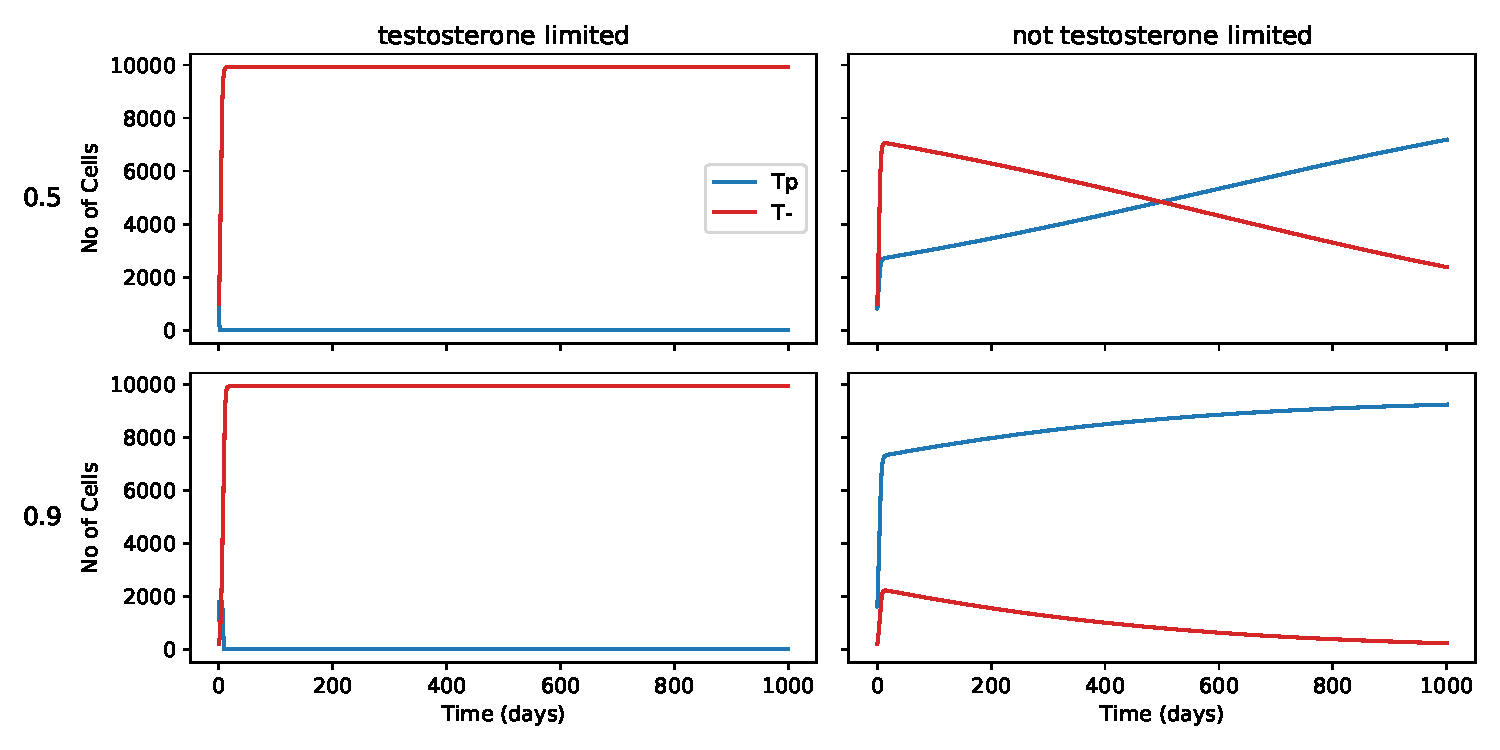
\includegraphics[width=\textwidth]{Tpro-Tneg_testlims}
  \caption[Pairwise $T^p - T^-$ time-series, testosterone limitation]{Pairwise $T^p - T^-$ time-series, when $T^p$ is testosterone limited and not testosterone limited (columns) and at different initial proportions of $T^p$ (rows). $T^p$ is testosterone limited at $ul_{test,T^p}=0.5$ and not testosterone limited at $ul_{test,T^p}=0.1$.}
  \label{fig_Tpro-Tneg_testlims}
\end{figure}

\begin{figure}[h!]
  \centering
  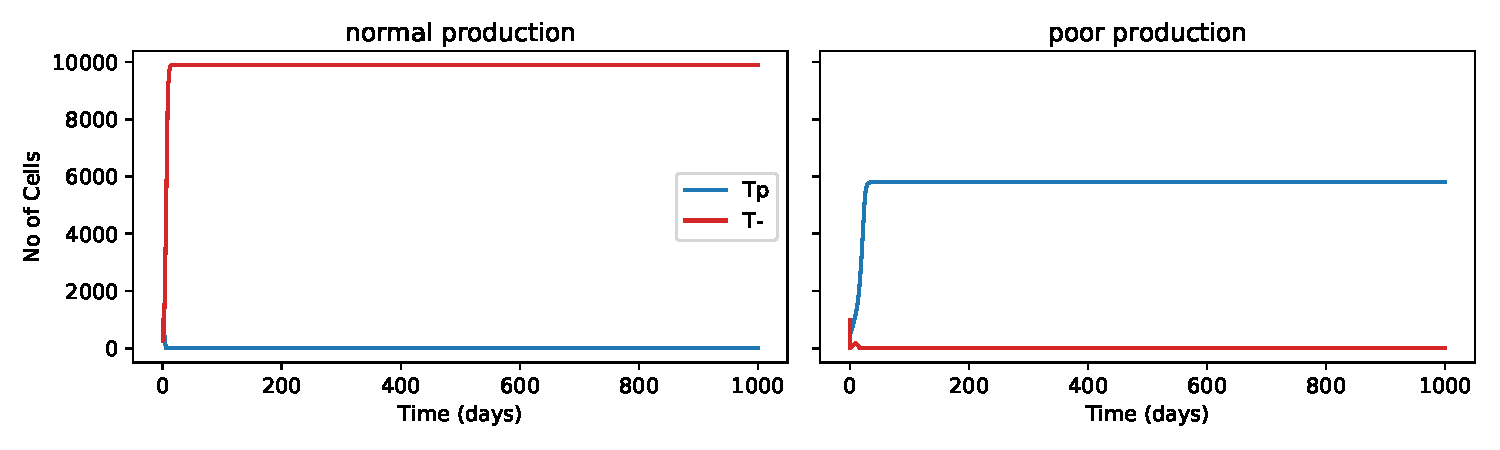
\includegraphics[width=\textwidth]{Tpro-Tneg_o2lims}
  \caption[Pairwise $T^p - T^-$ time-series, oxygen limitation]{Pairwise $T^p - T^-$ time-series, when $T^-$ is oxygen limited and at different oxygen production (column). $T^-$ is oxygen limited at $ll_{O_2,T^-}=0.6$ and $T^p$ is testosterone limited at $ul_{test,T^p}=0.5$. The normal and poor production of oxygen are 0.11 and 0.0675 min$^{-1}$ respectively}
  \label{fig_Tpro-Tneg_o2lims}
\end{figure}

Taken together, these provide the first proof-of-concept that competitive outcomes can be controlled through the interaction of cell types with the resources in the environment.

\newpage

Building on these initial observations, a brute force parameter space exploration was done over a large combination of parameters. The entire dataset is large and a few generalised observations collated from these data have been listed below.
\begin{enumerate}
  \item $T^-$ drives $T^p$ to extinction when $ll_{O_2,T^p} \geq 0.6$, regardless of the other parameters; in other words, $T^p$ should not be limited by oxygen if it is to compete with $T^-$.
  \item $T^-$ drives $T^p$ to extinction when $ll_{test,T^p} \geq 0.2$, regardless of the other parameters; in other words, $T^p$ needs to be able to grow even on the smallest amount of testosterone to compete with $T^-$.
  \item $T^-$ drives $T^p$ to extinction when $ul_{test,T^p} \geq 0.3$ and $ll_{O_2,T^-} \leq 0.4$ but not when $ll_{O_2,T^-} \geq 0.6$; in other words, $T^p$ shouldn’t be testosterone limited when $T^-$ is not oxygen limited to be to compete with $T^-$. The $ul_{test,T^p}$ required for $T^p$ to not go extinct also increases with increased $ll_{O_2,T^-}$, that is, $T^p$ can afford to be more testosterone limited as $T^-$ becomes more oxygen limited.
\end{enumerate}

These observations allow us to then define levels of resource limitation for each cell type, which represent the competitive strategy employed by that cell type. We fix three levels each of $T^p\ test$ limitation: no, moderate and severe corresponding to $ul_{test,T^p}=0.1, 0.3, 1$ respectively and three levels each of $T^-\ O_2$ limitation: low, high and severe corresponding to $ll_{O_2,T^-}=0, 0.6, 0.8$ respectively. As found earlier, $T^p$ goes extinct at any level of oxygen limitation and therefore offers no scope for exploration along this axis. We also explore two levels of $O_2$ production: normal and poor, corresponding to $p_{O_2}=0.11, 0.0675$ min$^{-1}$ respectively. Pairwise competitive runs were done over all combinations of these (as shown in \autoref{tab_Tpro-Tneg_cases}) with varying initial cell seeding.

\begin{table}
  \centering
  \begin{tabular}{|l|l|l|}
    \hline
    \textbf{$\boldsymbol{O_2}$ production} & \textbf{$\boldsymbol{T^-\ O_2}$ limitation} & \textbf{$\boldsymbol{T^p\ test}$ limitation}\\ \hline
    normal & low & no \\ \hline
    normal & low & moderate \\ \hline
    normal & low & severe \\ \hline
    normal & high & no \\ \hline
    normal & high & moderate \\ \hline
    normal & high & severe \\ \hline
    normal & severe & no \\ \hline
    normal & severe & moderate \\ \hline
    normal & severe & severe \\ \hline
    poor & low & no \\ \hline
    poor & low & moderate \\ \hline
    poor & low & severe \\ \hline
    poor & high & no \\ \hline
    poor & high & moderate \\ \hline
    poor & high & severe \\ \hline
    poor & severe & no \\ \hline
    poor & severe & moderate \\ \hline
    poor & severe & severe \\ \hline
  \end{tabular}
  \caption{Table of cases for $T^p$ - $T^-$ pairwise}
  \label{tab_Tpro-Tneg_cases}
\end{table}

\newpage

The following were observed from the cases as visualised in \autoref{fig_Tpro-Tneg_cases}:
\begin{enumerate}
  \item Coexistence is observed only when there is no or moderate limitation of testosterone for $T^p$ and low limitation of oxygen for $T^-$. For low $T^p$ initial seeding, $T^-$ dominates over $T^p$ and causes it to go extinct, but as $T^p$ initial seeding increases the favour shifts towards $T^p$.
  \item $T^-$ causes $T^p$ to go extinct for all initial seedings when $T^p$ is severely testosterone limited. Even with a high initial seeding advantage, $T^-$ grows, overtakes $T^p$ and eventually causes $T^p$ to go extinct. $T^-$ also goes extinct in this case if it is limited by oxygen under poor oxygen production. Despite this, $T^p$ is weighed down by both the testosterone limitation and density-dependent competition of the remaining $T^-$ cells and goes extinct as a result.
  \item The outcome switches from $T^p$ going extinct to $T^-$ going extinct for higher $T^p$ initial seeding when $T^-$ is highly limited by oxygen under either poor or normal oxygen production and when $T^-$ is severely limited by oxygen under normal oxygen production. Similar to the cases with coexistence, for low $T^p$ initial seeding, $T^-$ dominates over $T^p$ and causes it to go extinct, but as $T^p$ initial seeding increases the favour shifts towards $T^p$. However, in this case the oxygen levels don’t go above the levels required for $T^-$ to grow before it goes extinct and only $T^p$ remains.
  \item $T^-$ goes extinct for all initial seedings when it is severely oxygen limited under poor oxygen production. The oxygen limitation on $T^-$ is too high and the oxygen levels never reach the levels required for a non-zero growth for $T^-$.
  \item Additionally, total population size has a weaker effect than initial proportion for the dynamics and outcomes for each particular case.
\end{enumerate}

These observations expand and broaden the scope of the earlier finding that cell-intrinsic doubling times have a relatively marginal effect on competitive outcome; with the data in \autoref{fig_Tpro-Tneg_cases}, it is possible to pinpoint which resource conditions favour each cell type based on their relative limitation strengths for that resource.

\begin{figure}[h!]
  \centering
  \begin{subfigure}[b]{\textwidth}
    \centering
    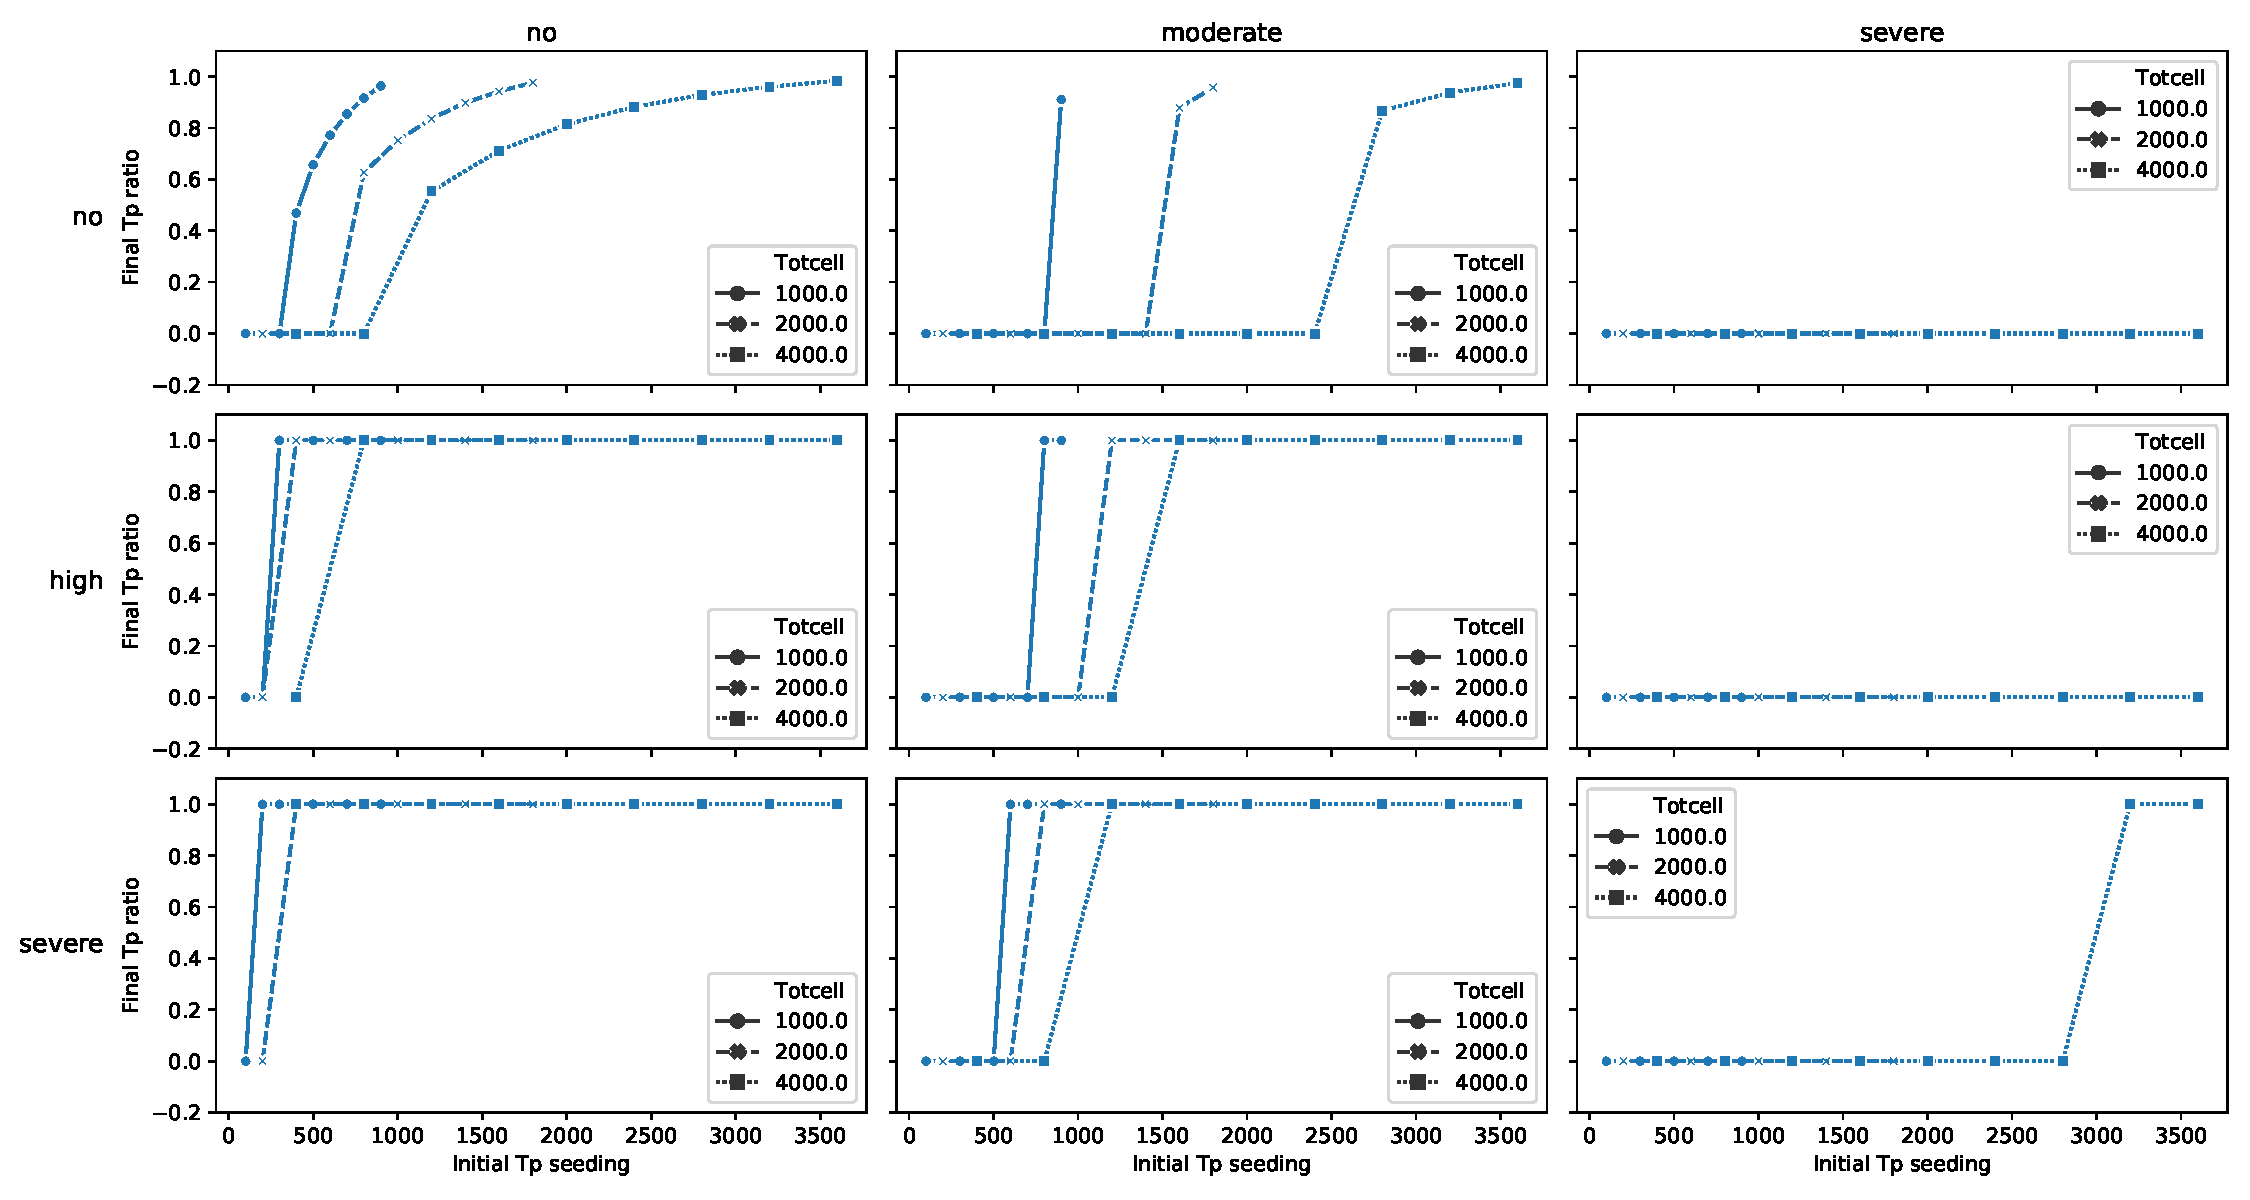
\includegraphics[width=\textwidth]{Tpro-Tneg_cases_normal}
    \caption{normal production}
    \label{fig_Tpro-Tneg_cases_normal}
  \end{subfigure}
  \begin{subfigure}[b]{\textwidth}
    \centering
    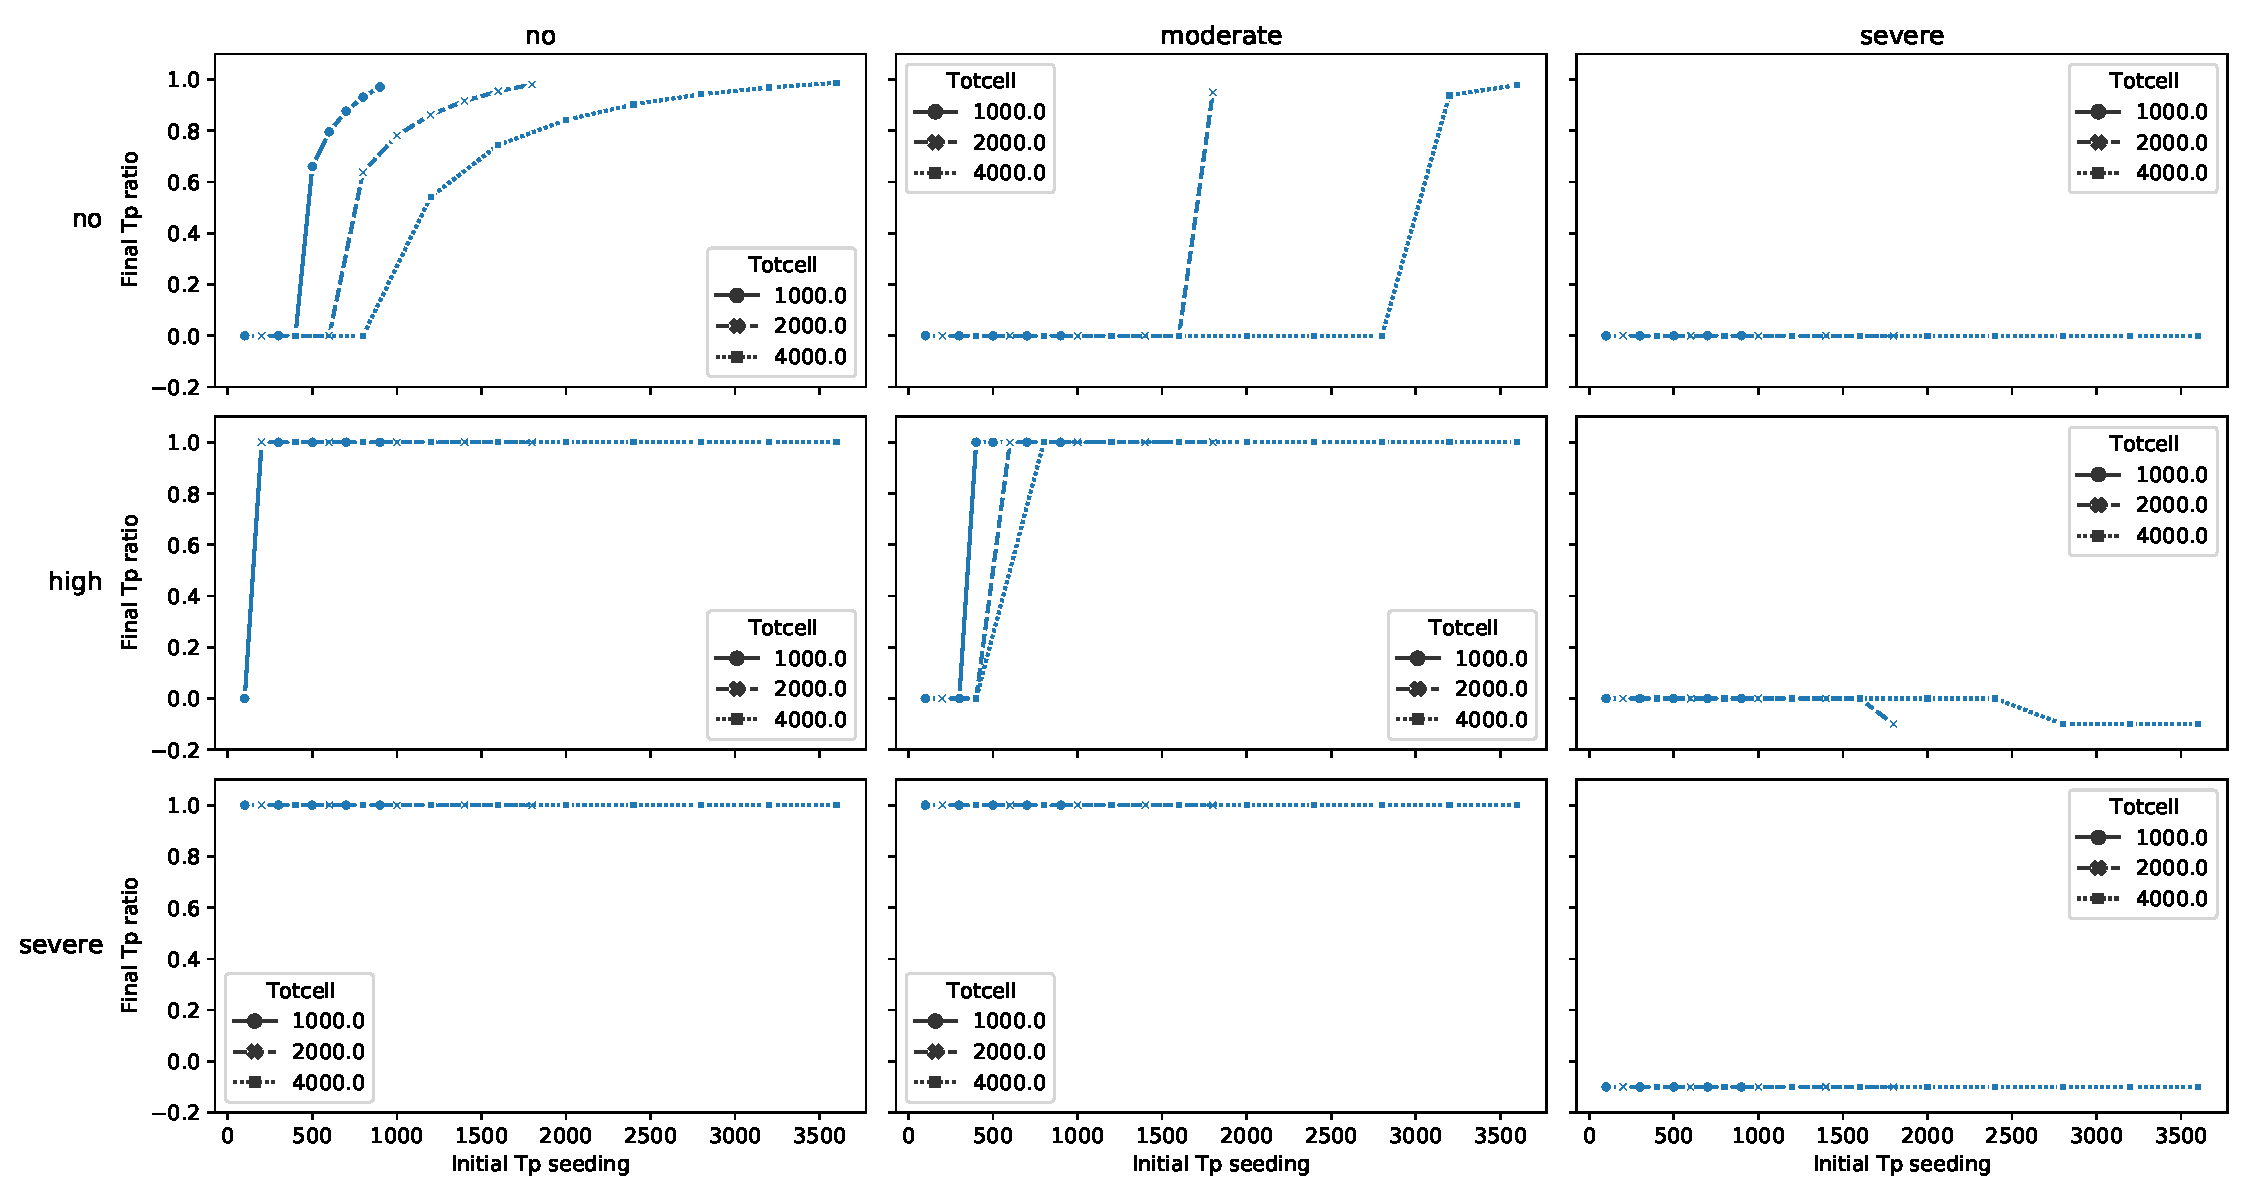
\includegraphics[width=\textwidth]{Tpro-Tneg_cases_poor}
    \caption{poor production}
    \label{fig_Tpro-Tneg_cases_poor}
  \end{subfigure}
  \caption[Final $T^p$ ratio of pairwise $T^p - T^-$ runs under different cases]{Final $T^p$ ratio of pairwise $T^p - T^-$ runs under different cases. Subfigures: $O_2$ Production, Rows: $T^-\ O_2$ limitation, Columns: $T^p\ test$ limitation. Note: Ratio = -0.1 is used when both cell types go extinct.}
  \label{fig_Tpro-Tneg_cases}
\end{figure}

\clearpage

\section{$\boldsymbol{T^+}$ - $\boldsymbol{T^p}$}
The initial runs for this pair involved changing both the upper and lower limits of the resource response function together as a way of sampling resource limitation conditions coarsely before a more detailed exploration. The following observations were made based on these results, represented in \autoref{fig_Tpos-Tpro_o2lims} and \autoref{fig_Tpos-Tpro_testlims}:
\begin{enumerate}
    \item Both $T^+$ and $T^p$ are limited by both oxygen and testosterone, and compete for both resources. As with the other pair, strength of limitation for any particular resource can be modulated through the corresponding upper and lower thresholds.
    \item When $T^p$ is limited by testosterone more than $T^+$ ($ul_{test,T^p} > ul_{test,T^+}$), $T^+$ can consume and grow on the limited testosterone present, and this is enough for the density-dependent competition to drive $T^p$ to extinction. Without $T^p$ to provide testosterone, $T^+$ subsequently goes extinct.
    \item When $T^p$ is weakly limited by testosterone relative to $T^+$ ($ul_{test,T^p} \leq ul_{test,T^+}$), both cells coexist. Due to weaker testosterone limitation, $T^p$ can grow faster initially and secrete enough testosterone for $T^+$ without being negatively affected by $T^+$. This is visualised in \autoref{fig_Tpos-Tpro_testlims}.
    \item When both are severely testosterone limited but not oxygen limited, $T^p$ causes $T^+$ to go extinct. However, in a special scenario when both are oxygen limited with $T^+$ being more limited, coexistence is observed. A balance of sort is achieved here, where, in the initial period of low oxygen, $T^p$ can grow more than $T^+$ and secrete enough testosterone to sustain both population but doesn’t grow as much as to drive $T^+$ to extinction. This is visualised in \autoref{fig_Tpos-Tpro_o2lims}.
  \end{enumerate}

\begin{figure}[h!]
  \centering
  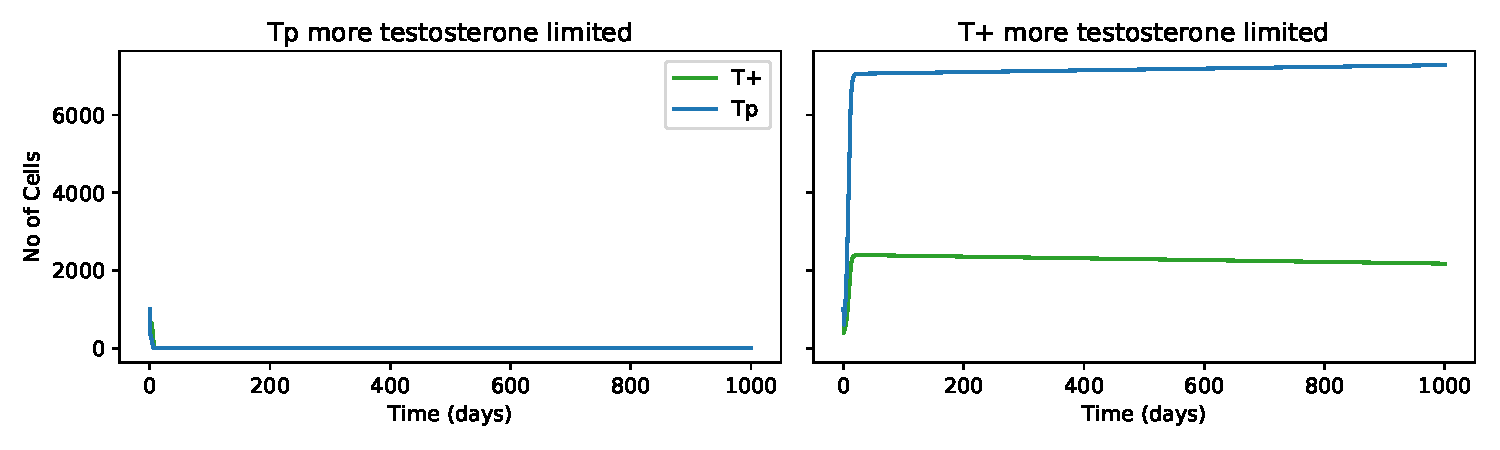
\includegraphics[width=\textwidth]{Tpos-Tpro_testlims}
  \caption[Pairwise $T^+ - T^p$ time-series, testosterone limitation]{Pairwise $T^+ - T^p$ time-series, when $T^p$ is more testosterone limited than $T^+$ and when $T^+$ is more testosterone limited than $T^p$. $T^p$ is more limited testosterone limited at $ul_{test,T^+}=0.3,ul_{test,T^p}=0.5$ and $T^+$ is limited more at $ul_{test,T^+}=0.5,ul_{test,T^p}=0.3$.}
  \label{fig_Tpos-Tpro_testlims}
\end{figure}

\begin{figure}[h!]
  \centering
  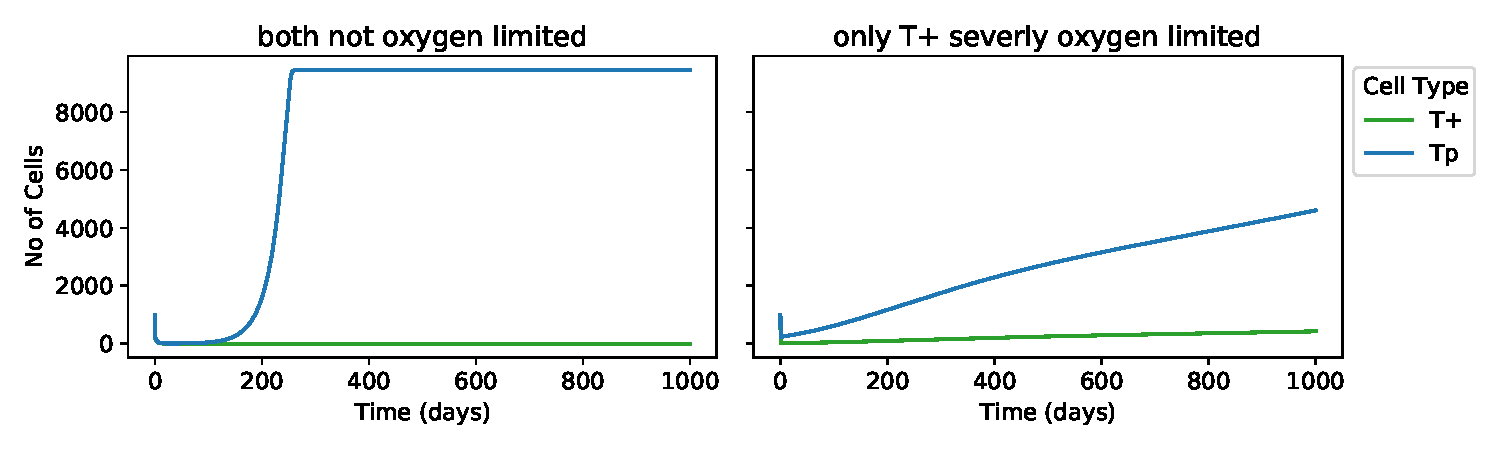
\includegraphics[width=\textwidth]{Tpos-Tpro_o2lims}
  \caption[Pairwise $T^+ - T^p$ time-series, oxygen limitation]{Pairwise $T^+ - T^p$ time-series, when both cell types are testosterone limited and not oxygen limited at $ll_{O_2,T^+}=0.0, ll_{O_2,T^p}=0.0$ and $T^+$ is oxygen limited and $T^p$ moderately at $ll_{O_2,T^+}=0.6, ll_{O_2,T^p}=0.4$.}
  \label{fig_Tpos-Tpro_o2lims}
\end{figure}

As with $T^p-T^-$, cell type competitive strategies were encoded in terms of levels of resource limitation for each cell type. Three levels each of $T^p\ test$ and $T^+\ test$ limitation: no, moderate and severe corresponding to $ul_{test,T^i}=0.1, 0.3, 1$ respectively, Three levels each of $T^p\ O_2$ and $T^+\ O_2$ limitation: low, moderate and severe corresponding to $ll_{O_2,T^i}=0, 0.4, 0.8$ respectively were considered and pairwise competitive runs were done over some combinations of these (as shown in \autoref{tab_Tpos-Tpro_cases}) with varying initial cell seeding.

Only two levels of limitations were considered for each resource when combinations of both $O_2$ or $test$ limitations were done to reduce the number of combinations for better interpretability. Similarly, different levels of $O_2$ or $test$ production is not considered in these cases for the same reason. Production terms will ultimately affect resource availability, and adjusting the response function of the cell should be qualitatively equivalent to reducing actual resource concentrations.

\begin{table}
  \centering
  \begin{tabular}{|l|l|l|l|}
    \hline
    \textbf{$\boldsymbol{T^+\ O_2}$ limitation} & \textbf{$\boldsymbol{T^p\ O_2}$ limitation} & \textbf{$\boldsymbol{T^+\ test}$ limitation} & \textbf{$\boldsymbol{T^p\ test}$ limitation}  \\ \hline
    low & low & no & no \\ \hline
    low & low & no & moderate \\ \hline
    low & low & no & severe \\ \hline
    low & low & moderate & no \\ \hline
    low & low & moderate & moderate \\ \hline
    low & low & moderate & severe \\ \hline
    low & low & severe & no \\ \hline
    low & low & severe & moderate \\ \hline
    low & low & severe & severe \\ \hline
    low & moderate & no & no \\ \hline
    low & moderate & no & moderate \\ \hline
    low & moderate & moderate & no \\ \hline
    low & moderate & moderate & moderate \\ \hline
    low & severe & no & no \\ \hline
    moderate & low & no & no \\ \hline
    moderate & low & no & moderate \\ \hline
    moderate & low & moderate & no \\ \hline
    moderate & low & moderate & moderate \\ \hline
    moderate & moderate & no & no \\ \hline
    moderate & moderate & no & moderate \\ \hline
    moderate & moderate & moderate & no \\ \hline
    moderate & moderate & moderate & moderate \\ \hline
    moderate & severe & no & no \\ \hline
    severe & low & no & no \\ \hline
    severe & moderate & no & no \\ \hline
    severe & severe & no & no \\ \hline
  \end{tabular}
  \caption{Table of cases for $T^+$ - $T^p$ pairwise}
  \label{tab_Tpos-Tpro_cases}
\end{table}

\newpage

The following were observed from the different cases. For better visualisation, the figures are divided into testosterone limitations in \autoref{fig_Tpos-Tpro_cases_test}, oxygen limitations in \autoref{fig_Tpos-Tpro_cases_o2} and combinations of the limitations in \autoref{fig_Tpos-Tpro_cases_combi}.
\begin{enumerate}
  \item Severe limitation of either oxygen or testosterone for $T^+$ relative to $T^p$ causes it to go extinct. In a special case, when $T^p$ numbers are high enough to produce an excess of testosterone, a small fraction of $T^+$ survives regardless of the strength of $T^+$ test limitation. Conversely, when neither resource is limiting, coexistence occurs at all seeding densities and proportions of $T^p$, which suggests that competitive exclusion of either cell type is strongly dependent on environmental conditions and resource limitation. When $T^+$ is moderately oxygen limited relative to $T^p$, $T^+$ can coexist at low initial density of $T^p$ but goes extinct at higher initial densities.
  \item $T^p$ is driven to extinction in every case where $T^p$ limitation of either oxygen or testosterone is more severe relative to $T^+$ limitation of the same resource. Extinction of $T^p$ then leads to extinction of $T^+$ trivially. Such is the case for the most part with moderate limitation of testosterone for $T^p$ relative to $T^+$. However, this $T^p$ extinction is seen to be rescued for higher initial density of $T^p$ relative to $T^+$ as this allows the former to overcome competition, leading to coexistence.
  \item In very broad terms, coexistence is more common when the strength of limitation of either resource is the same for both cell types-these are the main diagonals in \autoref{fig_Tpos-Tpro_cases_test} and \autoref{fig_Tpos-Tpro_cases_o2}. Generally, increasing the relative proportion of $T^p$ gives it a competitive edge presumably by increasing net availability of testosterone in the system. However, under high testosterone limitation for both cell types, a larger $T^p$ proportion is marginally detrimental to $T^p$ success possibly due to density-dependent intraspecific competition.
  \item With moderate limitation of oxygen for $T^p$ relative to $T^+$, $T^+$ still requires testosterone from $T^p$ for survival which could weaken the growth inhibition of $T^p$, despite the lower oxygen limitation of $T^+$ compared to $T^p$. Interestingly, this is also the case with coexistence at lower final $T^p$ proportions than any other case. Coexistence here is therefore driven by the dependence on $T^p$ by $T^+$ for testosterone, which overrides any advantage from a better oxygen use strategy.
  \item Coexistence is also observed when $T^+$ is moderately testosterone limited relative to $T^p$. However, in this case, a lower initial proportion of $T^p$ favours $T^p$ and leads to a dip in the plot. At a low initial proportion of $T^p$, $T^+$ being limited by testosterone dies out until sufficient testosterone is established and this might give an advantage for $T^p$ to establish a larger population before $T^+$ has the capacity to compete.
  \item The behaviour of the system is very similar if the resource limitation is symmetric across the two cell types. This can be seen from the first and last columns or from the first and last rows of \autoref{fig_Tpos-Tpro_cases_combi}. Although, with the higher testosterone limitations of $T^p$, a higher $T^p$ initial seeding is required to have $T^p$ overcome suppression by $T^+$. Additionally, when $T^p$ is moderately limited by oxygen relative to $T^+$, the higher testosterone limitation of $T^+$ leads to higher $T^p$ required for the testosterone.
  \item When both testosterone and oxygen are moderately limiting for a cell type relative to the other, the combined overall limitation is severe and that particular cell type is driven to extinction similar to when only one resource was severely limiting.
  \item When $T^p$ is moderately limited by oxygen relative to $T^+$ and $T^+$ moderately limited by testosterone relative to $T^p$, a balance is achieved. $T^+$ can outcompete $T^p$ due to the excess oxygen but soon is limited by testosterone and has to allow a sizeable population of $T^p$ to grow to maintain the required testosterone levels. However, with the inverse case where $T^p$ is testosterone limited and $T^+$ is oxygen limited, the outcomes are unstable and it switches from $T^p$ driven to extinction at low initial proportion to $T^+$ going extinct for higher initial proportion.
  \item Additionally, total population size has a weaker effect than initial proportion for the dynamics and outcomes for each particular case.
\end{enumerate}

\begin{figure}[h!]
  \centering
  \begin{subfigure}[b]{\textwidth}
    \centering
    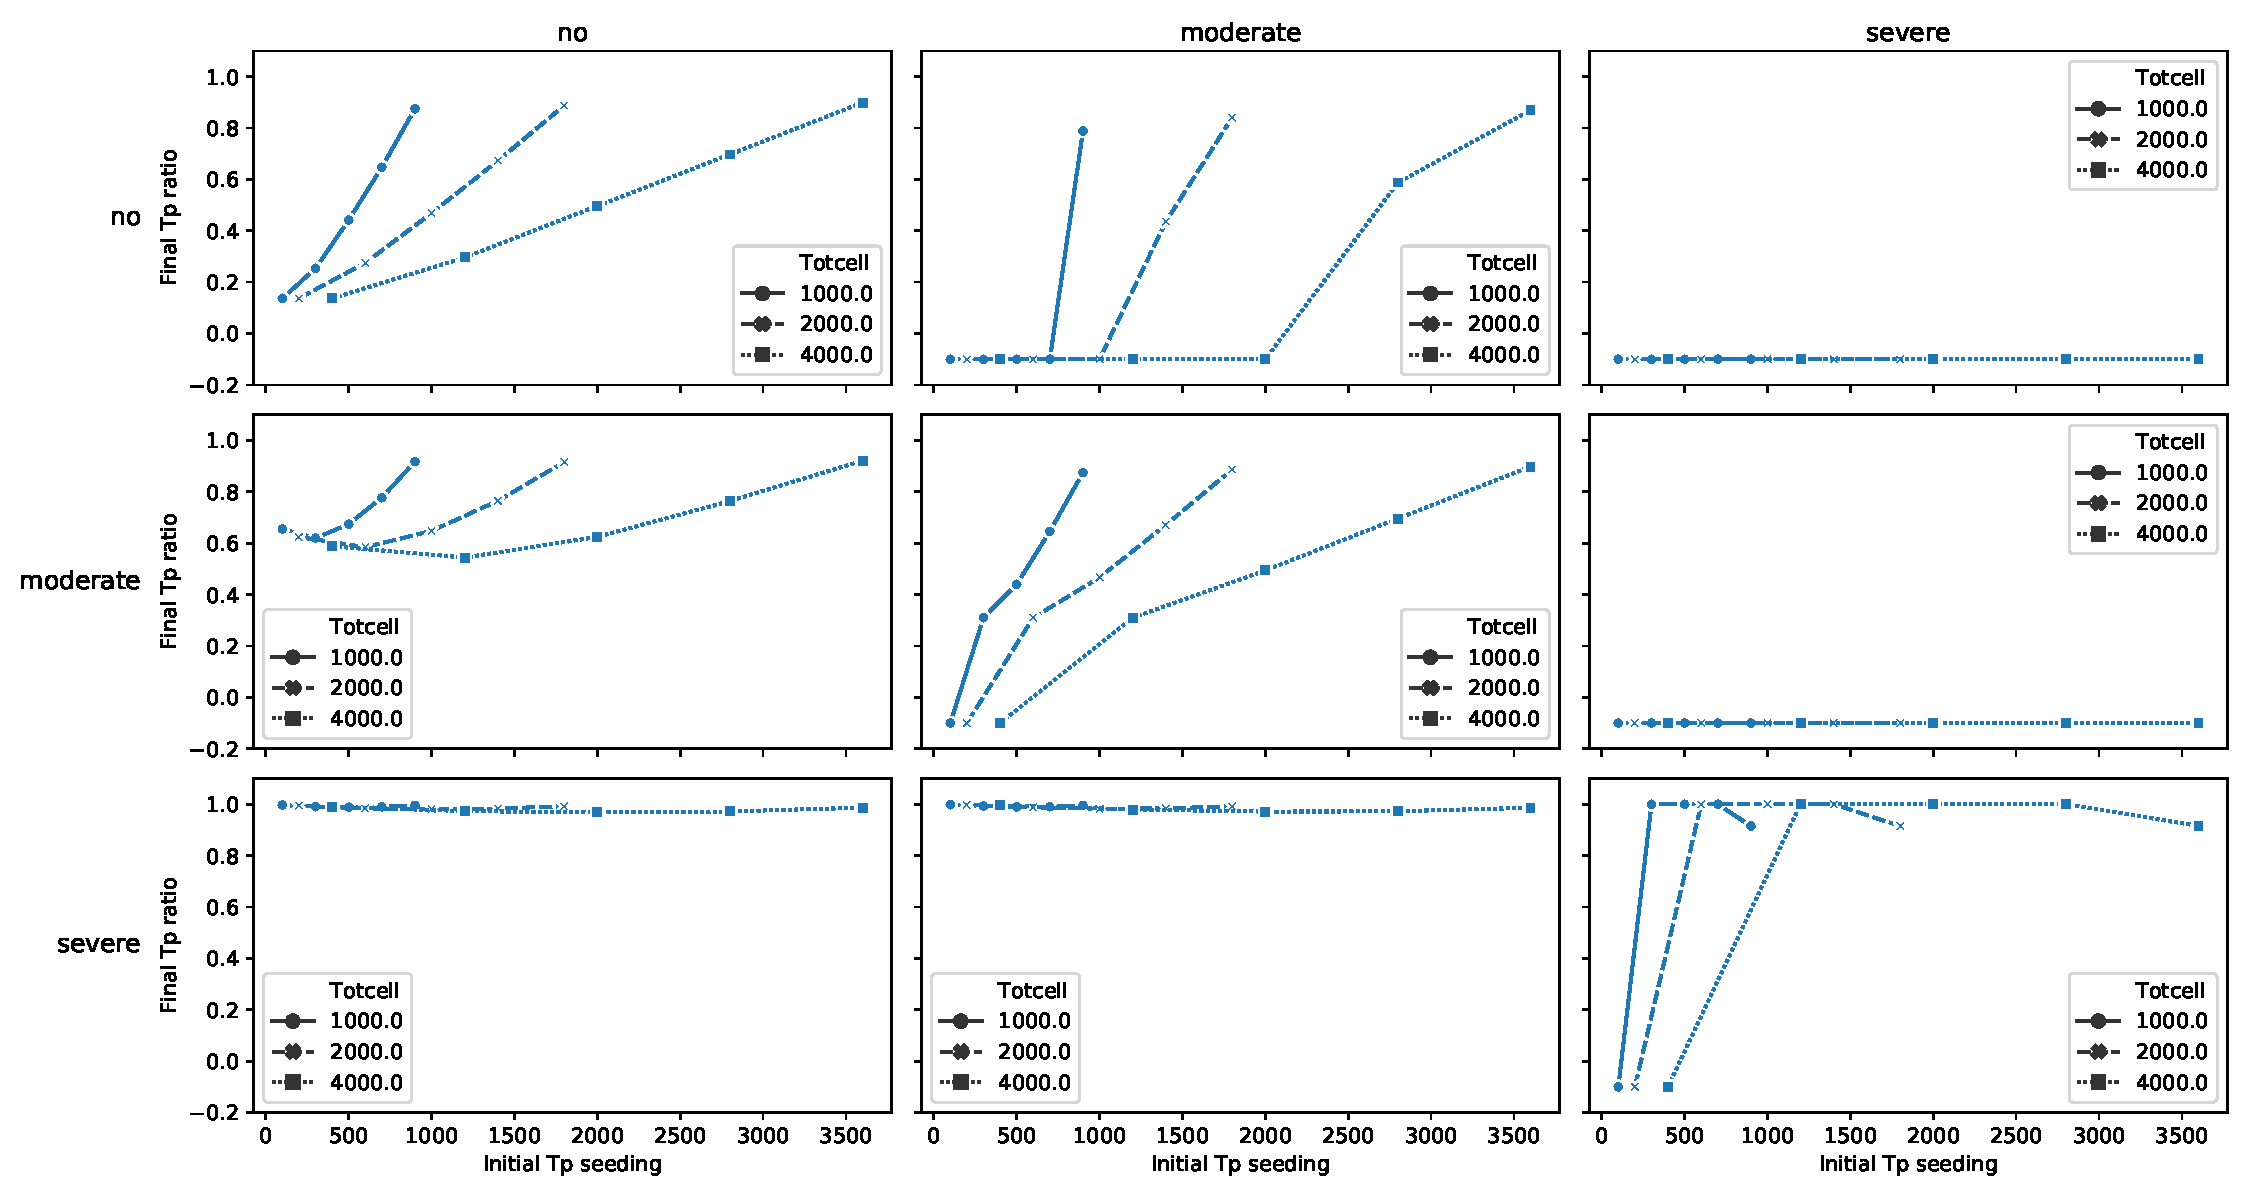
\includegraphics[width=\textwidth]{Tpos-Tpro_cases_test}
    \caption{$test$ limitations. Columns: $T^p\ test$ limitation, Rows: $T^+\ test$ limitation.}
    \label{fig_Tpos-Tpro_cases_test}
  \end{subfigure}
  \begin{subfigure}[b]{\textwidth}
    \centering
    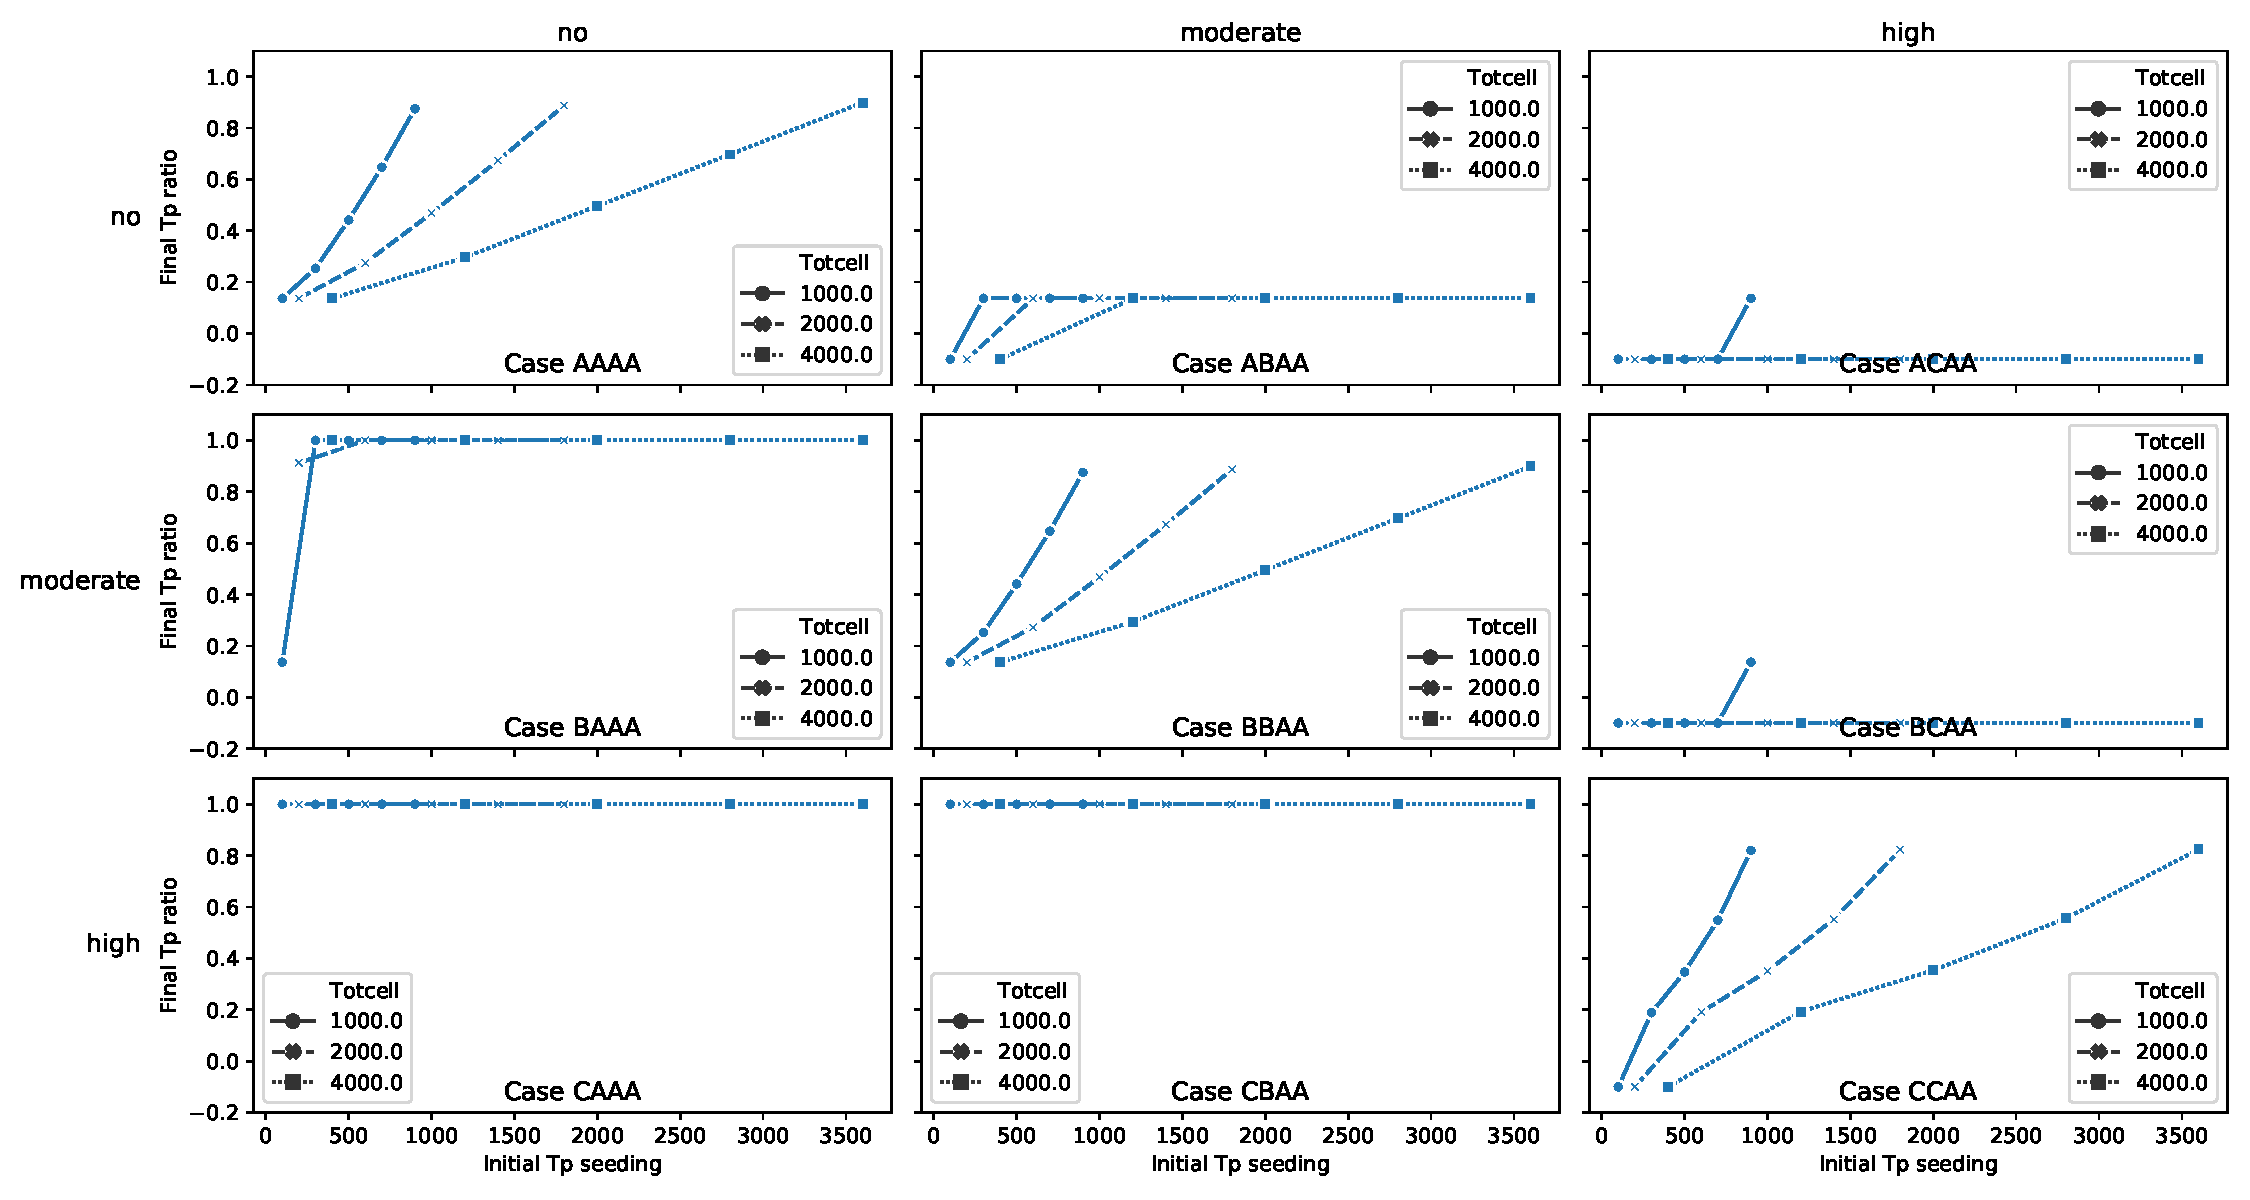
\includegraphics[width=\textwidth]{Tpos-Tpro_cases_o2}
    \caption{$O_2$ limitations. Columns: $T^p\ O_2$ limitation, Rows: $T^+\ O_2$ limitation.}
    \label{fig_Tpos-Tpro_cases_o2}
  \end{subfigure}
  \caption[]{(Continued on next page)}
\end{figure}
\begin{figure}[h!]\ContinuedFloat
  \centering
  \begin{subfigure}[b]{\textwidth}
    \centering
    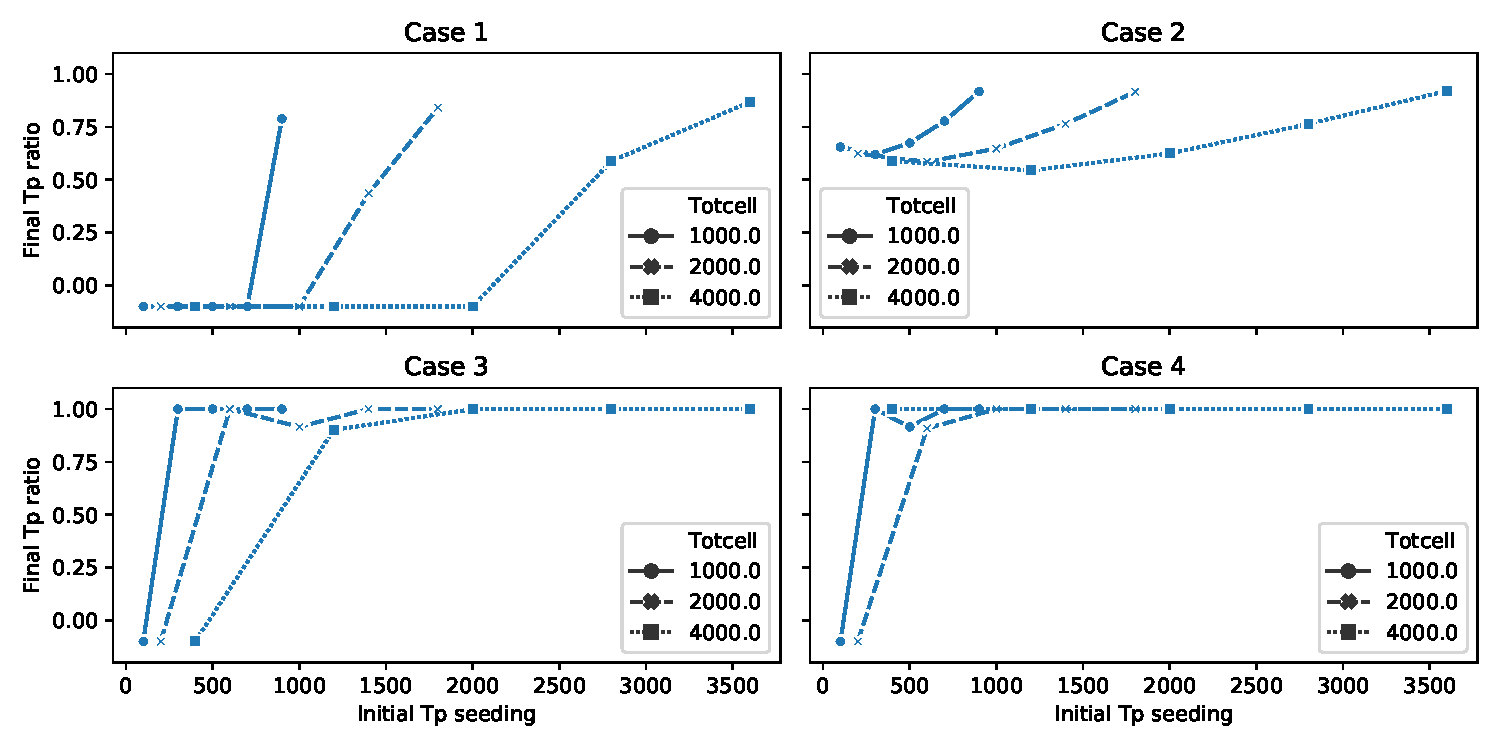
\includegraphics[width=\textwidth]{Tpos-Tpro_cases}
    \caption{Combination  of $test$ and $O_2$ limitations. Columns: $T^+,T^p\ test$ limitations, Rows: Columns: $T^+,T^p\ O_2$ limitations.}
    \label{fig_Tpos-Tpro_cases_combi}
  \end{subfigure}
  \caption[Final $T^p$ ratio of pairwise $T^+ - T^p$ runs under different cases]{Final $T^p$ ratio of pairwise $T^+ - T^p$ runs under different cases. Note: Ratio = -0.1 is used when both cell types go extinct.}
  \label{fig_Tpos-Tpro_cases}
\end{figure}

\chapter{All cell types-interactions and competition outcomes}
With all three cell types, the number of combinations and permutations increase combinatorially which restricts the tractability of giving different strategies to each cell type as has been done with the pairwise simulations. We are therefore starting with a simpler case of the same strategy for all the three cell types. The strategies are still defined in terms of levels of resource limitations, with the distinction that now, the level of each strategy is the same for all the three cell types. The values of lower and upper limits corresponding to each level are given in \autoref{tab_all3_limits}.

\begin{table}
\centering
  \begin{tabular}{|l|l|l|l|}
    \hline
    \textbf{Resource} & \textbf{Limitation} & \textbf{$\boldsymbol{ll_{res,i}}$} & \textbf{$\boldsymbol{ul_{res,i}}$} \\ \hline
    \multirow{3}{*}{Oxygen} & no & 0.0 & 1.1 \\ \cline{2-4}
    & low & 0.0 & 1.0 \\ \cline{2-4}
    & moderate & 0.4 & 0.1 \\ \hline
    \multirow{3}{*}{Testosterone} & no & 0 & 0.1 \\ \cline{2-4}
    & moderate & 0 & 0.3 \\ \hline
  \end{tabular}
  \caption[Table of resource limitations for all cell types]{Table of limits corresponding to limitations for different resources of all three cell-types}
  \label{tab_all3_limits}
\end{table}

\newpage

Competitive runs were done over all the six combinations of limitations for two different ratios of seeding and three initial total seedings. The following were observed from the different cases as visualised in \autoref{fig_all3}. The time-series of the same is given in \autoref{fig_all3-time-series}.
\begin{enumerate}
  \item Moderate limitation of testosterone leads to  stronger interspecific competition relative to intraspecific competition as $T^p$ and $T^+$ numbers cannot increase enough to produce self-inhibition. In these cases, inhibition by $T^-$ is much stronger and they are driven to extinction, as opposed to when $T^p$ and $T^+$ coexisted when seeded without $T^-$. However, consistent with the $T^p - T^+$ results, coexistence can be recovered between all three cell types when $T^p$ is seeded at a much higher proportion than the other two, presumably because of higher net available testosterone in the system. Therefore, when testosterone is a strongly limiting resource, it also leads to strong positive dependence on $T^p$ density for coexistence.
  \item No limitation of testosterone leads to weaker interspecific competition relative to intraspecific competition, but only above a threshold proportion of $T^p$ that is required to produce a minimum amount of testosterone for survival. Again, we see that self-production of testosterone by $T^p$ leads to progressively lower limitation of the hormone across runs with increasing number of $T^p$ cells, as well as within a given run with increasing time. Additionally, in the moderate testosterone limitation cases, it can be seen that lower oxygen limitation reinforces this positive feedback on $T^p$ further, leading to coexistence that is further biased towards the $T^p - T^+$ pair.
  \item Testosterone then acts as a private resource and the primary limitation between $T^p$ and $T^+$ that serves to produce positive feedback above some minimum test concentration, thus leading to coexistence between all three cell types even though $T^-$ has a significantly shorter doubling time.
\end{enumerate}
Taken together, the resource limitation space can be divided into three broad zones of cell type coexistence in the system. At high limitations of testosterone, the growth of $T^p$ is so strongly inhibited that coexistence is rare, independent of the availability of oxygen; indeed, the addition of oxygen limitation only drives $T^p$ down further and makes coexistence even more remote. At the other extreme of low limitation of testosterone, $T^p$ growth inhibition is relieved and the positive feedback from $T^p$-produced testosterone is strong enough that oxygen limitations become relatively less important for coexistence. This is abundantly clear from when $T^p$ is seeded at a much higher density than the other cell types [\autoref{fig_all3_8:1:1}]. Oxygen limitations are seen to impact coexistence only when testosterone availability is above some minimum threshold required for $T^p - T^+$ growth, but not so high as to saturate all growth. In this range of resource availability, within the limits of the parameter values tested here, continuous responses to change in resource concentration are observed, and the outcomes of competition are pushed either towards coexistence or extinction of $T^p$ and $T^+$ by the oxygen limitation. Therefore, across these three zones, limitations of oxygen seem to have a subordinate impact on competition and instead supplement the competition imposed by testosterone; where oxygen limitation does affect competitive outcomes, it does so in the same direction as testosterone limitation.

\begin{figure}[h!]
  \centering
  \begin{subfigure}[b]{\textwidth}
    \centering
    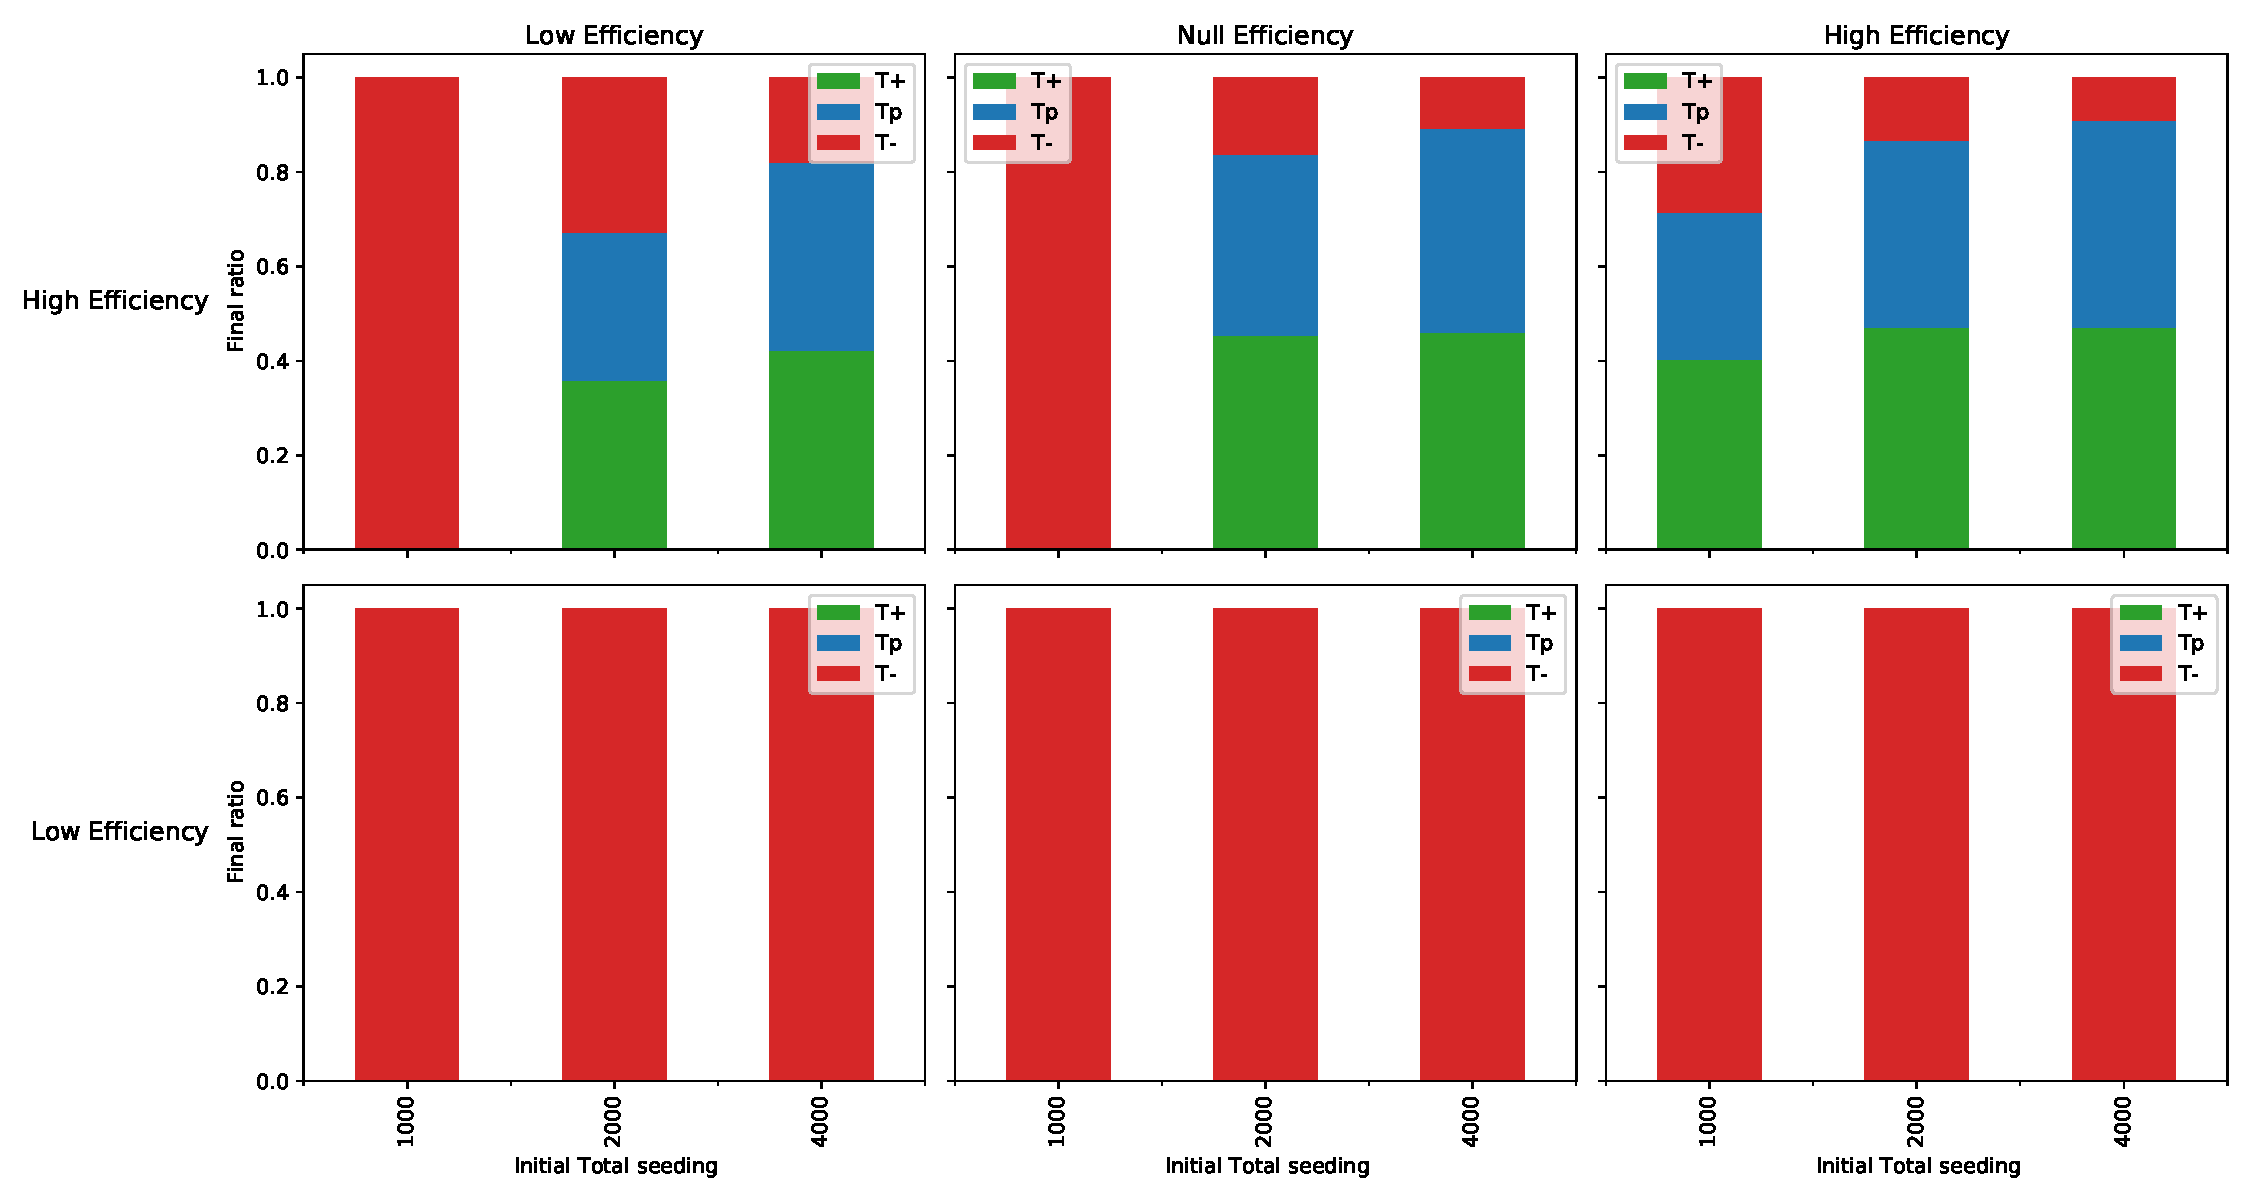
\includegraphics[width=\textwidth]{All3_efficiency_1:1:1}
    \caption{Equal Seeding - $T^p:T^+:T^-$ :: 1:1:1 }
    \label{fig_all3_1:1:1}
  \end{subfigure}
  \begin{subfigure}[b]{\textwidth}
    \centering
    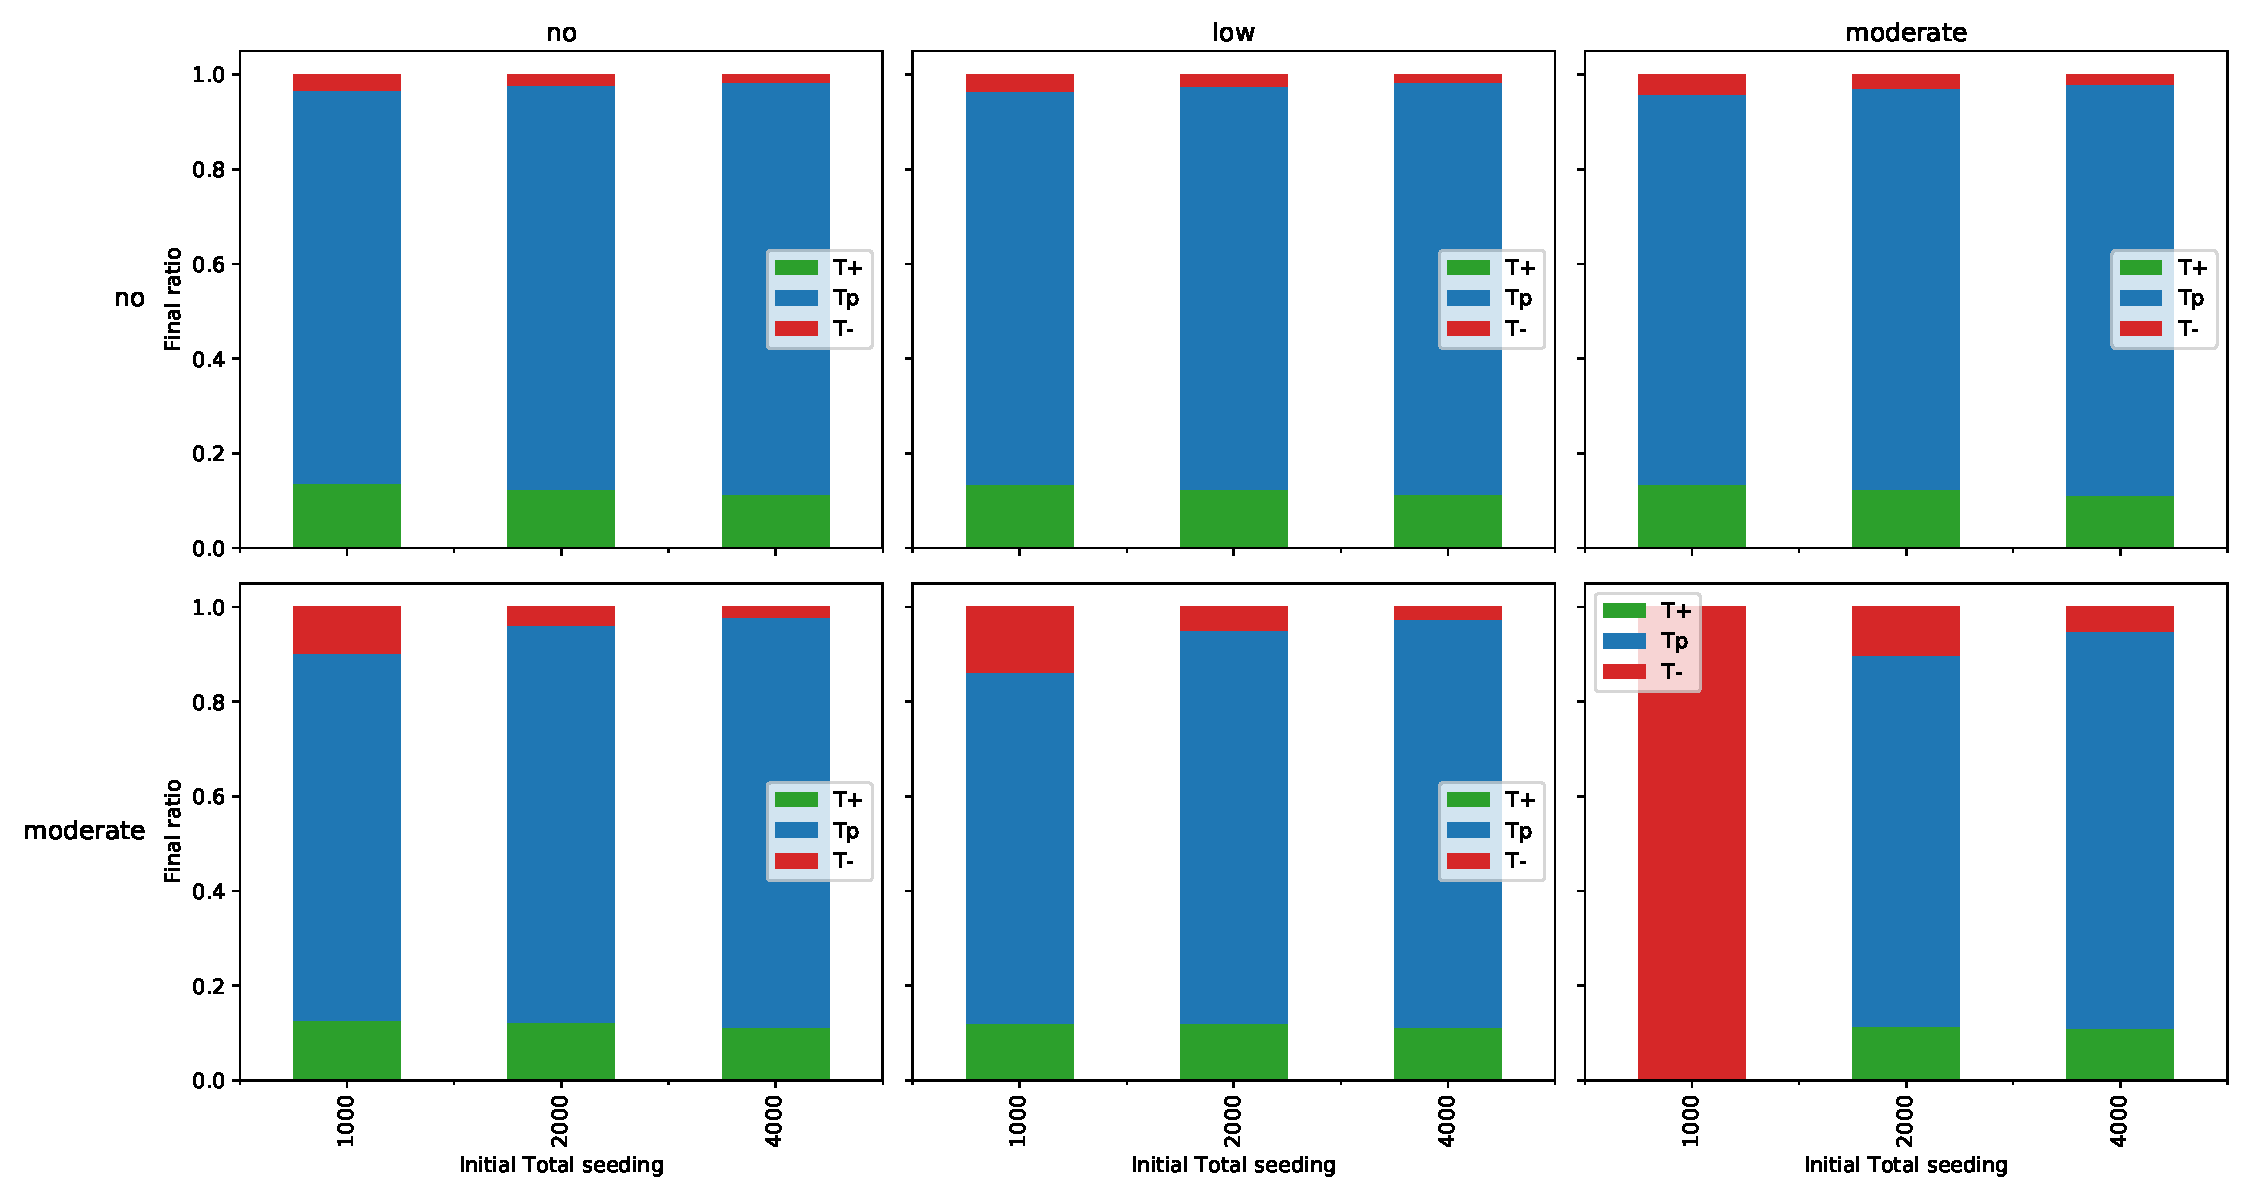
\includegraphics[width=\textwidth]{All3_efficiency_8:1:1}
    \caption{High $T^p$ seeding- $T^p:T^+:T^-$ :: 8:1:1}
    \label{fig_all3_8:1:1}
  \end{subfigure}
  \caption[Final ratio of all cell types under different limitations]{Final ratio of all cell types under different oxygen limitation (columns), testosterone limitation (rows) and initial seeding proportions (subfigures).}
  \label{fig_all3}
\end{figure}

\chapter{All cell types-therapy outcomes}
\section{Standard of care (SOC)}
Under standard-of-care, the drug is applied from the beginning of the simulation at the maximum tolerated dose for all the cases explored in the previous chapter. In our model, this is simulated as a permanently reduced rate of testosterone secretion by $T^p$.

We observe from \autoref{fig_therapy-SOC} that $T^+$ and $T^p$ go extinct in all the cases, regardless of the limitations of either resource, the seeding proportion or initial total seeding. This can be rationalised based on the results from the previous chapter, where testosterone limitation had a similarly drastic effect on coexistence, or lack thereof, between the three cell types. In this case, with therapy, the nearly immediate elimination of $T^+$ and $T^p$ due to insufficient levels of testosterone leads to competitive release of $T^-$, and the total population reaches its maximum effective carrying capacity. Given that abiraterone acts by suppressing testosterone secretion, an entire population of $T^-$ cells would be fully unresponsive to abiraterone treatment, and further treatment cannot lead to any reduction of cell number.

\begin{figure}[h!]
  \centering
  \begin{subfigure}[b]{\textwidth}
    \centering
    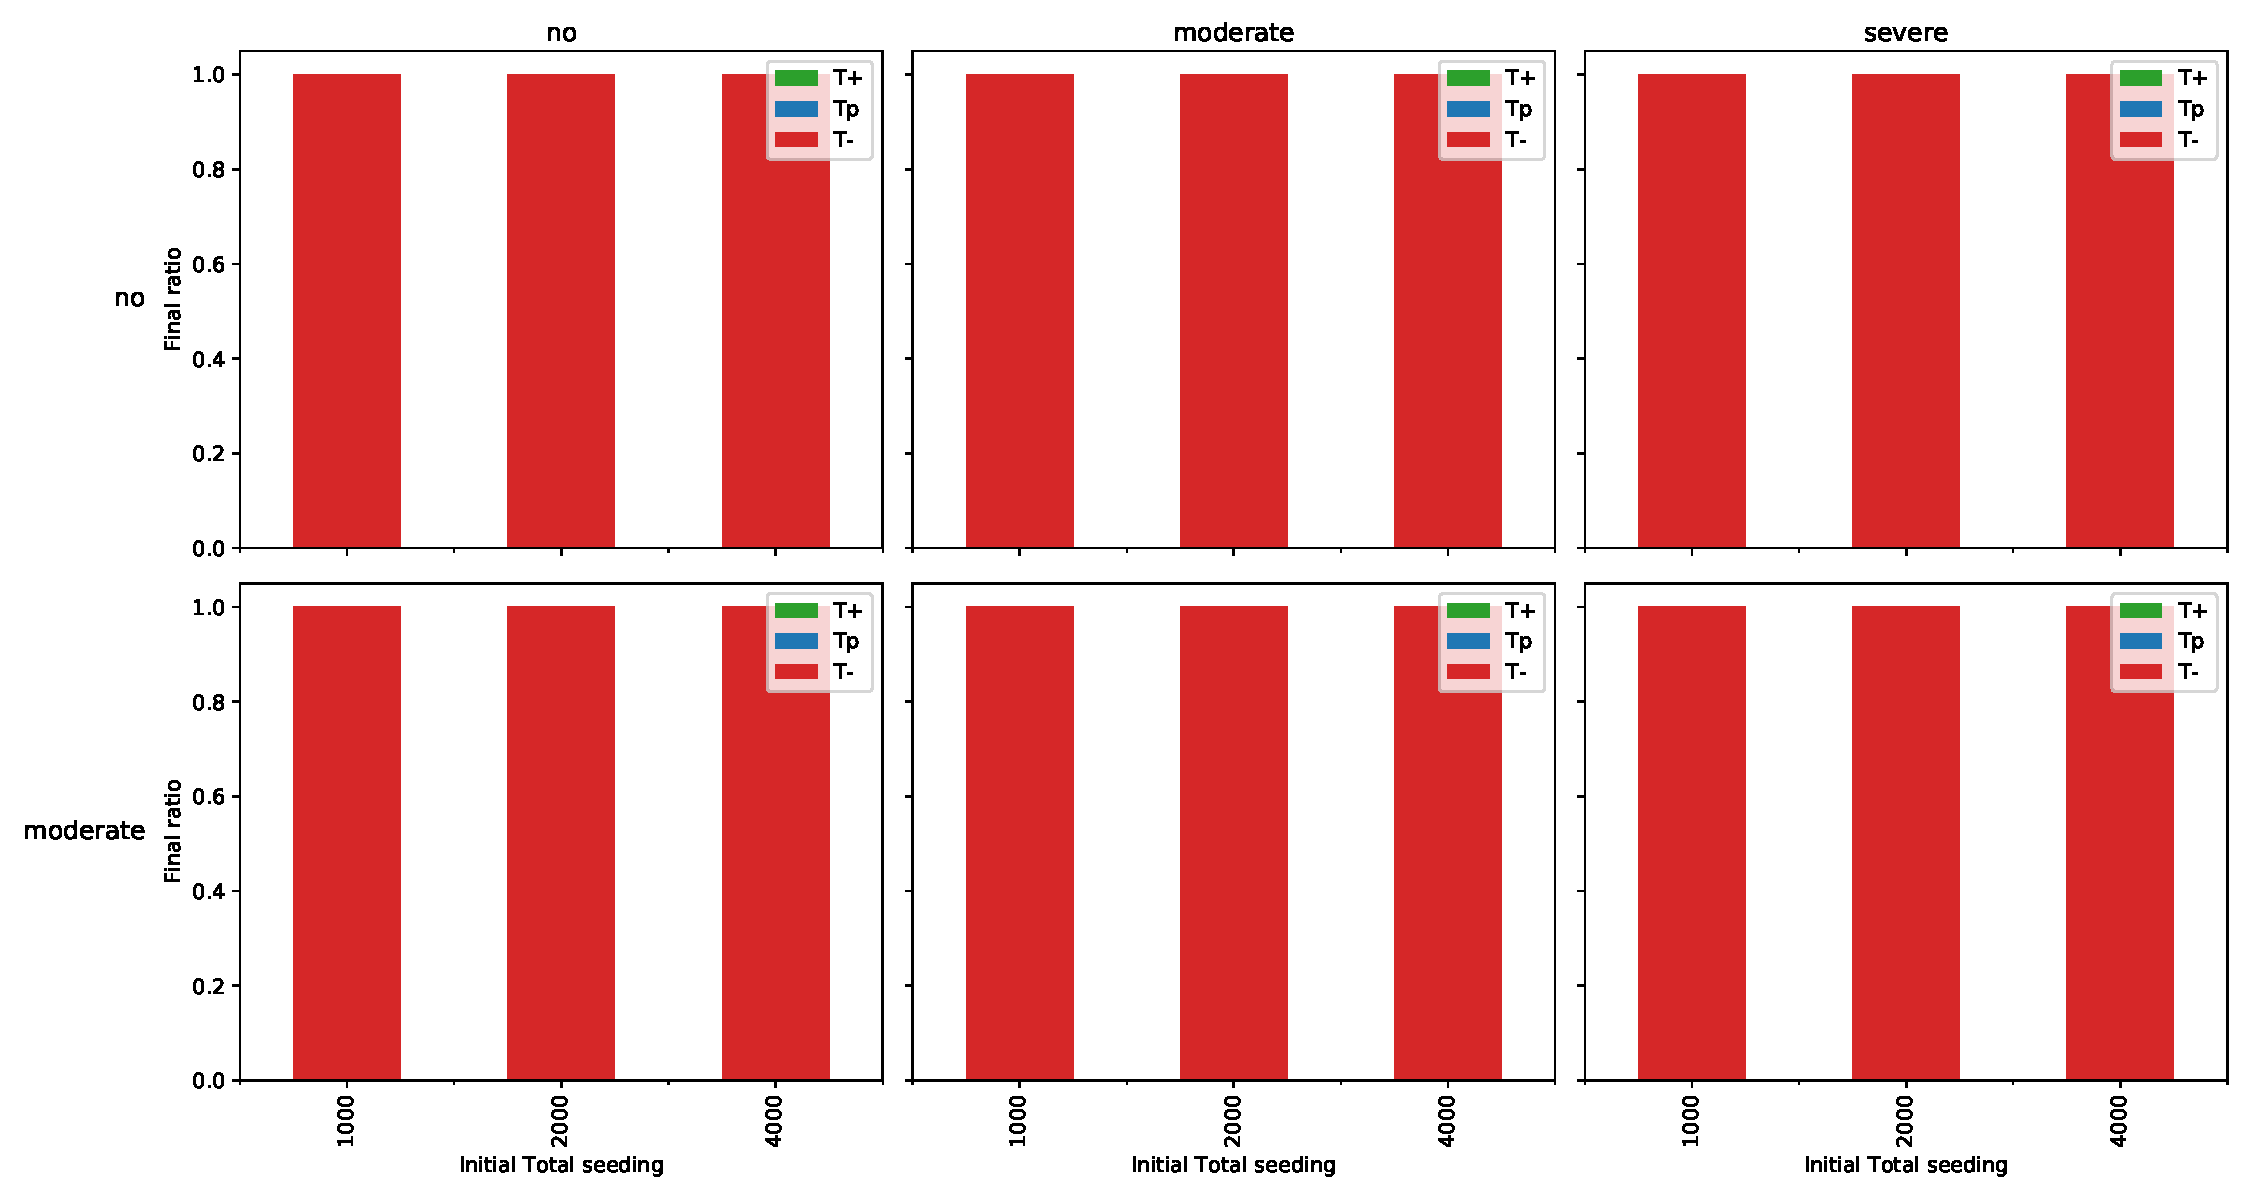
\includegraphics[width=\textwidth]{All3_therapy-SOC_1:1:1}
    \caption{Equal Seeding - $T^p:T^+:T^-$ :: 1:1:1}
    \label{fig_therapy-SOC_1:1:1}
  \end{subfigure}
  \begin{subfigure}[b]{\textwidth}
    \centering
    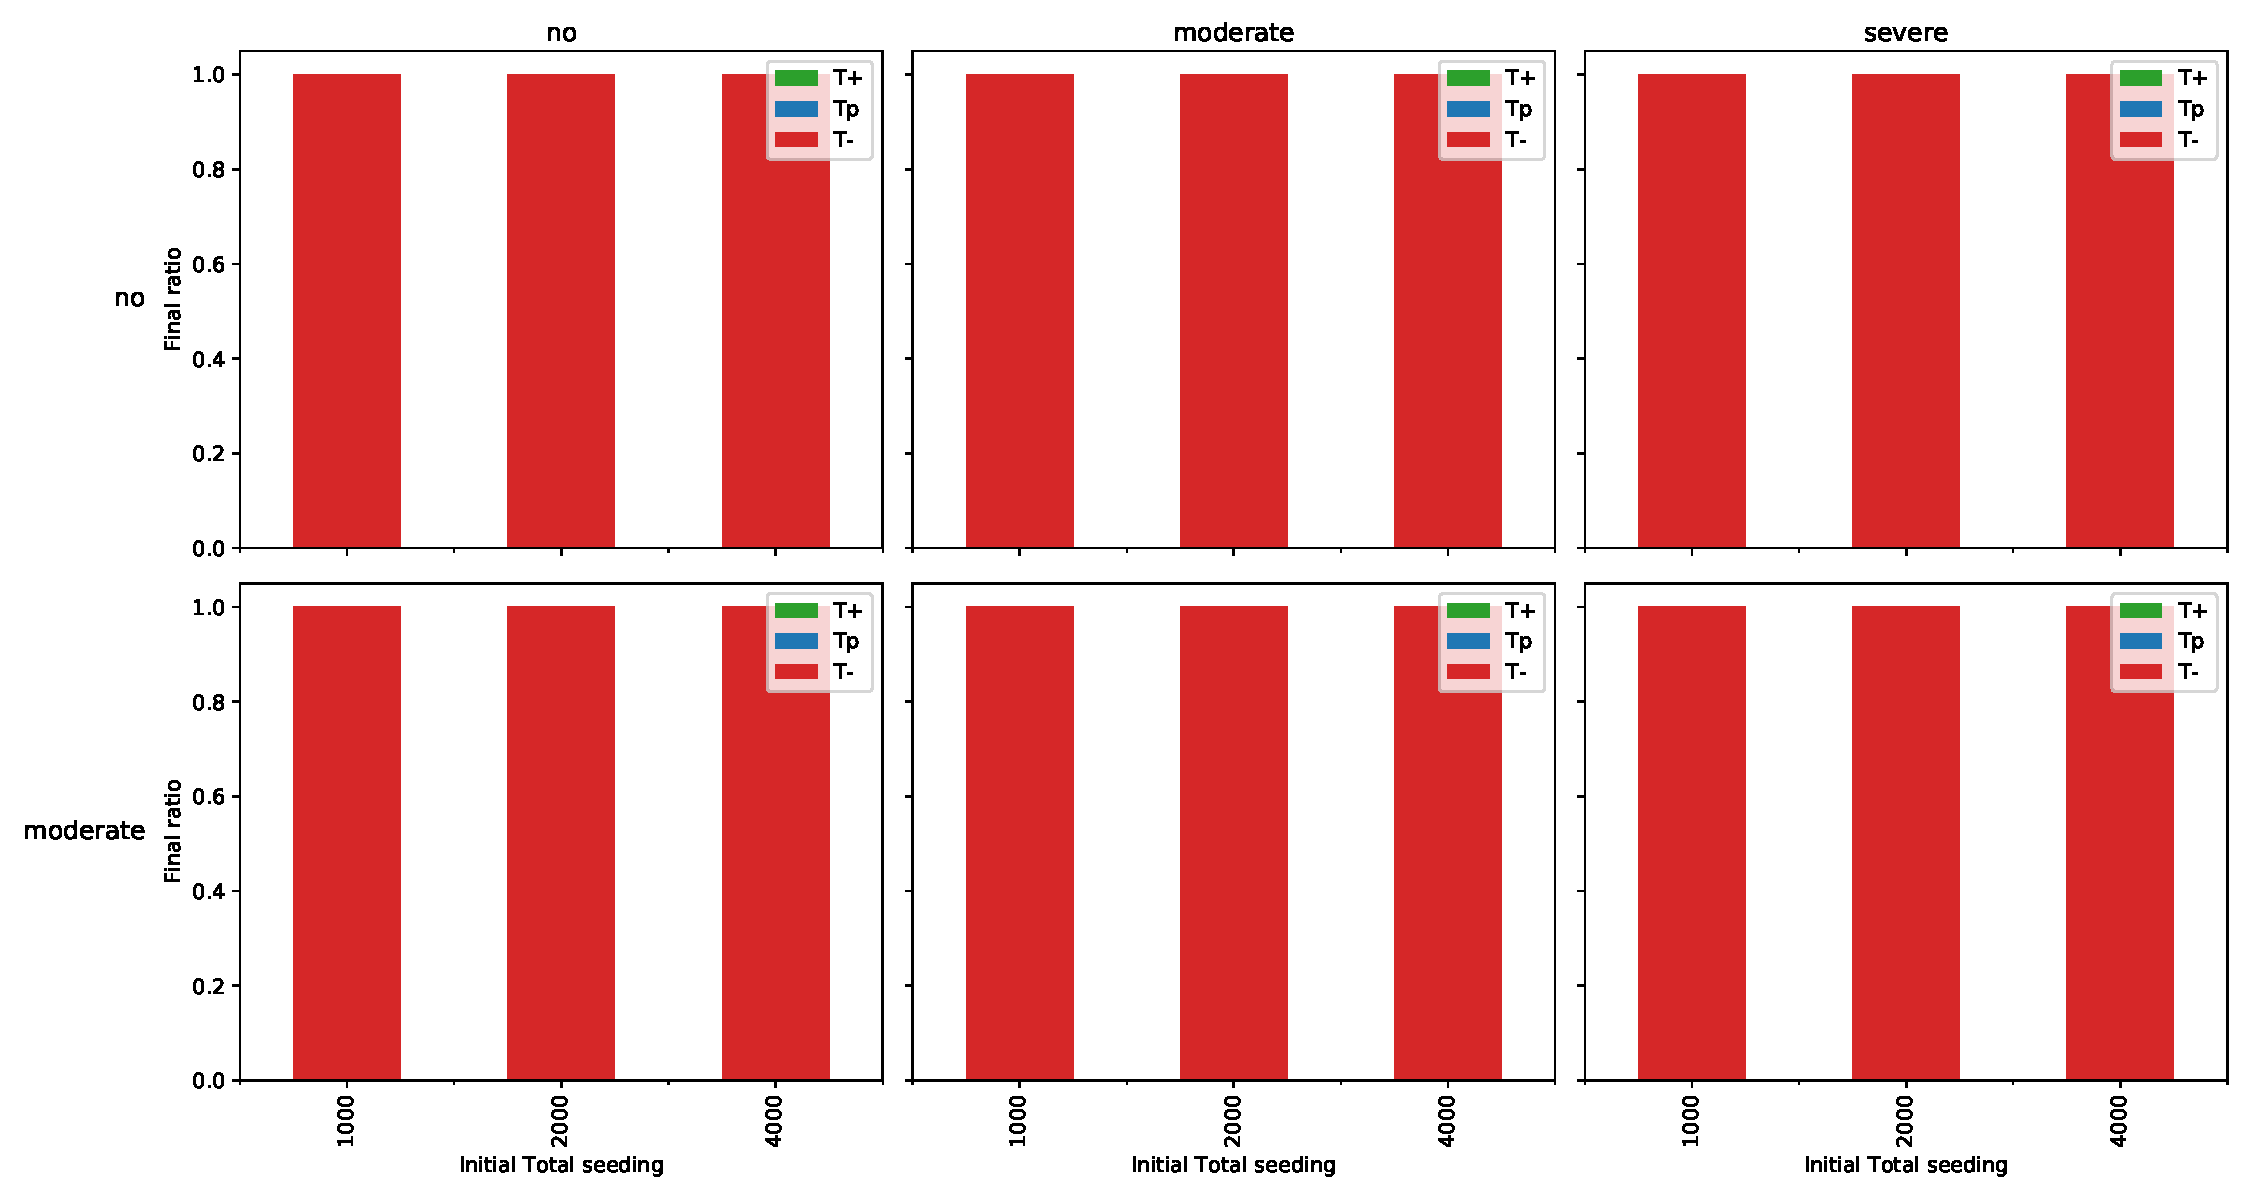
\includegraphics[width=\textwidth]{All3_therapy-SOC_8:1:1}
    \caption{High $T^p$ seeding- $T^p:T^+:T^-$ :: 8:1:1}
    \label{fig_therapy-SOC_8:1:1}
  \end{subfigure}
  \caption[Final ratio of all cell types under standard-of-care]{Final ratio of all cell types under standard-of-care under different oxygen limits of $T^-$ (columns), oxygen efficiencies of $T^+$, $T^p$ (rows) and initial seeding proportions, initial total seeding (subfigures).}
  \label{fig_therapy-SOC}
\end{figure}

\newpage

\section{Adaptive Therapy (AT)}
Implementation of adaptive therapy (AT) is based on thresholds of population size; the On threshold is the size above which therapy would be applied and the Off threshold is the size below which therapy would be withdrawn. A range of such size thresholds were tried out for the case where testosterone is not limiting and oxygen has low limitation. For the purposes of this model, abiraterone therapy thresholds were defined in terms of the population sizes of the hormone-dependent subpopulations alone, $T^+$ and $T^p$. There are some indications from the literature that distinguishing between hormone-dependent and -independent fractions of prostate cancer cells may be possible clinically based on levels of specific prostate-specific antigen (PSA) types secreted by each \cite{Takahashi}.

The following general observations could be made based on our exploration of population size thresholds, some of which are visualised in \autoref{fig_therapy-AT_standardization}.
\begin{enumerate}
  \item In the AT modelling literature, a $50\%$ rule is commonly-used where therapy is applied above the initial population and withdrawn below $50\%$ of that. In our exploration, we found that for low threshold sizes, the $T^p$ and $T^+$ populations are so low that competitive inhibition by $T^-$ drives them to extinction. This low threshold size was also found to include the population size range where the $50\%$ rule would operate, which casts some doubt on the effectiveness of this threshold.
  \item It follows directly from above that a higher threshold would be better for $T^p$ and $T^+$ to survive the competition by $T^-$ as well as to suppress $T^-$, while increased effectiveness of a higher threshold has also been shown elsewhere \cite{Hansen}. However, increasing the threshold close to the effective carrying capacity eventually leads to no therapy being applied for the entire simulation duration as the population sizes never cross the on threshold. While there may be some grounds for a clinical decision not to apply any treatment, such a situation is not suited for an exhaustive theoretical study of the factors affecting AT. The threshold of On:6000 and Off:4000 was therefore chosen for further exploration as a reasonable middle ground between competitive release and no therapy.
  \item As mentioned earlier, only $T^p$ and $T^+$ cell types were considered for the thresholds for therapy. For the sake of completeness, the case where all the three cell types are considered for the thresholds for therapy was also tried out as visualised in \autoref{fig_therapy-AT_standardization-Total}. However, all the cases led to competitive release in the initial few days, suggesting that total population size makes for a poorer cue for AT application and withdrawal.
\end{enumerate}

\begin{figure}[h!]
  \centering
  \begin{subfigure}[b]{\textwidth}
    \centering
    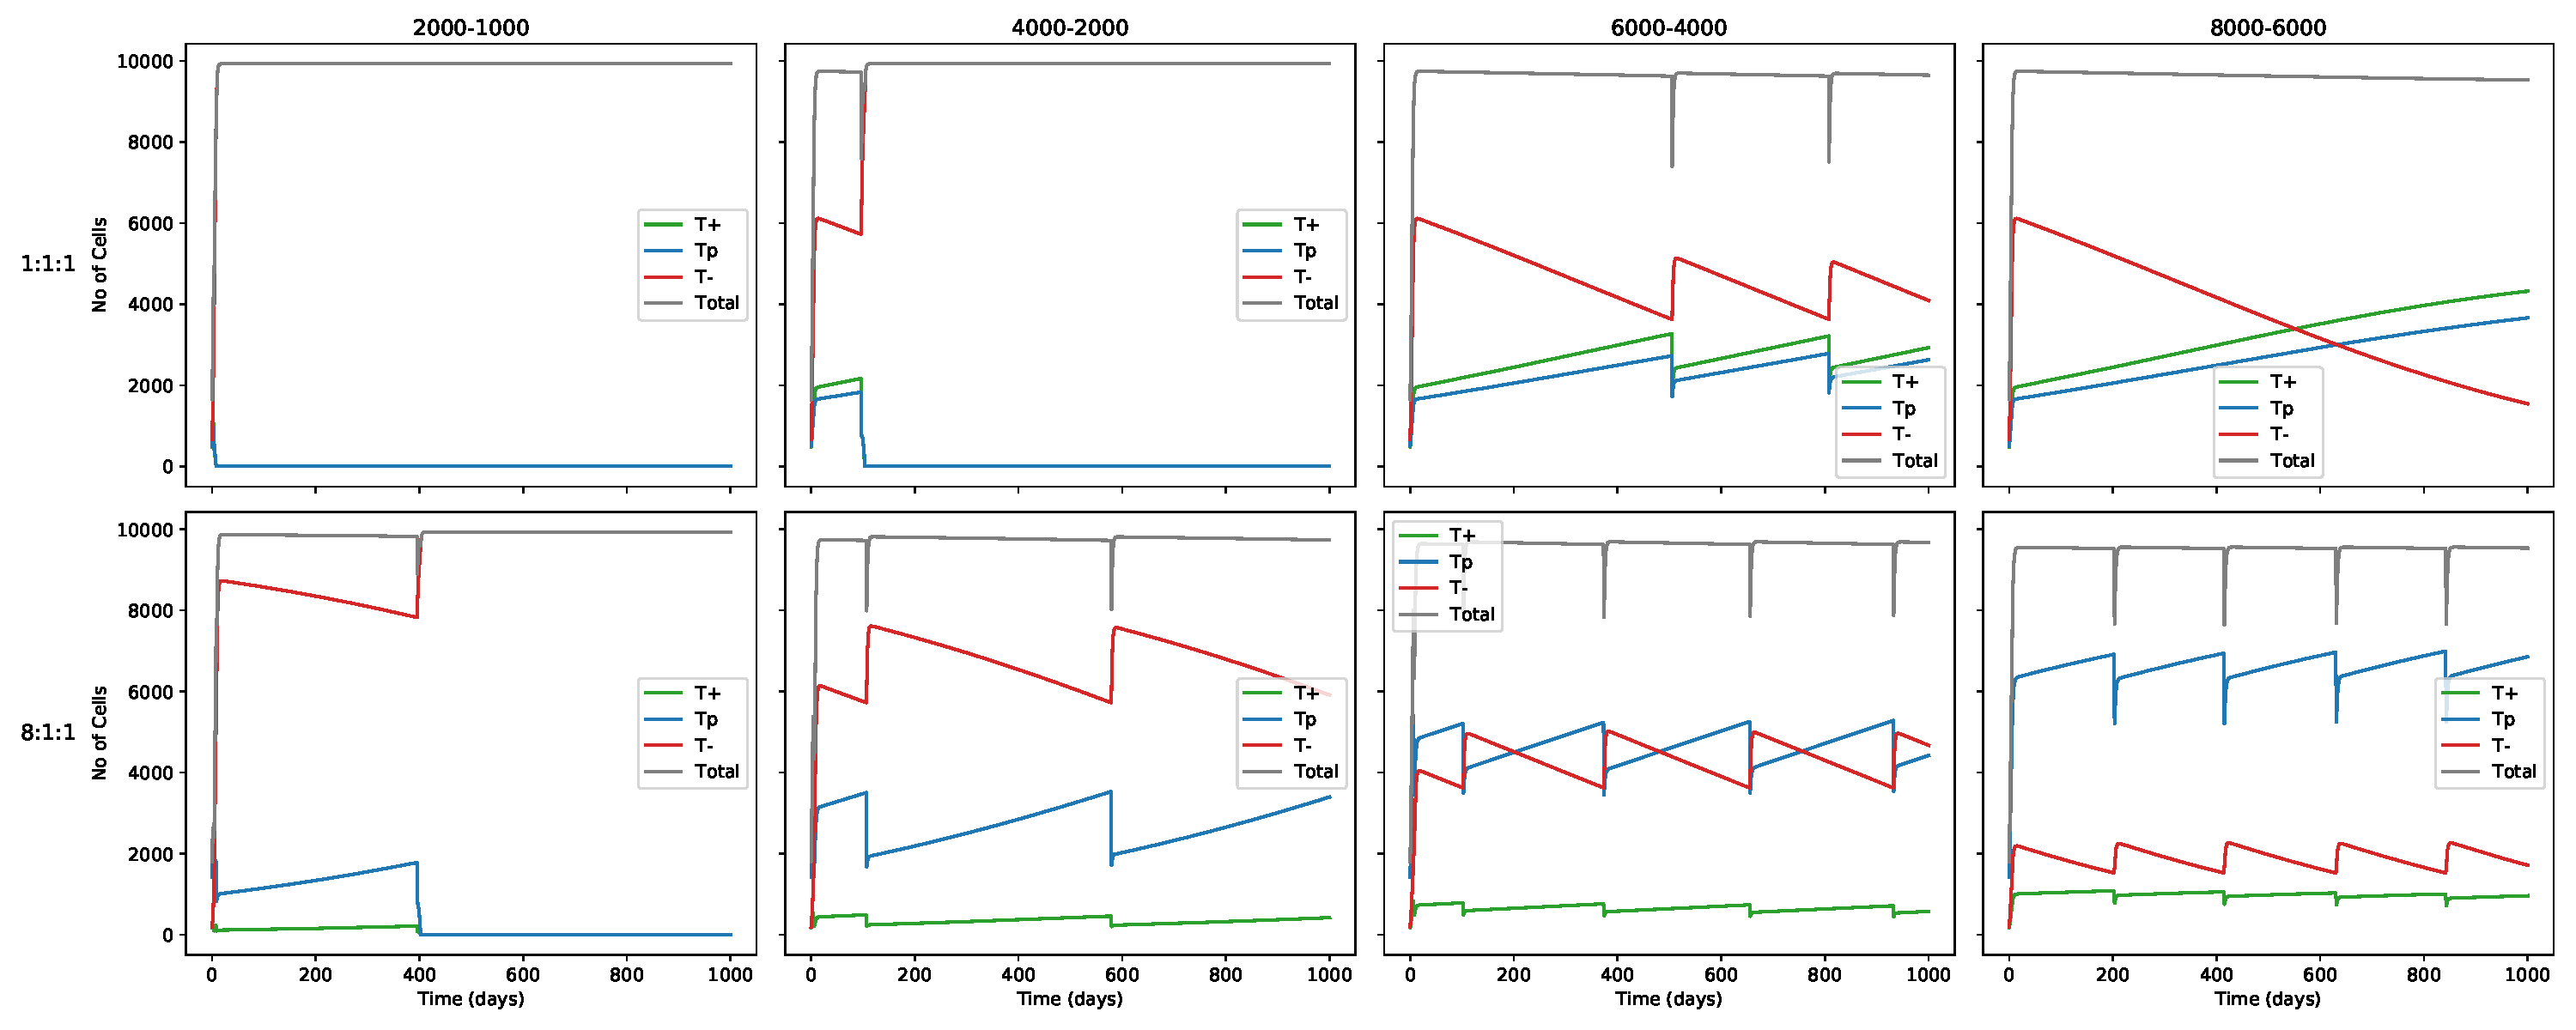
\includegraphics[width=\textwidth]{All3_therapy-standardization}
  \end{subfigure}
  \begin{subfigure}[b]{\textwidth}
    \centering
    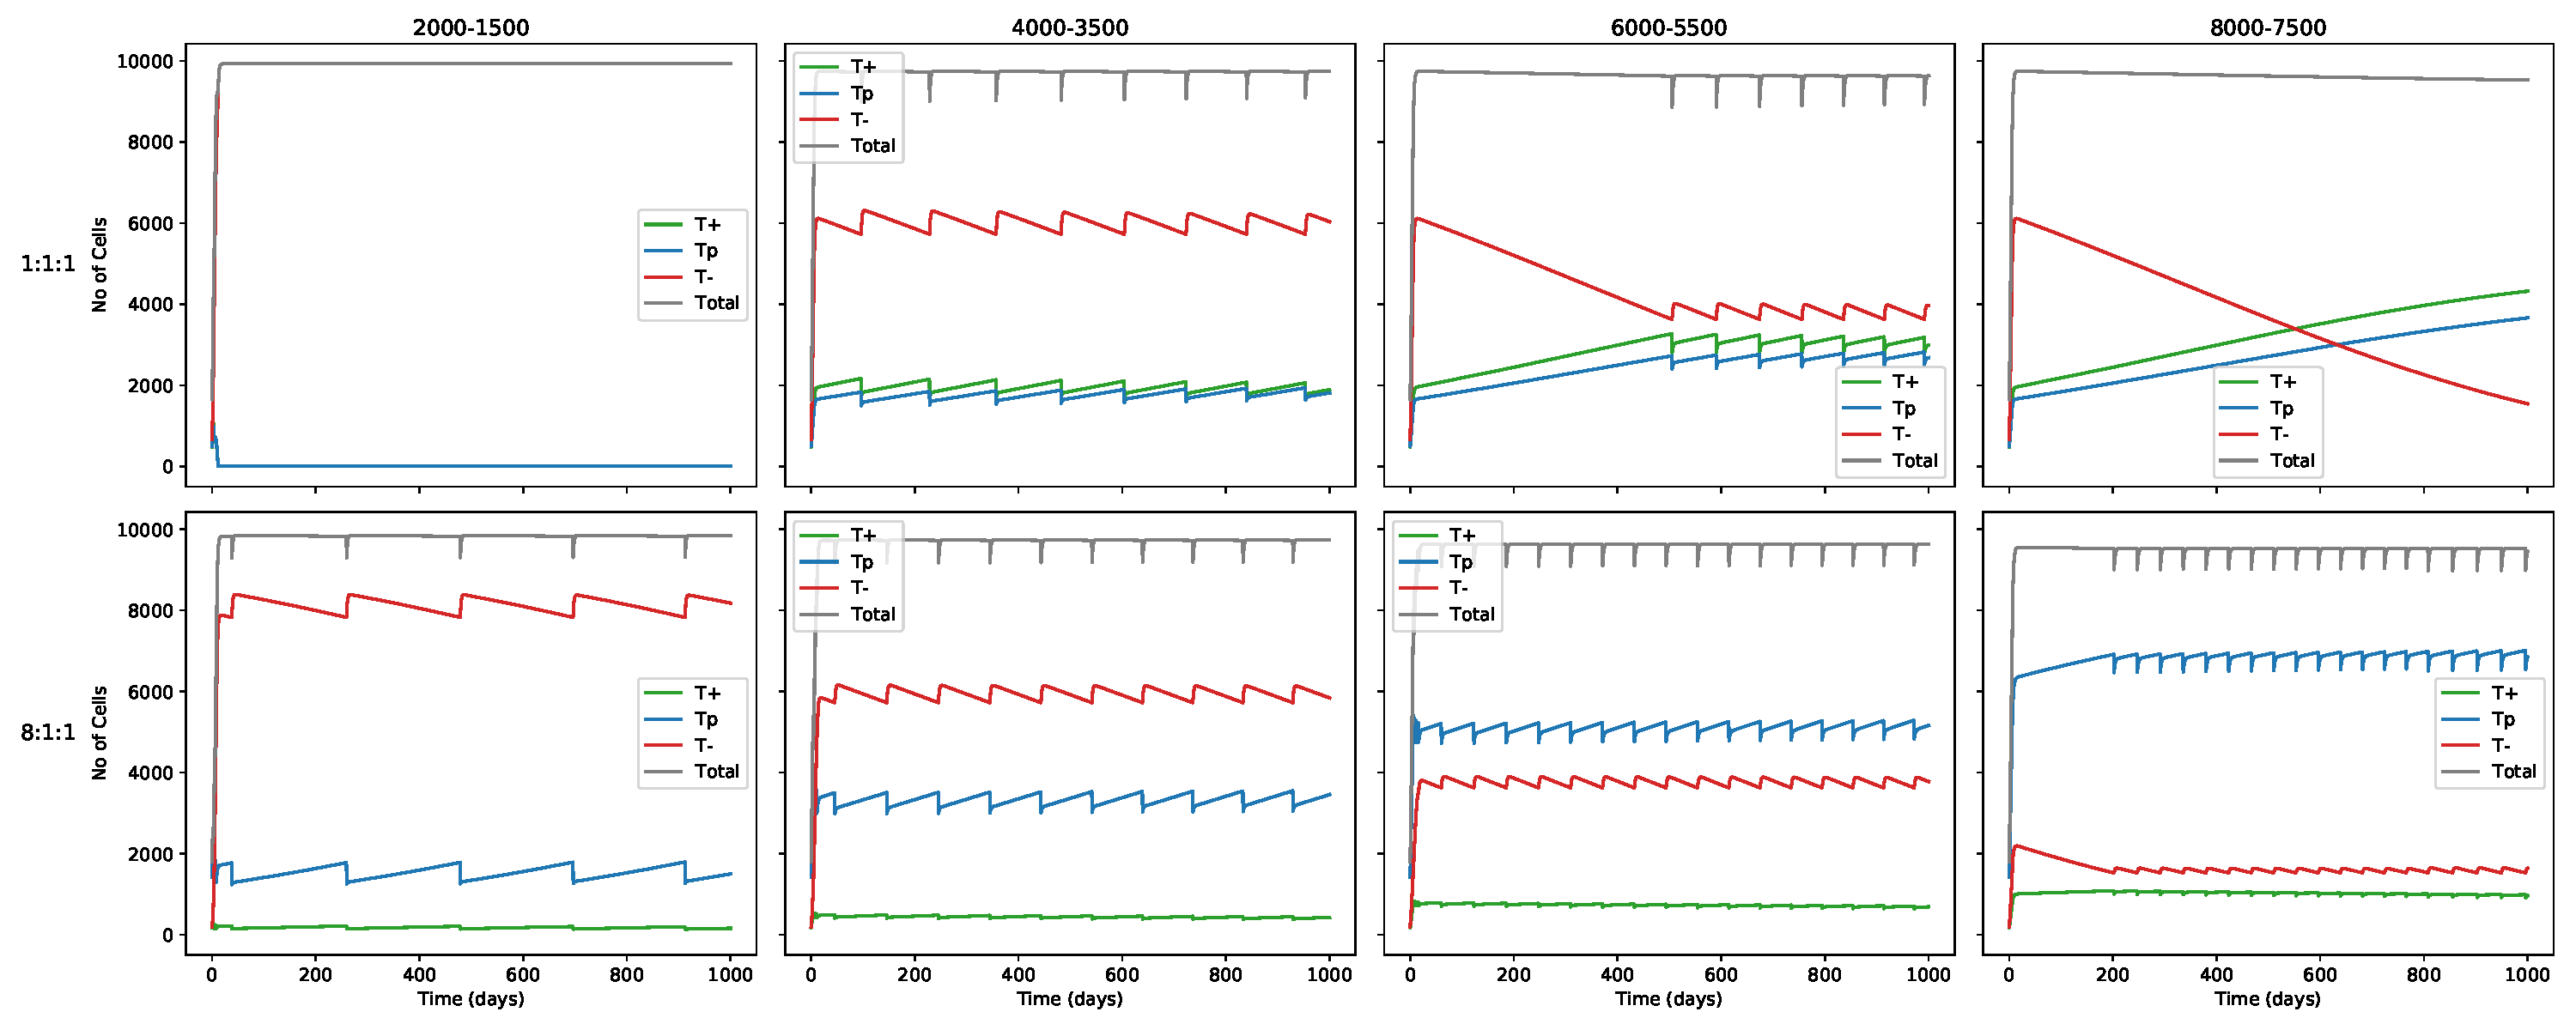
\includegraphics[width=\textwidth]{All3_therapy-standardization-sw}
  \end{subfigure}
  \caption[Standardisation of threshold for adaptive therapy]{Standardisation of threshold for adaptive therapy, Columns: On-Off threshold, Rows: $T^p:T^+:T^-$ Seeding}
  \label{fig_therapy-AT_standardization}
\end{figure}

\newpage

\subsection{Without delay}
With fixed On and Off thresholds of 6000 and 4000 respectively, AT was then applied systematically to every combination of resource limitation studied in the previous section. The results from these different cases are summarised below and visualised in \autoref{fig_therapy-AT}.
\begin{enumerate}
  \item Tumours with higher numbers of $T^p$ and $T^+$ would be more responsive to abiraterone and hence more treatable. Coexistence is of importance here as extinction of $T^p$ and $T^+$ would lead to no response.
  \item For cases when testosterone is moderately limiting and testosterone levels below the requirement of $T^p$ and $T^+$, these two cell types go extinct just by the competition from $T^-$ and produce no response from abiraterone naturally. Therefore, abiraterone efficacy depends strongly on $T^p$ seeding densities and total population, as with coexistence.
  \item In cases where coexistence is achieved, the $T^-$ cells quickly replace the space left by the dead $T^p$ and $T^+$ cells on applying therapy. In periods of no therapy, $T^p$ and $T^+$ cells compete with and replace the $T^-$ cells, but are soon met with therapy as they cross the on threshold. The total population size therefore remains high for most of the simulation, except when abiraterone is being applied where the $T^p$ population falls sharply. Despite this dip, the total population size recovers rapidly once therapy is withdrawn although there is some indication that total population size subsequently declines gradually until the next application, as $T^-$ cells are driven down by competition. Net decrease in the total population size itself, across multiple oscillations, is only seen in some combinations of resource limitation. In particular, this happens when testosterone is limiting (moderate limitation case) and/or the tumour population is still highly responsive to abiraterone (an active and considerable proportion of $T^p$ in the population), raising the possibility that even though AT, with a fixed window of treatment, outperforms SOC across the board, its effectiveness is modified strongly by the ecological state of the tumour population, in terms of cell type proportions and resource limitations.
\end{enumerate}

\begin{figure}[h!]
  \centering
  \begin{subfigure}[b]{\textwidth}
    \centering
    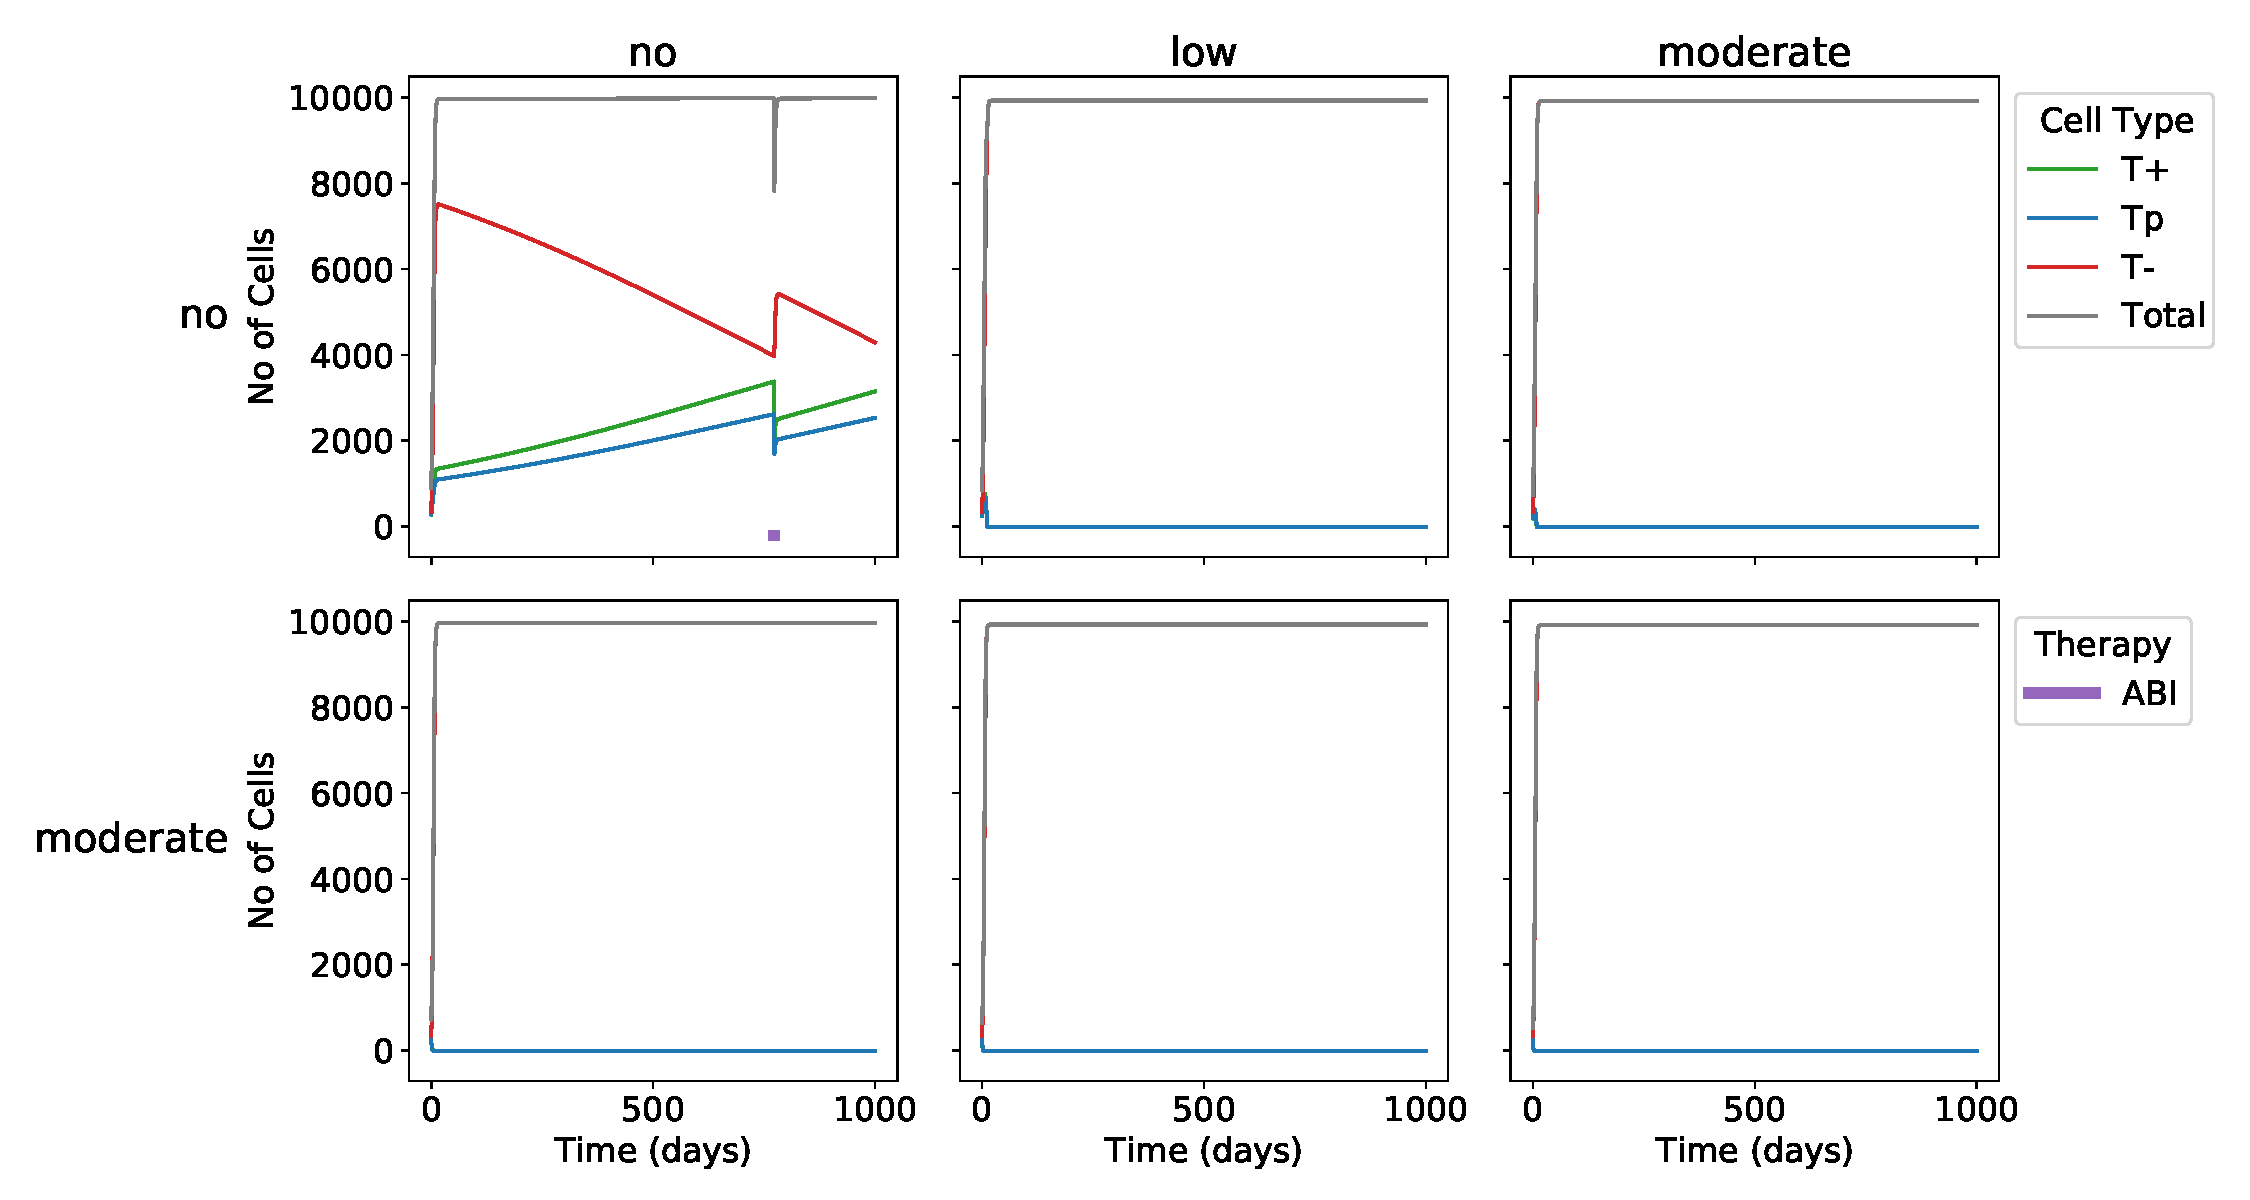
\includegraphics[width=\textwidth]{All3_therapy_1:1:1-1000}
    \caption{Equal Seeding - $T^p:T^+:T^-$ :: 1:1:1, Initial Total seeding: 1000}
    \label{fig_therapy-AT_1:1:1-1000}
  \end{subfigure}
  \begin{subfigure}[b]{\textwidth}
    \centering
    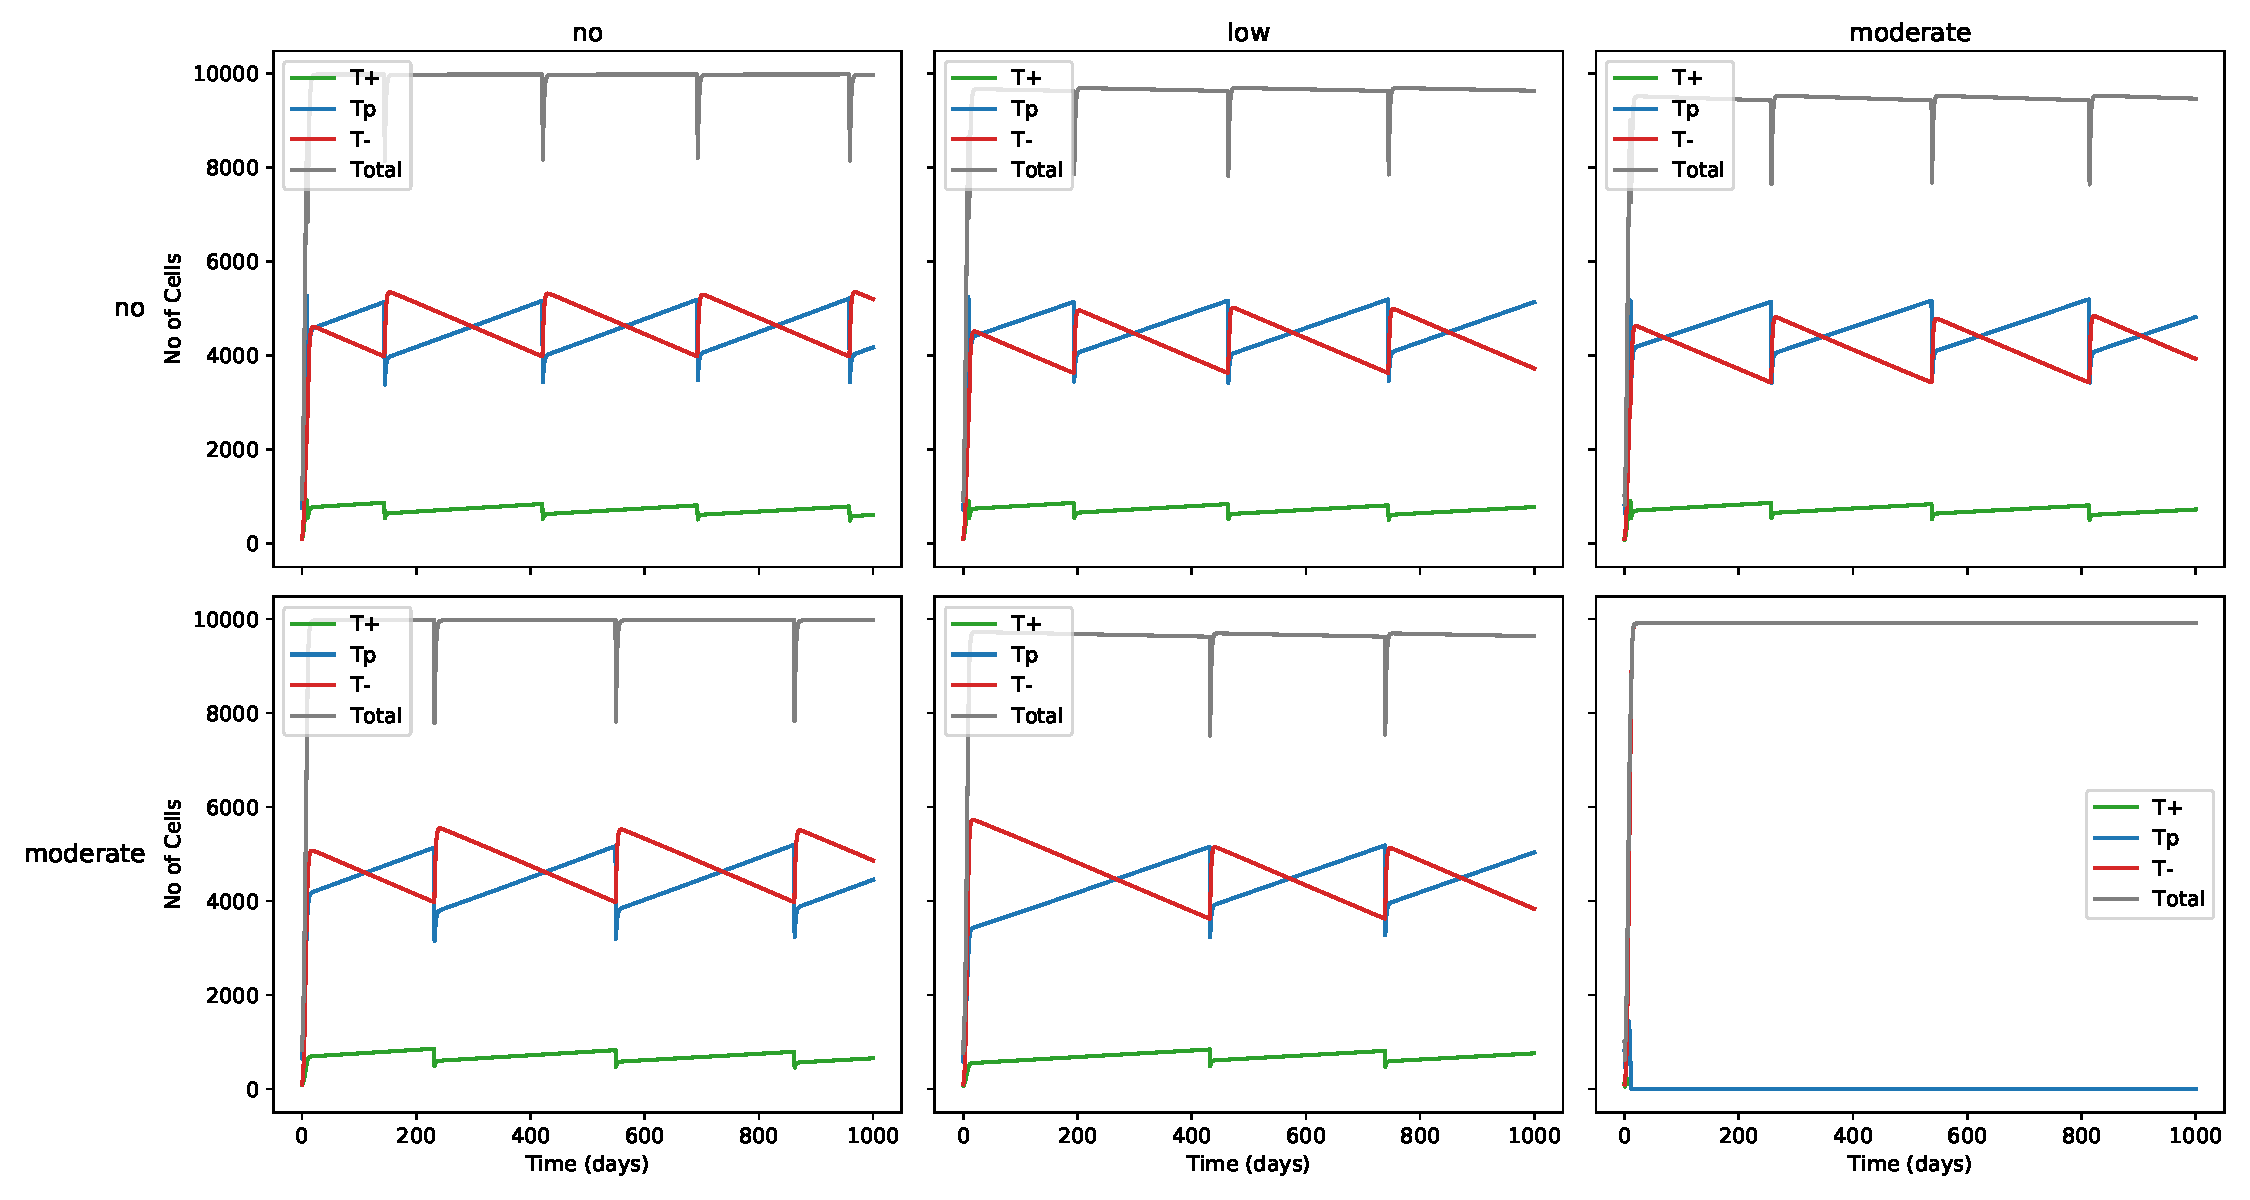
\includegraphics[width=\textwidth]{All3_therapy_8:1:1-1000}
    \caption{High $T^p$ seeding- $T^p:T^+:T^-$ :: 8:1:1, Initial Total seeding: 1000}
    \label{fig_therapy-AT_8:1:1-1000}
  \end{subfigure}
  \caption[]{(Continued on next page)}
\end{figure}
\begin{figure}[h!]\ContinuedFloat
  \centering
  \begin{subfigure}[b]{\textwidth}
    \centering
    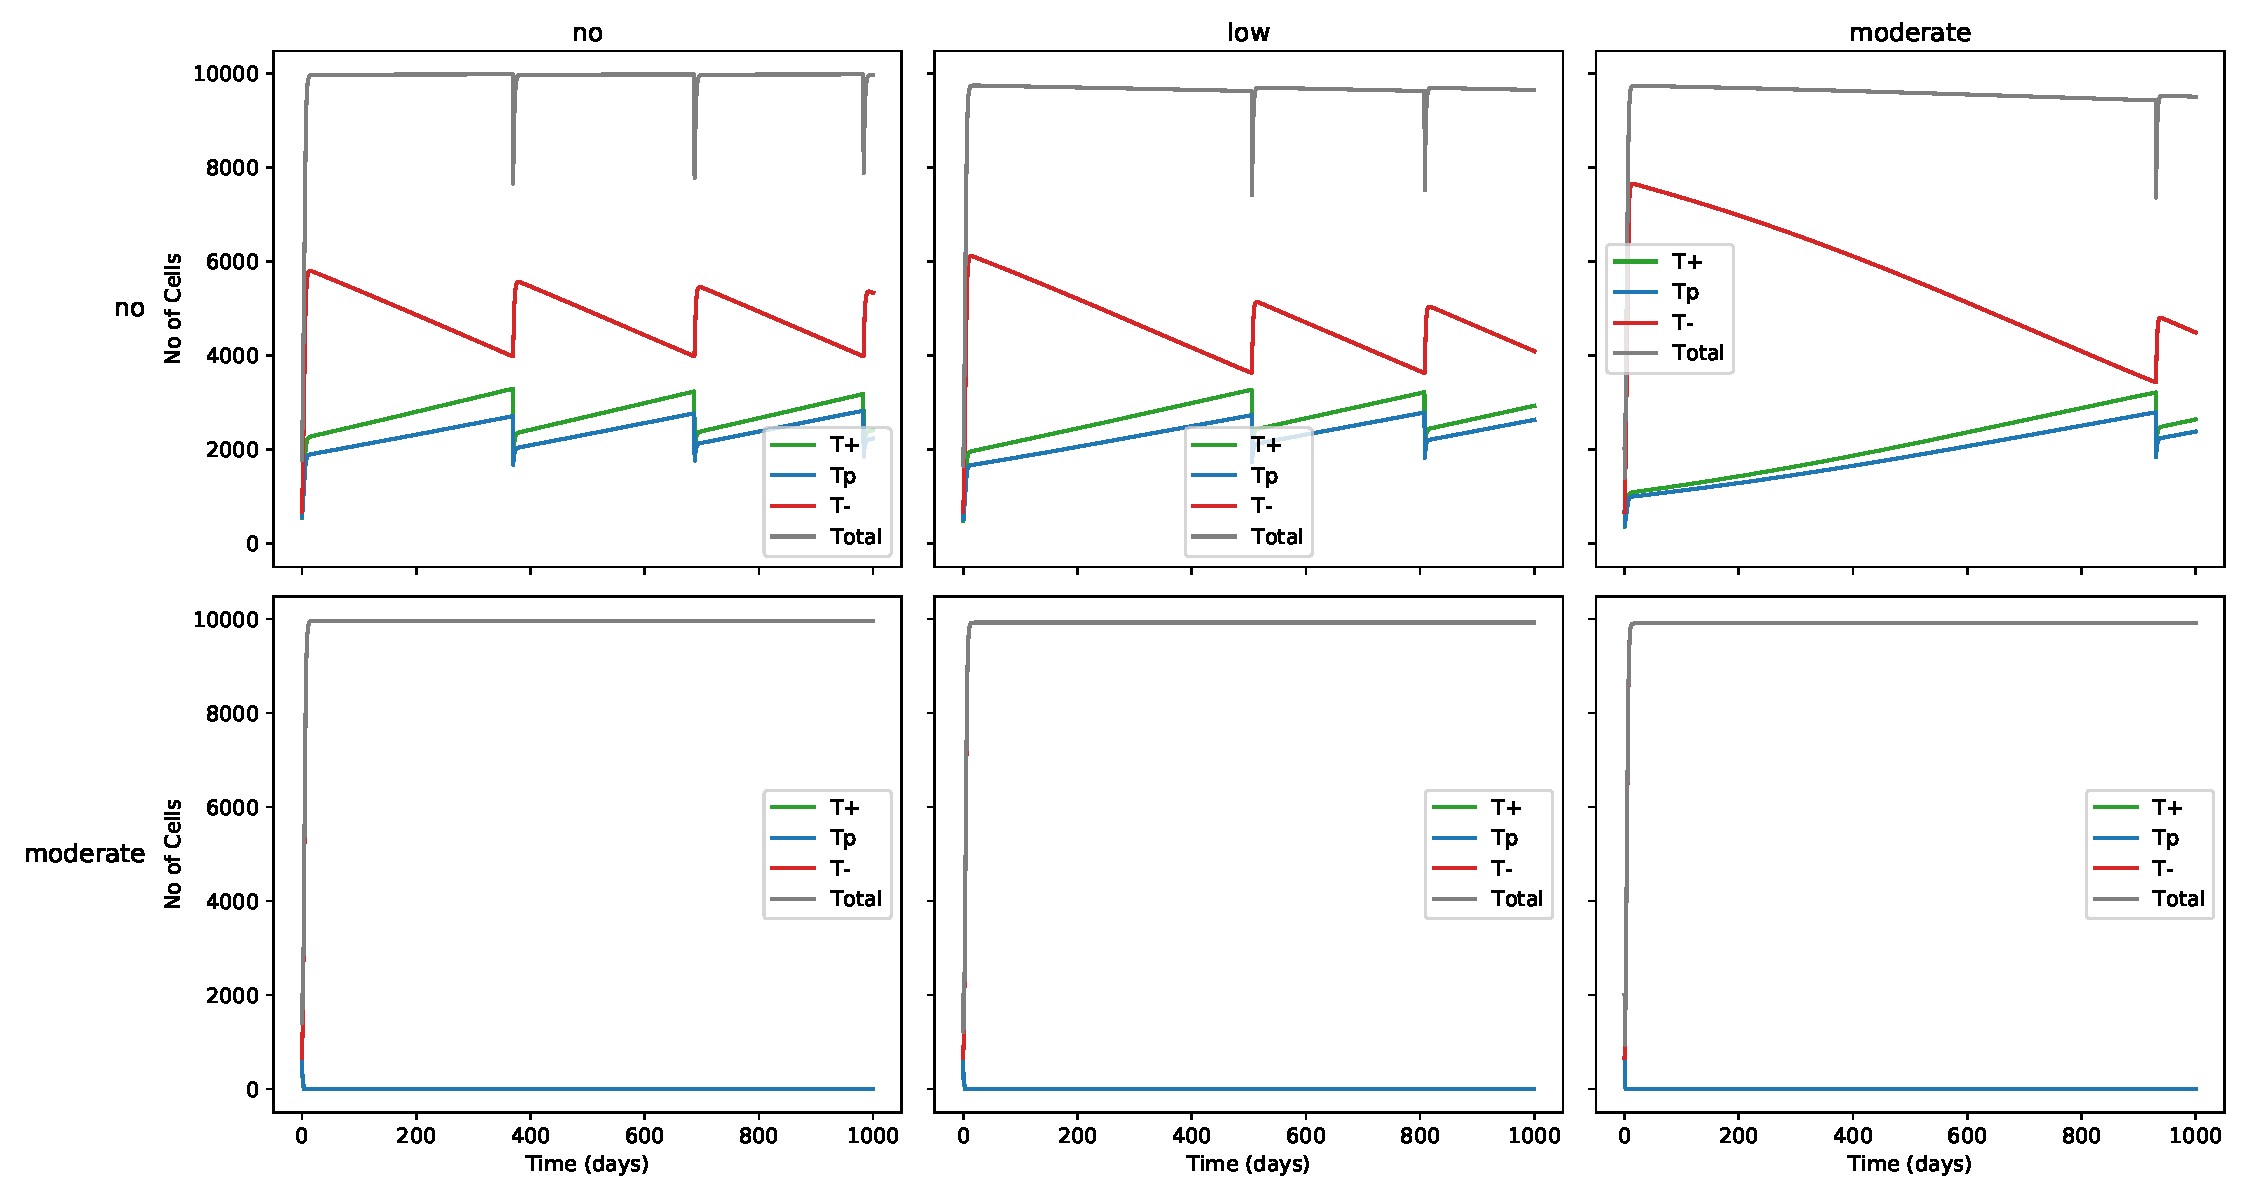
\includegraphics[width=\textwidth]{All3_therapy_1:1:1-2000}
    \caption{Equal Seeding - $T^p:T^+:T^-$ :: 1:1:1, Initial Total seeding: 2000}
    \label{fig_therapy-AT_1:1:1-2000}
  \end{subfigure}
  \begin{subfigure}[b]{\textwidth}
    \centering
    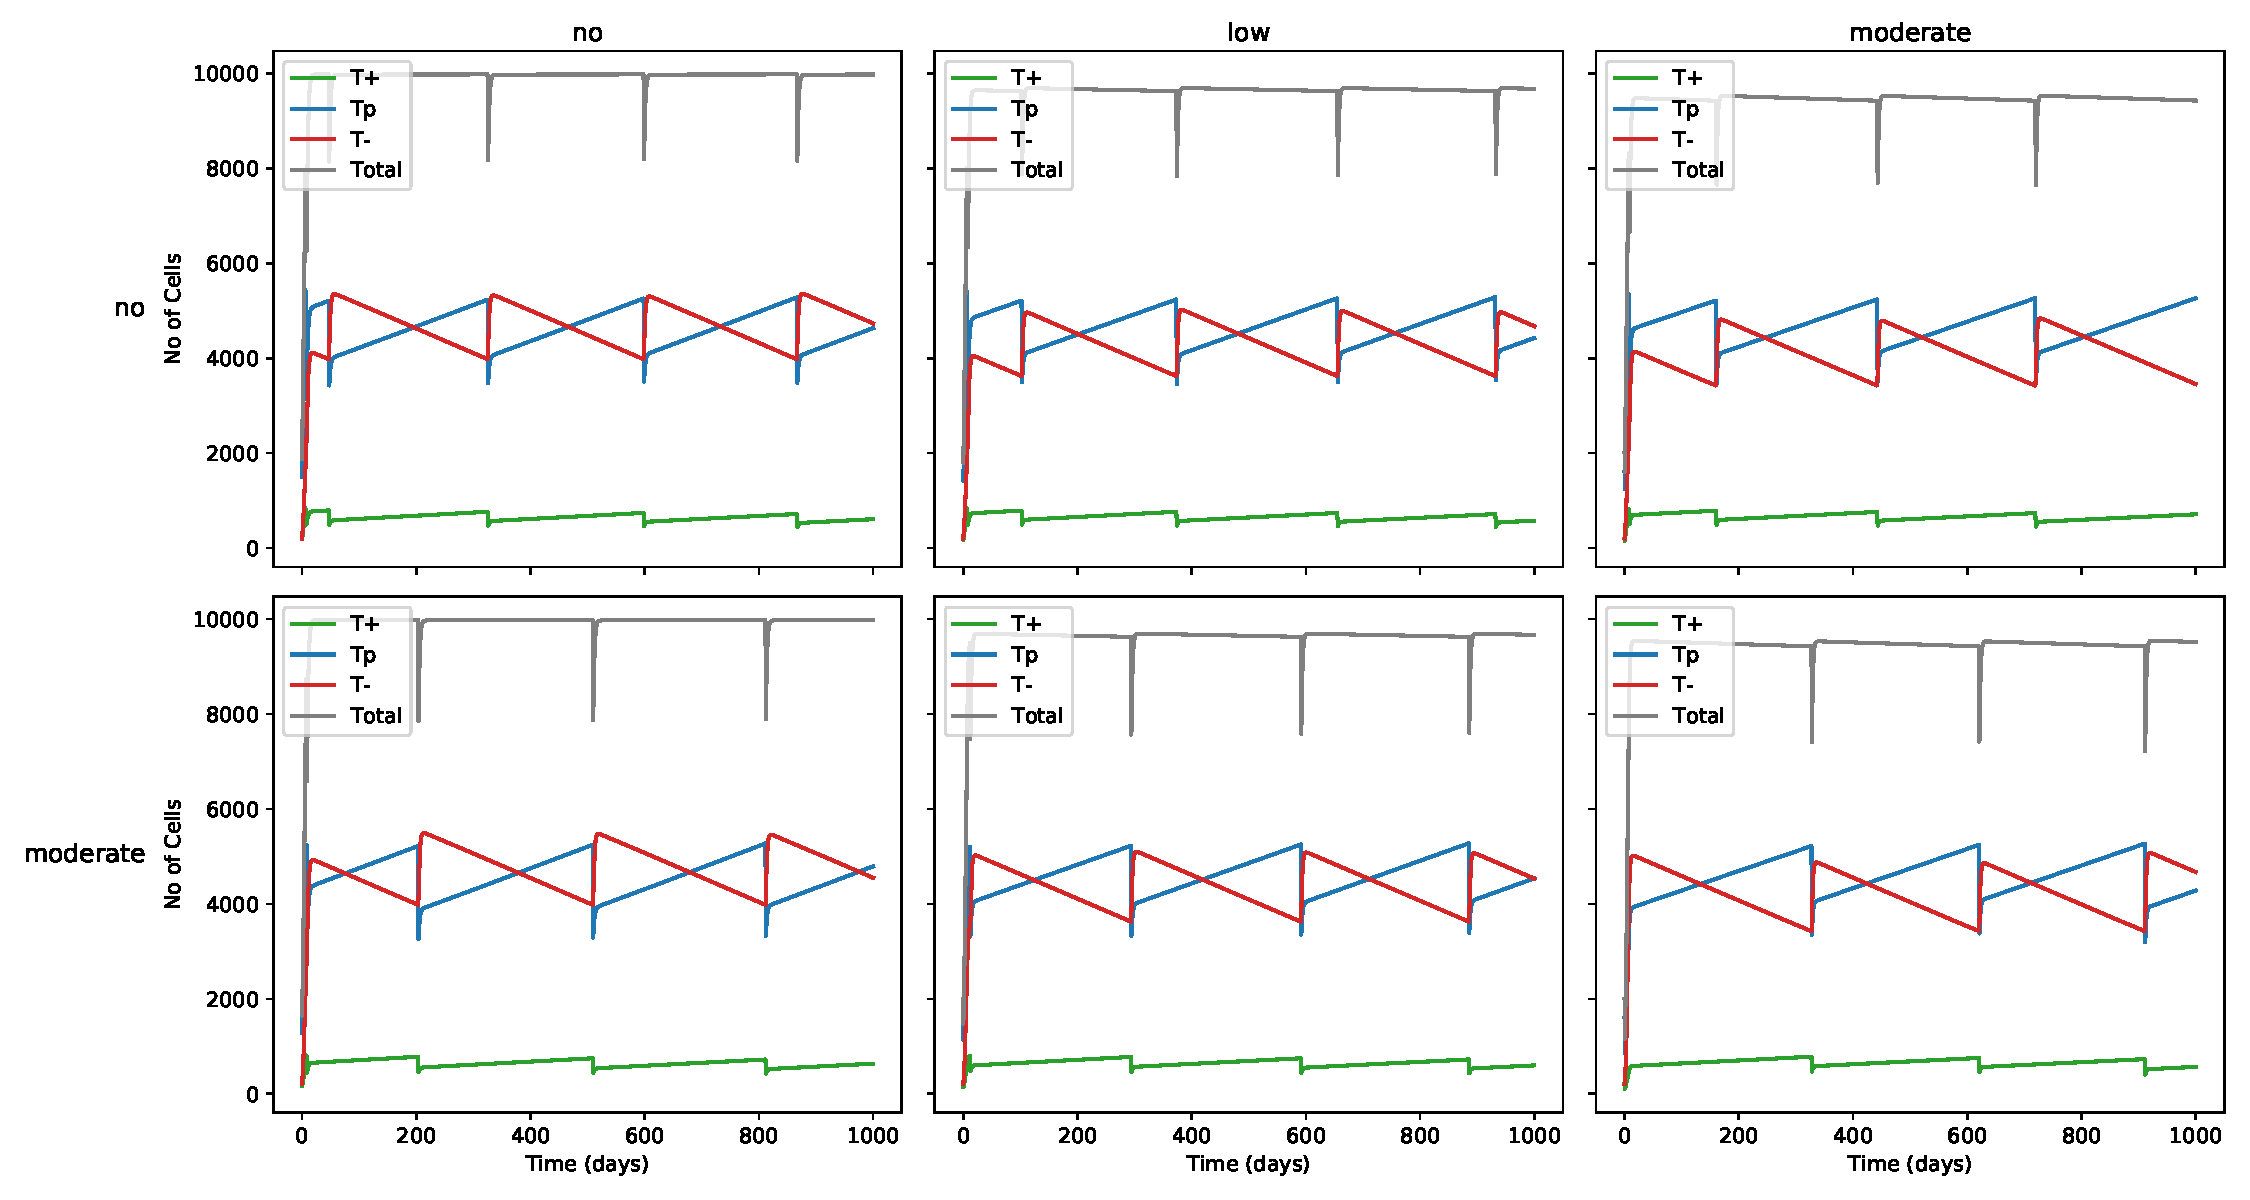
\includegraphics[width=\textwidth]{All3_therapy_8:1:1-2000}
    \caption{High $T^p$ seeding- $T^p:T^+:T^-$ :: 8:1:1, Initial Total seeding: 2000}
    \label{fig_therapy-AT_8:1:1-2000}
  \end{subfigure}
  \caption[]{(Continued on next page)}
\end{figure}
\begin{figure}[h!]\ContinuedFloat
  \centering
  \begin{subfigure}[b]{\textwidth}
    \centering
    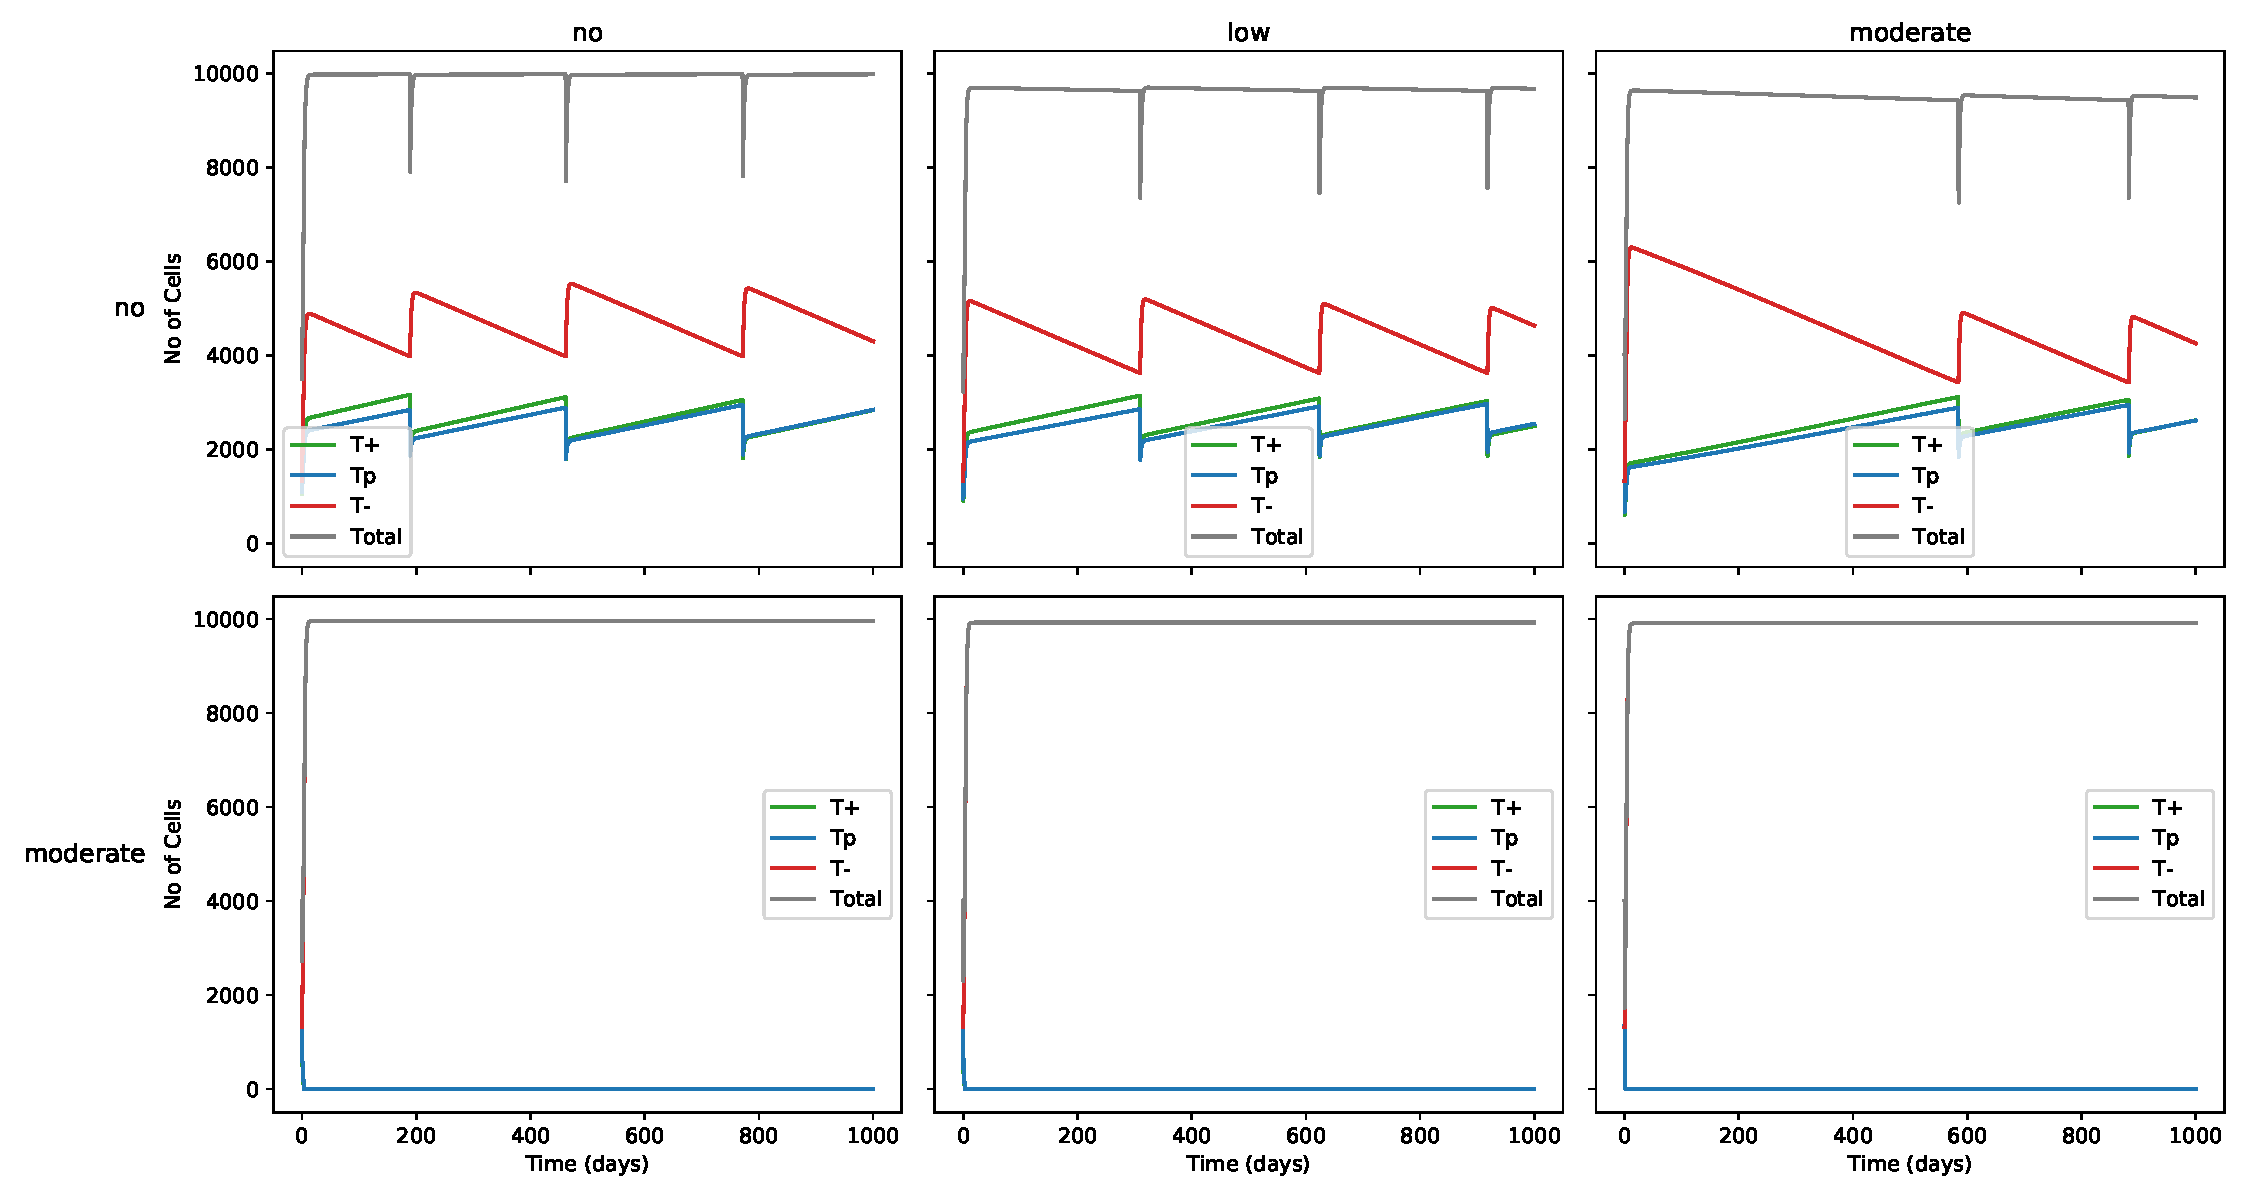
\includegraphics[width=\textwidth]{All3_therapy_1:1:1-4000}
    \caption{Equal Seeding - $T^p:T^+:T^-$ :: 1:1:1, Initial Total seeding: 4000}
    \label{fig_therapy-AT_1:1:1-4000}
  \end{subfigure}
  \begin{subfigure}[b]{\textwidth}
    \centering
    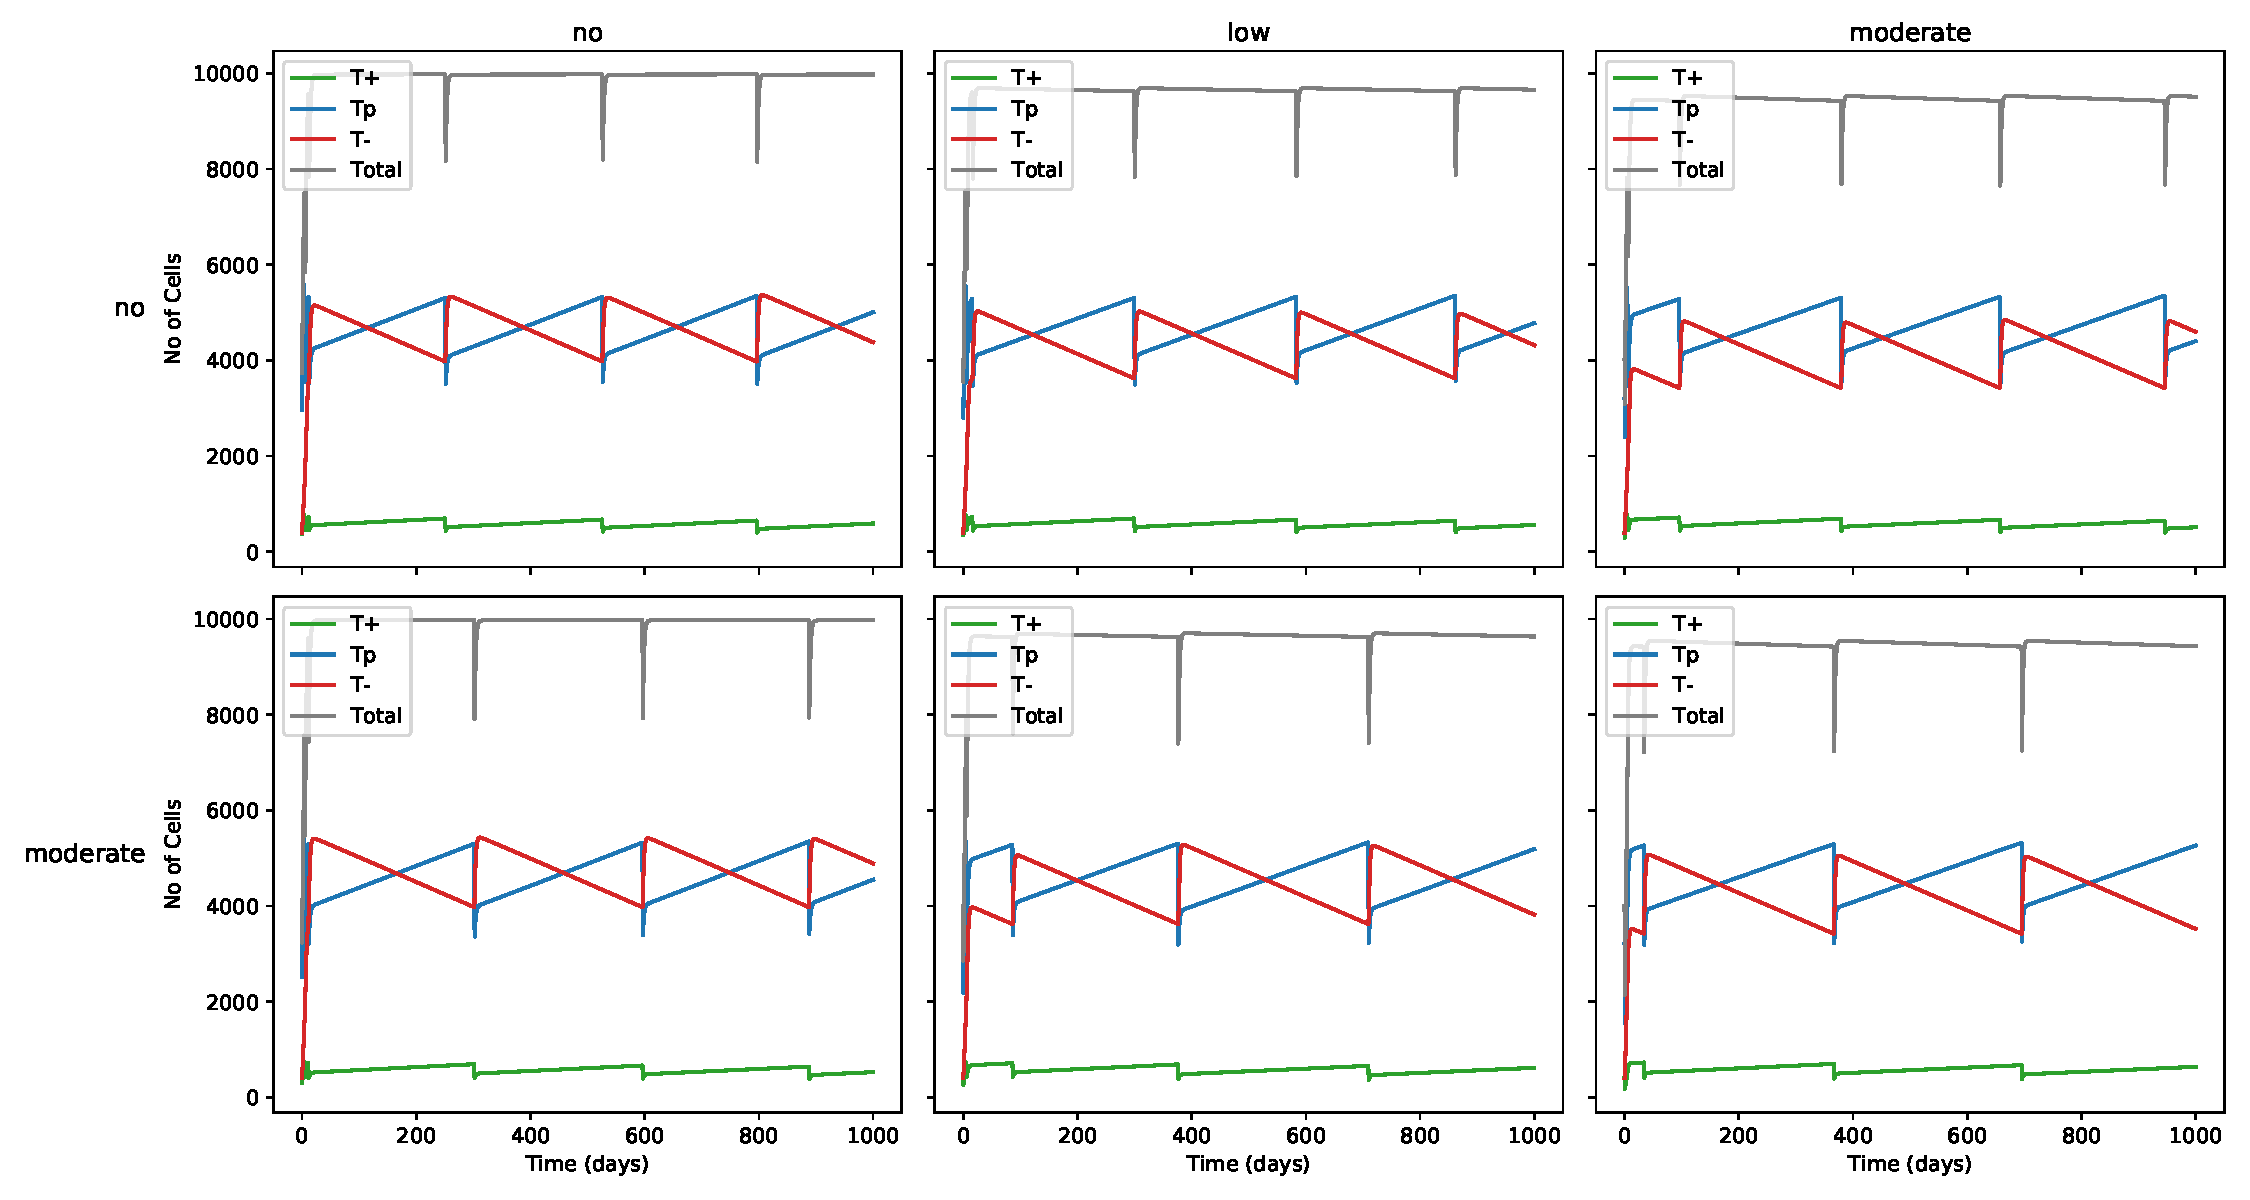
\includegraphics[width=\textwidth]{All3_therapy_8:1:1-4000}
    \caption{High $T^p$ seeding- $T^p:T^+:T^-$ :: 8:1:1, Initial Total seeding: 4000}
    \label{fig_therapy-AT_8:1:1-4000}
  \end{subfigure}
  \caption[Time-series of all cell types with adaptive therapy]{Time-series of all cell types with adaptive therapy (On:6000, Off:4000) under different oxygen limitation (columns), testosterone limitation (rows) and initial seeding proportions, initial total seeding (subfigures).}
  \label{fig_therapy-AT}
\end{figure}

\clearpage

\subsection{With delay}
As noted earlier, higher the amount of available testosterone, weaker the interspecific competition relative to intraspecific competition and therefore, better the coexistence. Since coexistence is tied strongly to the effectiveness of therapeutic outcomes, it stands to reason that the window of population sizes of $T^p$ and $T^+$ used in adaptive therapy be chosen to allow for sufficient numbers of $T^p$ and $T^+$ to remain in the population. Applying this idea specifically to the case with no limitation for either oxygen or testosterone, $T^p$ and $T^+$ population fractions increase monotonously with time even without treatment. It is therefore possible that early treatment could be detrimental to coexistence by causing early competitive release of $T^-$, and it is tempting to speculate whether delaying the onset of treatment could improve therapeutic outcomes by allowing for a better balance of $T^p - T^+$ and $T^-$. However, the conditions that we have tested here, shown in \autoref{fig_therapy-AT-delay}, do not show such an advantage to delay, possibly because we do not see much variability in the population fractions of each cell type within the delay time periods considered here. It is also important to note that this idea of delayed treatment does not account for the physiological cost of maintaining a growing tumour population until treatment is administered, which would be very important in a clinical setting.

\begin{figure}[h!]
  \centering
  \begin{subfigure}[b]{\textwidth}
    \centering
    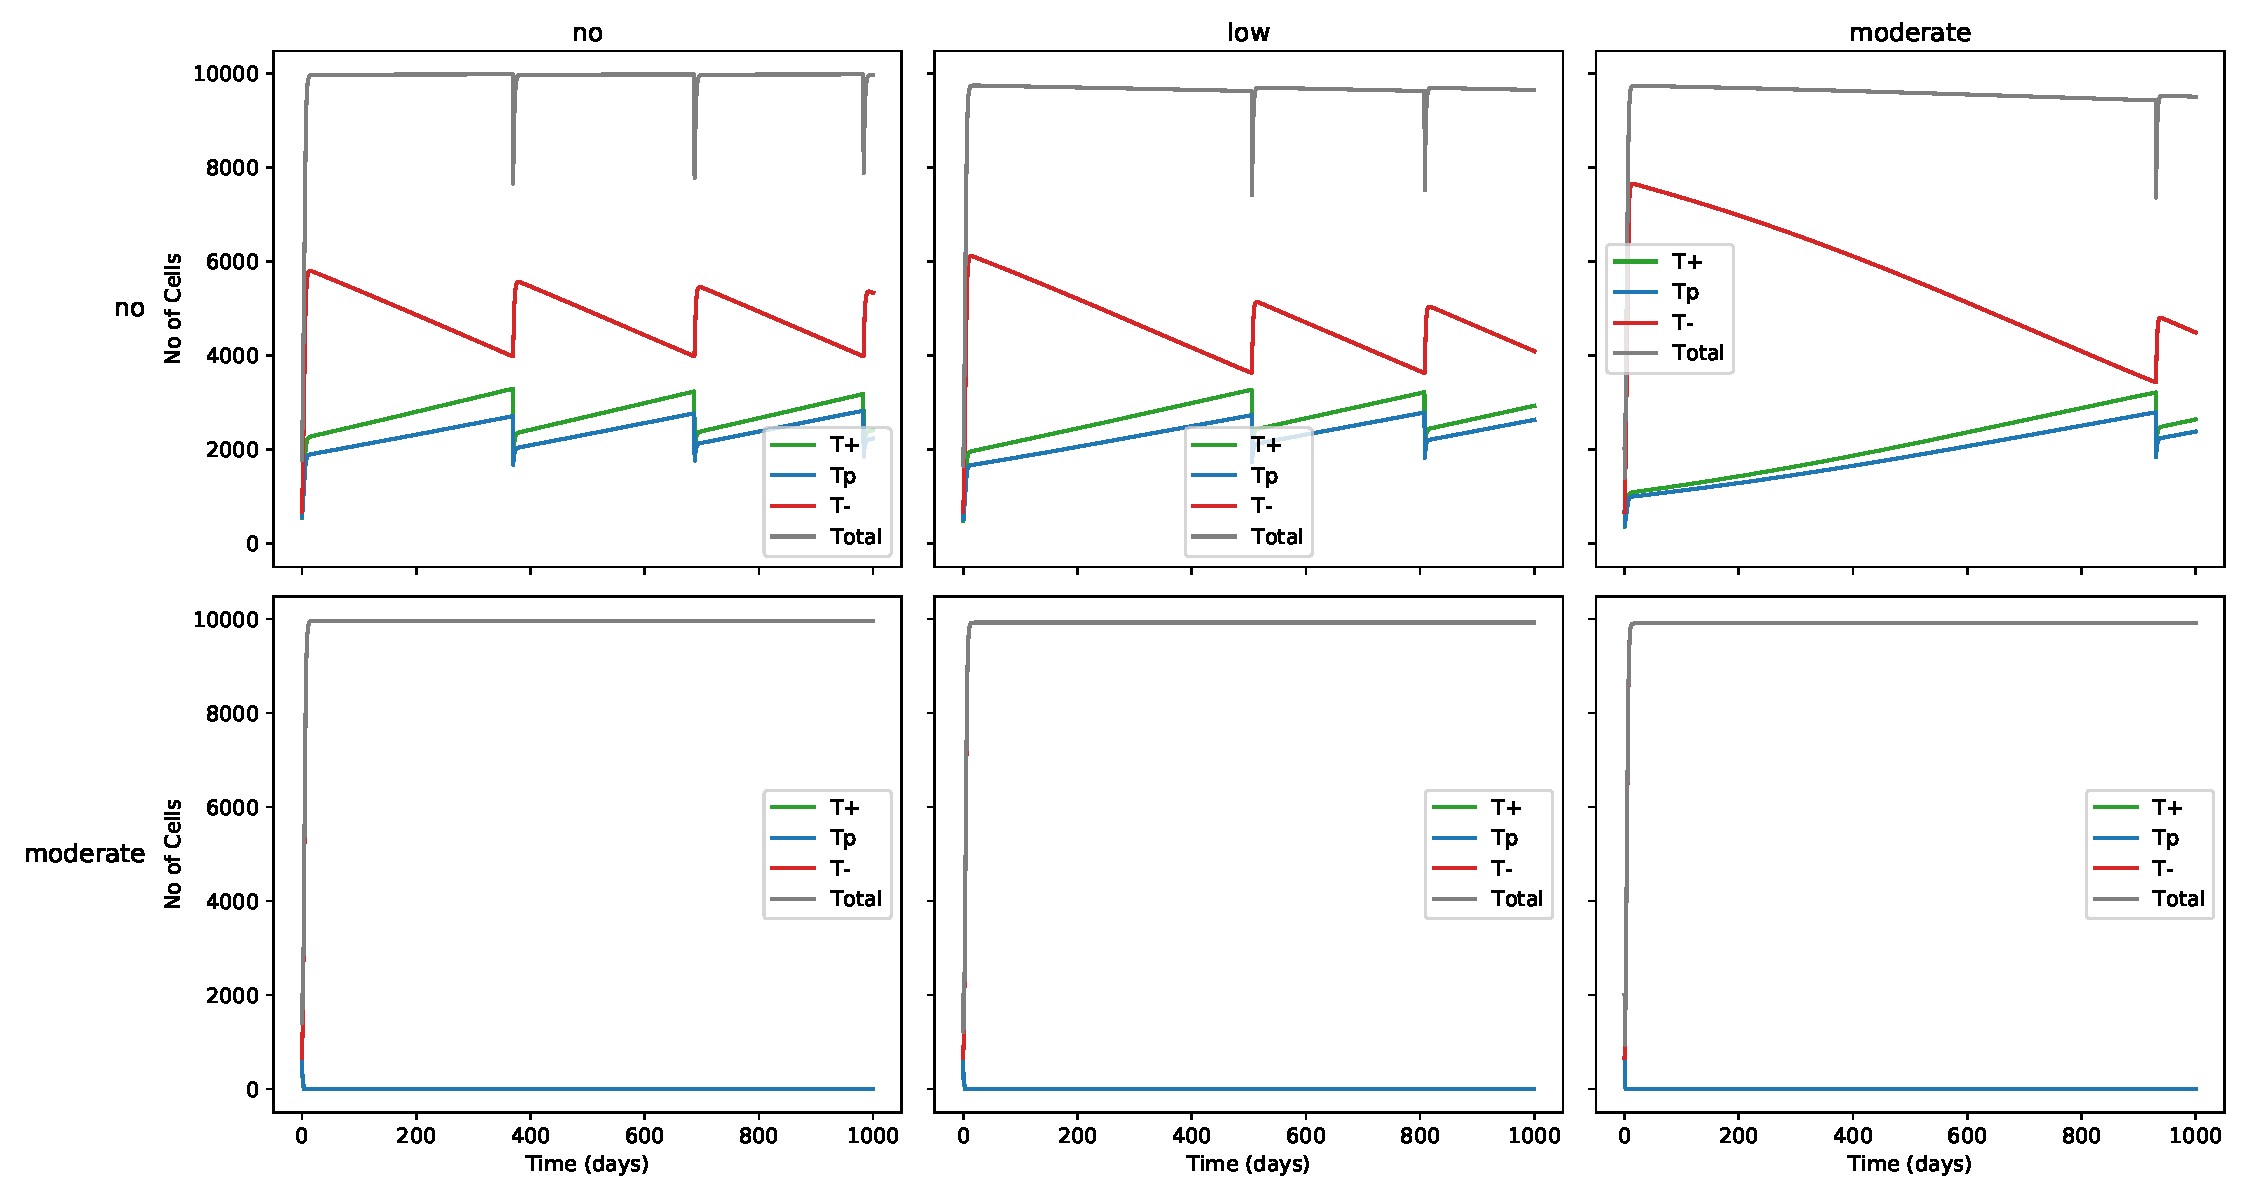
\includegraphics[width=\textwidth]{All3_therapy_200day_1:1:1}
    \caption{Equal Seeding - $T^p:T^+:T^-$ :: 1:1:1, Initial Total seeding: 2000}
    \label{fig_therapy-AT-delay200_1:1:1-2000}
  \end{subfigure}
  \begin{subfigure}[b]{\textwidth}
    \centering
    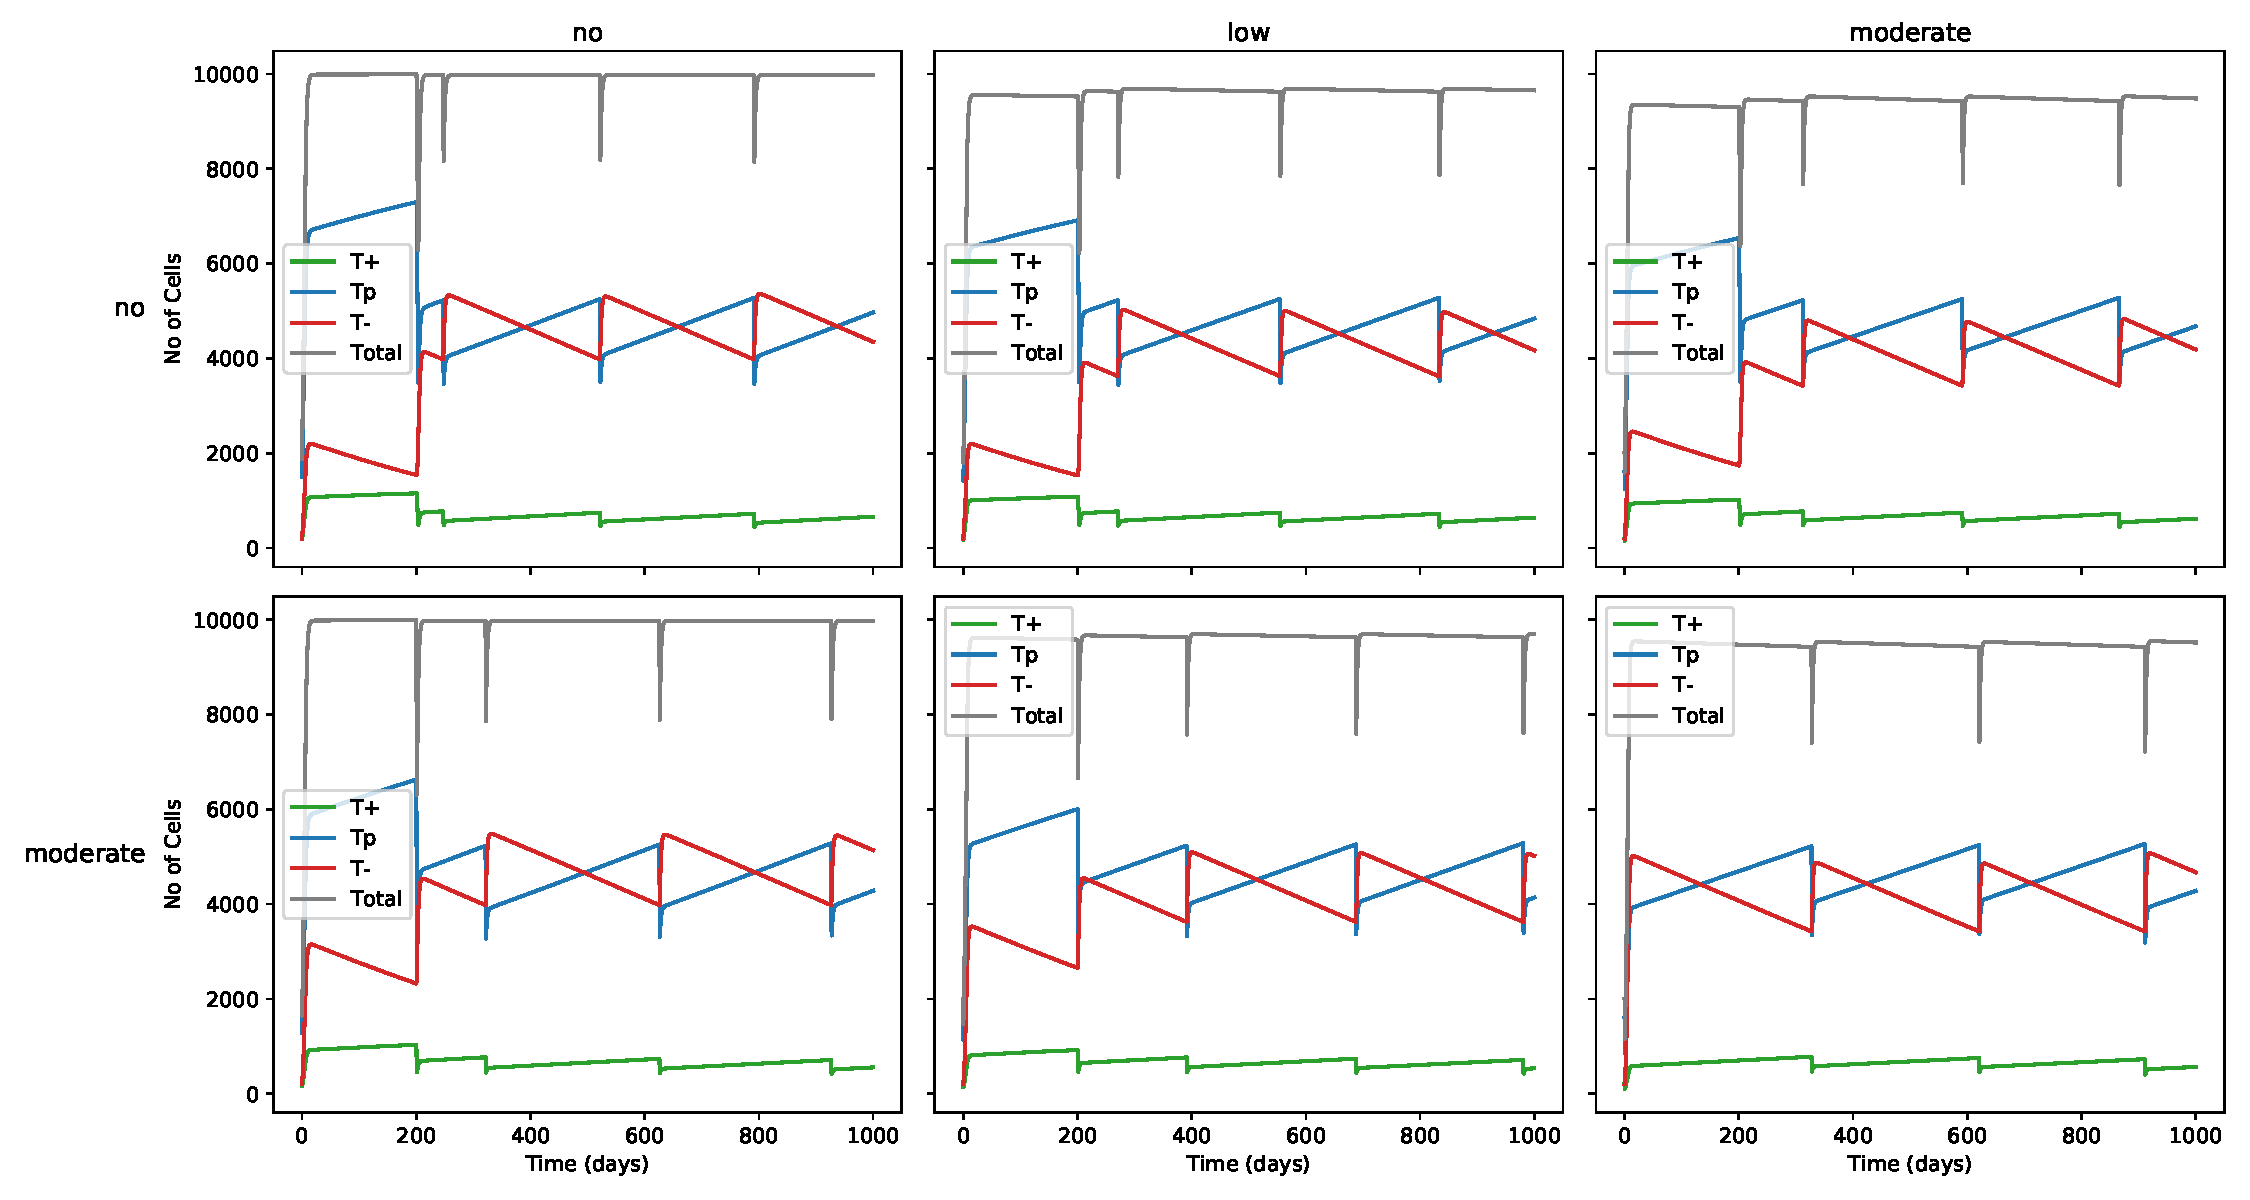
\includegraphics[width=\textwidth]{All3_therapy_200day_8:1:1}
    \caption{High $T^p$ seeding- $T^p:T^+:T^-$ :: 8:1:1, Initial Total seeding: 2000}
    \label{fig_therapy-AT-delay200_8:1:1-2000}
  \end{subfigure}
  \caption[Time-series of all cell types with delayed adaptive therapy]{Time-series of all cell types with adaptive therapy (On:6000, Off:4000) delayed by 200 days under different oxygen limitation (columns), testosterone limitation (rows) and initial seeding proportions (subfigures).}
  \label{fig_therapy-AT-delay}
\end{figure}

\clearpage

\subsection{Combination therapy with docetaxel}
Another aspect of prostate cancer therapy that could be of translational value to the model is combination therapy. Typically, hormone-specific agents like abiraterone are pairs with a general cytotoxic drug like docetaxel that causes cell death independent of cell type \cite{West}. A comprehensive exploration of combination therapy regimes would be time-consuming, but a smaller scale test-of-concept analysis was attempted here, in which AT was administered with both abiraterone and docetaxel; abiraterone was still responsive to $T^p - T^+$ alone, but docetaxel was administered based on thresholds of total population size.

Earlier data from AT with abiraterone alone leads to the expectation that there are potential spaces where docetaxel could be used to alleviate some of the $T^-$ pressure on $T^p$ and $T^+$, especially where they’re driven to extinction. However, initial data visualised in \autoref{fig_therapy-AT-combi} show that the direct negative effect of docetaxel on $T^p$ and $T^+$ outweigh any positive effect from reduction of $T^-$ competition, suggesting that the scope for docetaxel application, at least based on the current modality, is highly limited in this system as it disrupts the sensitive balance of numbers between the three cell types. Nevertheless, more extensive testing is warranted.

\begin{figure}[h!]
  \centering
  \begin{subfigure}[b]{\textwidth}
    \centering
    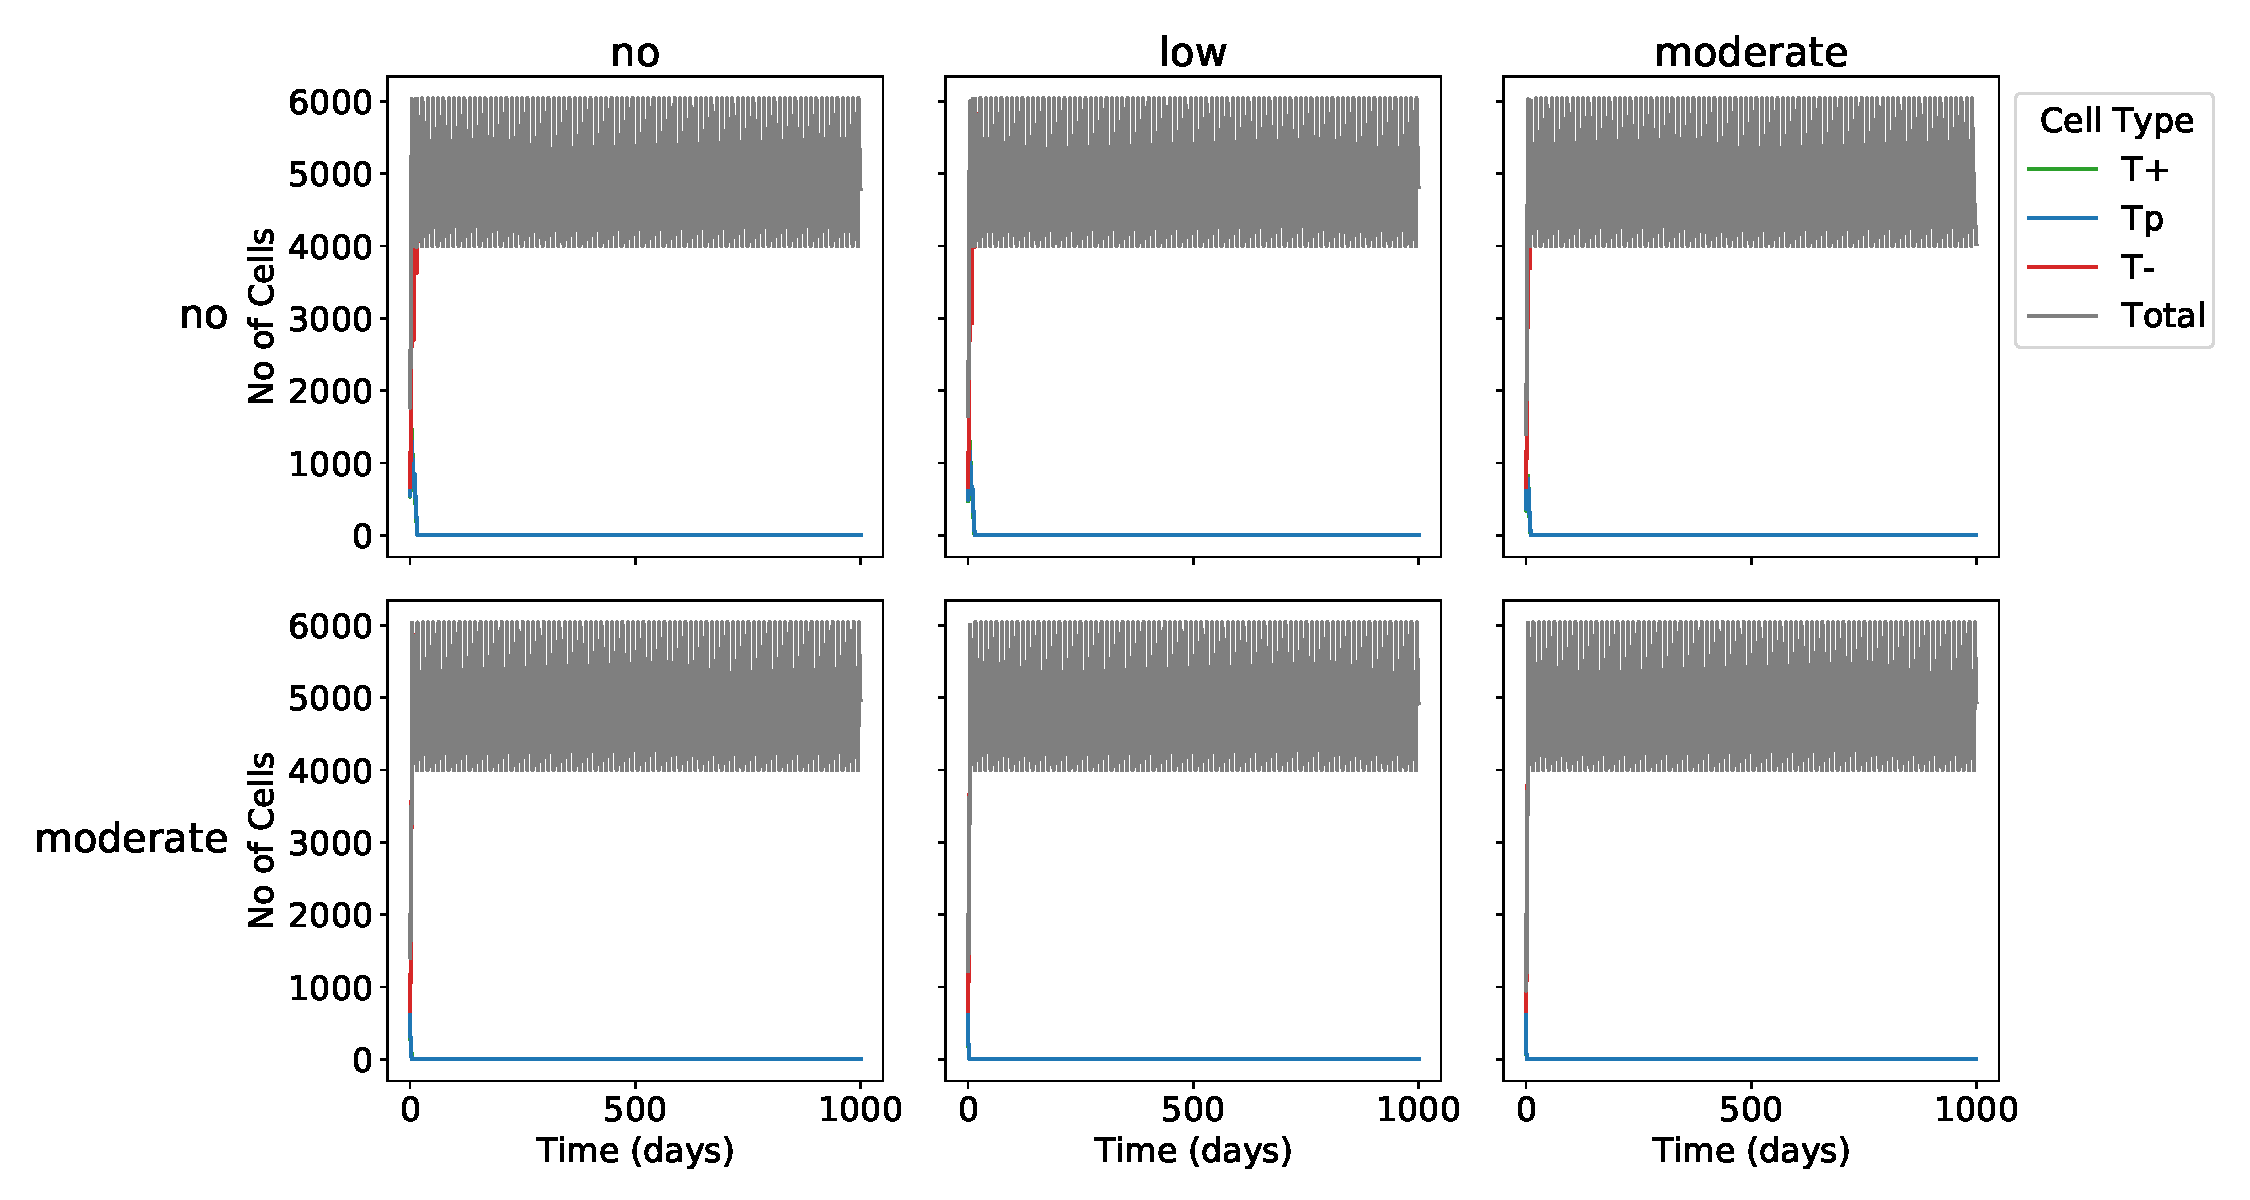
\includegraphics[width=0.9\textwidth]{All3_therapy-combi_1:1:1}
    \caption{Equal Seeding - $T^p:T^+:T^-$ :: 1:1:1, Initial Total seeding: 2000}
    \label{fig_therapy-AT-combi_1:1:1-2000}
  \end{subfigure}
  \begin{subfigure}[b]{\textwidth}
    \centering
    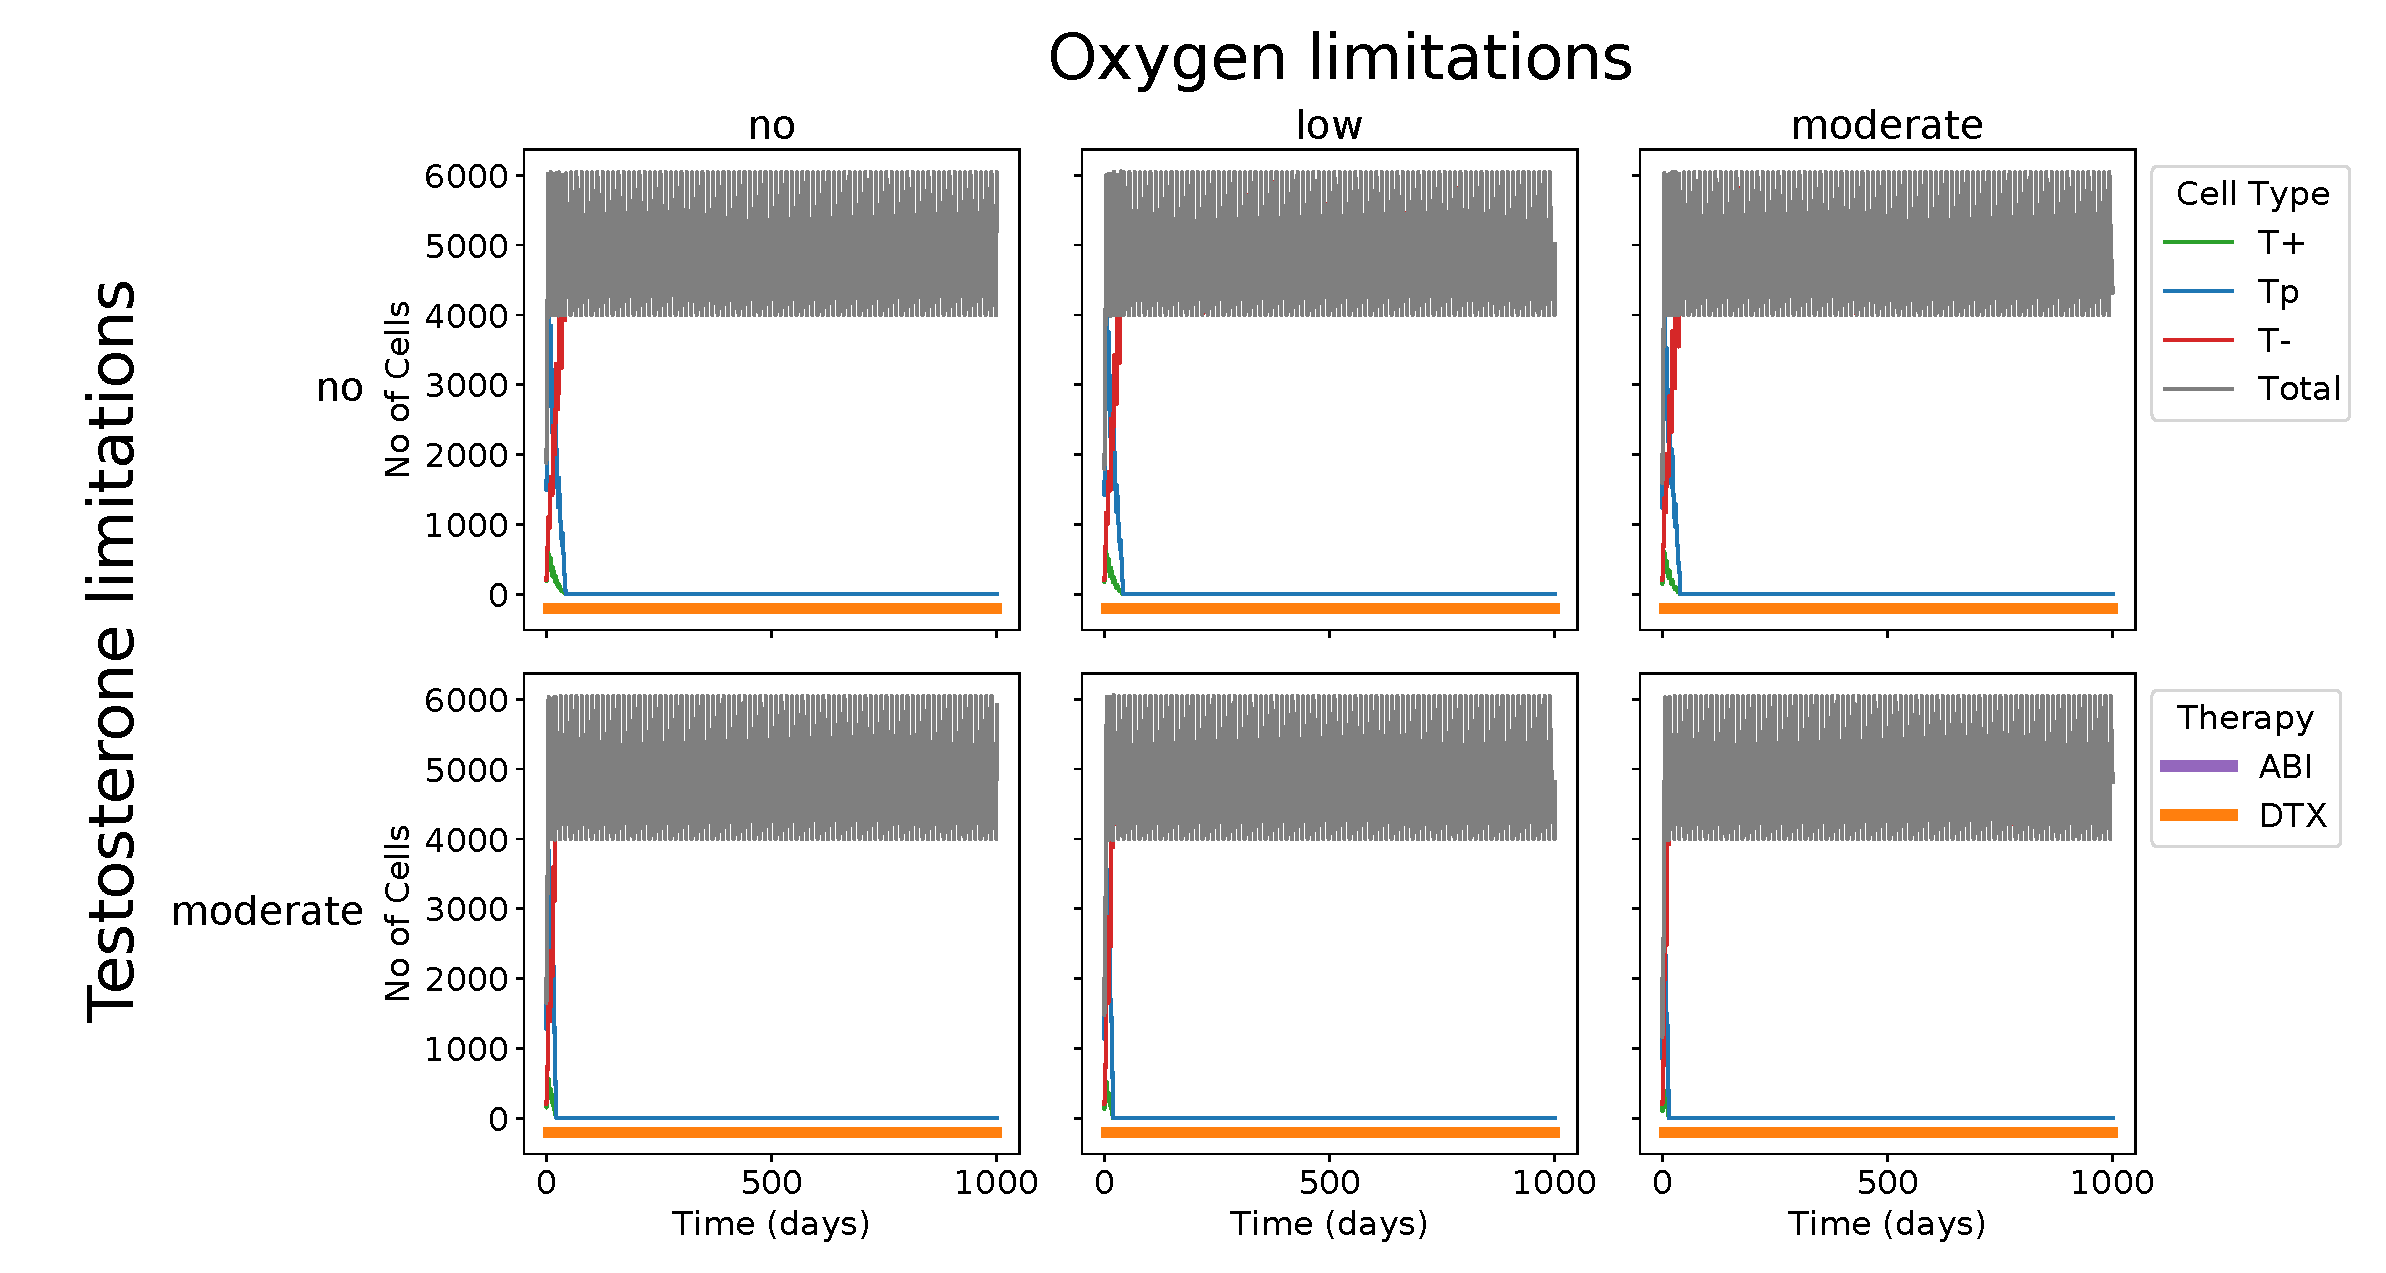
\includegraphics[width=0.9\textwidth]{All3_therapy-combi_8:1:1}
    \caption{High $T^p$ seeding- $T^p:T^+:T^-$ :: 8:1:1, Initial Total seeding: 2000}
    \label{fig_therapy-AT_combi_8:1:1-2000}
  \end{subfigure}
  \caption[Time-series of all cell types with combination adaptive therapy]{Time-series of all cell types with combination adaptive therapy of abiraterone (On:6000, Off:4000; $T^+ + T^p$) and docetaxel (On:6000, Off:4000; $T^+ + T^p + T^-$) under different oxygen limitation (columns), testosterone limitation (rows) and initial seeding proportions (subfigures). Note: The timescale of drug holiday is too small to be visible in this resolution and hence, the dtx dosage appears as a continuum.}
  \label{fig_therapy-AT-combi}
\end{figure}
